\documentclass[french]{article}
\usepackage[utf8x]{inputenc}
\usepackage[T1]{fontenc}
\usepackage{babel}
\usepackage{lmodern}
\usepackage[top=2cm,bottom=2cm,left=3cm,right=3cm]{geometry}
\usepackage{microtype}
\usepackage{mathtools, amssymb, amsthm}
\usepackage{dsfont}
\usepackage{mdframed}
\usepackage{hyperref}
\usepackage{graphicx}
\usepackage{xcolor}
\usepackage{mathrsfs}
\usepackage{wrapfig}
\usepackage{stmaryrd}
\usepackage{framed}
\usepackage{marginnote}
\usepackage{float}
\usepackage[Glenn]{fncychap}

\newtheorem{prototheorem}{Théorème}[section]
\newenvironment{thm}
   {\colorlet{shadecolor}{orange!10}\begin{shaded}\begin{prototheorem}}
   {\end{prototheorem}\end{shaded}}

\newtheorem*{protocorollary}{Corollaire}
\newenvironment{corollary}
    {\colorlet{shadecolor}{violet!10}\begin{shaded}\begin{protocorollary}}
    {\end{protocorollary}\end{shaded}}

\newtheorem*{protolemma}{Lemme}
\newenvironment{lemma}
    {\colorlet{shadecolor}{pink!15}\begin{shaded}\begin{protolemma}}
    {\end{protolemma}\end{shaded}}

\theoremstyle{definition}
\newtheorem{protodefinition}{Définition}[section]
\newenvironment{definition}
    {\colorlet{shadecolor}{green!5}\begin{shaded}\begin{protodefinition}}
    {\end{protodefinition}\end{shaded}}

\newtheorem{protoproposition}{Proposition}[section]
\newenvironment{prop}
    {\colorlet{shadecolor}{blue!5}\begin{shaded}\begin{protoproposition}}
    {\end{protoproposition}\end{shaded}}

\theoremstyle{remark}
\newtheorem*{remark}{Remarque}
\newtheorem{exo}{Exercice}
\newtheorem*{protoexemple}{Exemple}
\newenvironment{exemple}
    {\colorlet{shadecolor}{gray!10}\begin{shaded}\begin{protoexemple}}
    {\end{protoexemple}\end{shaded}}



\newcommand{\lesss}{<}
\newcommand{\less}{\lesss}

\newcommand{\biggg}{>}
\newcommand{\bg}{\biggg}

\title{\bsc{Géométrie différentielle}}
\date{2023-2024}
\author{Mohammad Reza \bsc{Pakzad}}

\begin{document}

\maketitle

\tableofcontents

\section{Fonctions continues}


$U \subseteq \mathbb{R}^n$ ouvert.

$f:
  \begin{array}{lll}
  U & \longrightarrow & \mathbb{R} \\
  (x_1, \dots, x_n) & \longmapsto f(x_1, \dots, x_n)
  \end{array}$ application.

$f$ est continue en $x_0$ dans $U$ si $$\forall \varepsilon \bg 0, \exists \delta  \bg 0, \forall x \in U, \Vert x-x_0 \Vert \less \delta \to \lvert f(x)-f(x_0) \rvert \less \varepsilon,  $$

avec $\Vert y \Vert = \sqrt{ y_1 ^2 + \dots + y_n ^2 }  $.

On dit que $f$ est une application continue quand $f$ est continue en $x \in U$ pour tout $x \in U$.

\begin{prop}
  $f$ est continue si et seulement si pour tout intervalle ouvert $J \subseteq \mathbb{R}$, $f ^{-1} (J)$ est ouvert, avec $f ^{-1} (J) := \{ x \in U \mid f(x) \in J \} $.
\end{prop}

\begin{proof}
  \begin{enumerate}
    \item \emph{Si $f$ est continue, alors $ \forall J \subset \mathbb{R}$ intervalle ouvert, $f ^{-1} (J)$ est ouvert.}

    Il faut montrer que $\forall x_0 \in f ^{-1} (J)$, il existe $r \bg 0$ tel que $B(x_0, r) \subset f ^{-1} (J)$.

    \begin{figure}[h!]
      \centering
      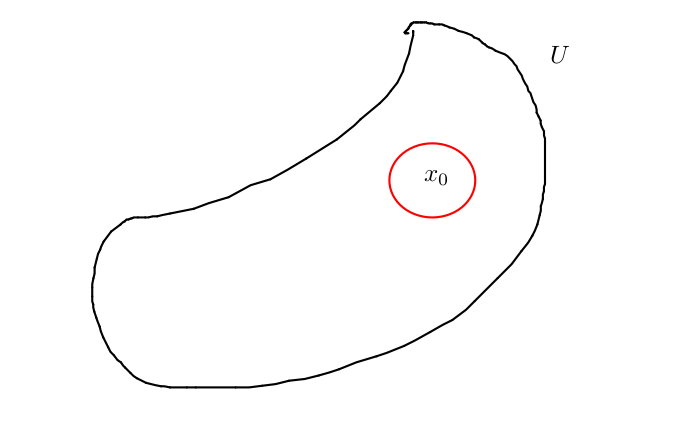
\includegraphics[scale=0.3]{figures/recip_ouvert.png}
      \caption{Illustration}
      \label{}
    \end{figure}

    $J = (a,b)$.

    $x_0 \in f ^{-1} (J) \implies f(x_0) \in J \implies a \less f(x_0) \less b \implies \exists \varepsilon  \bg 0 \text{ tel que } $

    $$ a \less f(x_0) - \varepsilon \less f(x_0) \less f(x_0) + \varepsilon \less b.$$

    On peut choisir $\varepsilon = \min \{ \frac{b-f(x_0)}{2}, \frac{f(x_0)-a}{2} \} $.

    \begin{figure}[h!]
      \centering
      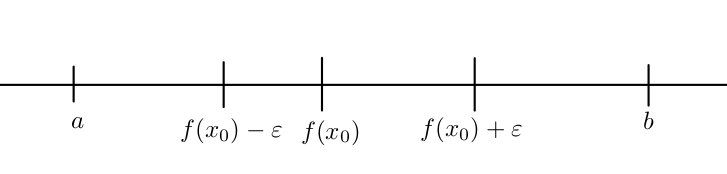
\includegraphics[scale=0.3]{figures/demo_prop_1.png}
      \caption{On choisit $\varepsilon $ de cette sorte}
      \label{}
    \end{figure}

    Donc il y a $\delta \bg 0$ tel que

    \begin{gather*}
      \Vert x-x_0 \Vert \less \delta  \implies \lvert f(x)- f(x_0) \rvert \less \varepsilon \\
      \implies - \varepsilon \less f(x) -f(x_0) \less \varepsilon \\
      \implies f(x_0) - \varepsilon \less f(x) \less f(x_0)+ \varepsilon \implies a \less f(x) \less b \\
      \implies f(x) \in J \implies x \in f ^{-1} (J).
    \end{gather*}

    Choisissons $r := \delta $

    $x \in B(x_0, r) \implies \Vert x-x_0 \Vert \less r=\delta  $.

    On a démontré que avec ce choix de $\delta $ on a $x \in f ^{-1} (J) \implies B(x_0, r) \subset f ^{-1} (J)$.

    \item \emph{Si $f ^{-1} (J)$ ouvert pour tout intervalle $J \subset \mathbb{R}$, alors $f$ est continue.}

    Fixons $x_0 \in U : \varepsilon \bg 0$ est donné.

    On met $J = (f(x_0) - \varepsilon , f(x_0)+ \varepsilon ) \neq \emptyset$.

    Par l'hypothèse, $f ^{-1} (J)$ est ouvert, donc $\exists r \bg 0, B(x_0, r) \subset f ^{-1} (J)$.

    On met $\delta := r$.

    \begin{gather*}
      \Vert x-x_0 \Vert \less \delta \implies x \in B(x_0, \delta ) = B(x_0, r)\\
      \implies x \in f ^{-1} (J) \implies f(x) \in J \\
      \implies f(x_0) - \varepsilon \less f(x) \less f(x_0) + \varepsilon \implies - \varepsilon \less f(x) - f(x_0) \less \varepsilon \\
      \implies \lvert f(x) - f(x_0) \rvert \less \varepsilon .
    \end{gather*}
  \end{enumerate}
\end{proof}

On peut aussi généraliser ces définitions et la proposition aux cas où $f: U \to \mathbb{R}^m$ est une application de $U$ dans $\mathbb{R}^m$, avec

$$ f(x_1, \dots, x_n) = (f_1(x_1, \dots, x_n), \dots, f_m(x_1, \dots, x_m)).$$

\paragraph{Exemple}

$f(x_1, x_2) = (x_1 ^2+ 3 \cos(x_2) e^{x_1-x_2} )$, $n=2, m=2, U = \mathbb{R}^2$.

\begin{definition}
  $f$ est continue en $x_0 \in U$ si

  $$ \forall \varepsilon  \bg 0, \exists \delta  \bg 0, \forall x \in U, \Vert x-x_0 \Vert \less \delta \implies \Vert f(x)-f(x_0) \Vert \less \varepsilon, $$

  avec   $\Vert f(x)-f(x_0) \Vert = \sqrt{ (f_1(x)-f_1(x_0)) ^2 + \dots + (f_m(x)-f_m(x_0)) ^2 } $.
\end{definition}

\begin{definition}
  $f : U \to \mathbb{R}^m$ est continue quand $f$ est continue en $x, \forall x \in U$.
\end{definition}

\begin{prop} \label{continue}
  Les 3 conditions suivantes sont équivalentes.

  \begin{enumerate}
    \item $f : U \to \mathbb{R}^m$ est continue ;
    \item $\forall j \in \{ 1, \dots, m \} $, $f_j$ est continue ;
    \item $\forall V \subseteq \mathbb{R}^m$ ensemble ouvert, $f  ^{-1} (V)$ est ouvert.
  \end{enumerate}
\end{prop}

\begin{figure}[h!]
  \centering
  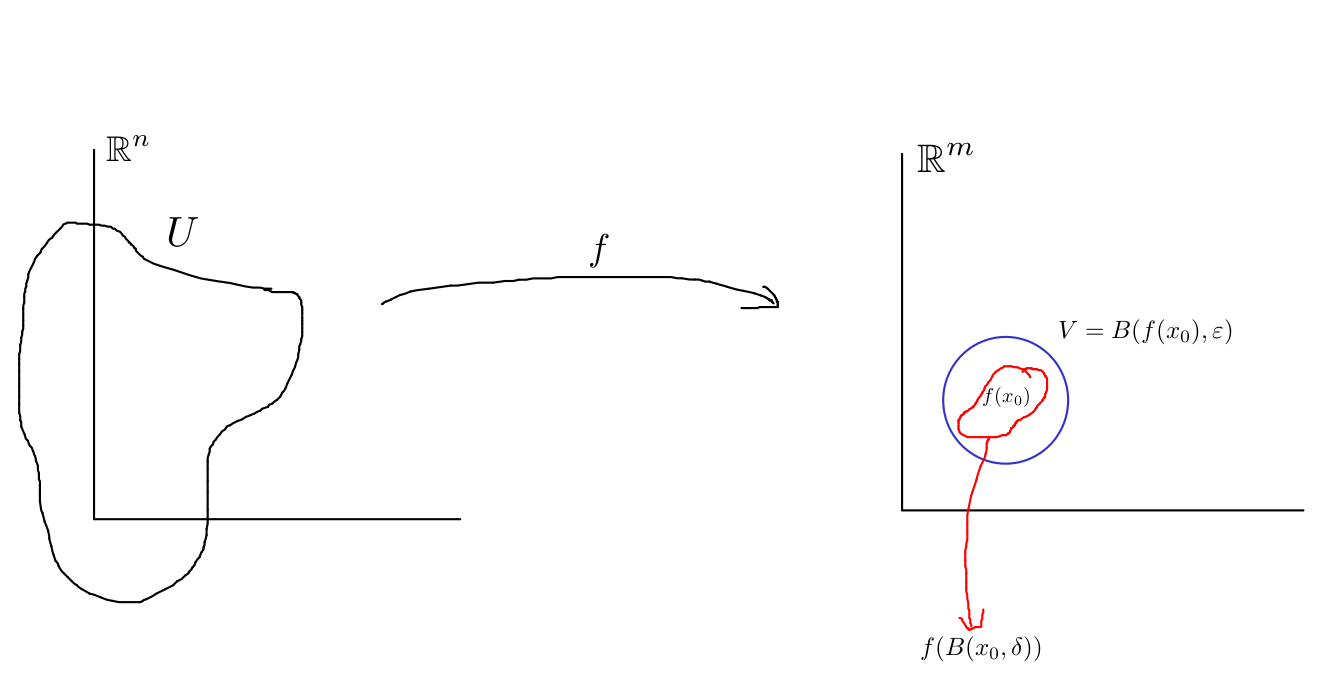
\includegraphics[scale=0.2]{figures/boule_continue.png}
  \caption{Illustration pour \ref{continue}}
  \label{}
\end{figure}



\section{Dérivée, dérivée partielle, différentielle}

$ f : U \to \mathbb{R}$.

$x \in U$ fixé.

La dérivée partielle $\frac{\partial f }{\partial x_i} $, pour $ i \in \{ 1, \dots, n \} $ et $x = (x_1, \dots, x_n)$ est définie par

\begin{gather*}
  \frac{\partial f }{\partial x_i} (x_1, \dots, x_n) := \lim_{h \to 0} \frac{f(x_1, \dots, x_i + h, \dots, x_n)}{h}
\end{gather*}

si la limite existe.

Si $e_i \in \mathbb{R}^n$ est le vecteur $e_i = (0,0,  \dots, 0, \overbrace{1}^{i\text{-ème}}, 0, \dots, 0)$ (tel que $\{ e_1, \dots, e_n \} $ est la base standart de l'espace linéaire $\mathbb{R}^n$), on a

\begin{gather*}
  \frac{\partial f }{\partial x_i }(x) := \lim_{h \to 0} \frac{f(x+h e_i)}{h}  .
\end{gather*}

On peut aussi calculer les dérivées partielles de $\frac{\partial f }{\partial x_i} $. En général, pour tout $k \geq 1$, $$ \frac{\partial ^{k} f }{\partial x_k \partial x _{k-1} \dots \partial x_2 \partial x_1 }  = \frac{\partial  }{\partial x_k } \left(\frac{\partial  }{\partial x _{k-1} } \dots \left(\frac{\partial f }{\partial x_1} \right) \right) .$$

$i_1 \in \{ 1, \dots, n \}, \dots, i_k \in \{ 1, \dots, n \} $.

Pour $k=1$, il y a $n$ dérivées partielles.

Pour $k=2, i_1 \longrightarrow$ $n$ choix de $\{ 1, \dots, n \} $.

$i_2 \longrightarrow $ $n$ choix.

Donc il y a $n ^2$ choix.

En général, il y a $n ^{k}$ dérivées partielles différentes de l'ordre $k$.

\begin{definition}
  $r \in \mathbb{N}$.

  On dit que $f : U \to \mathbb{R}$ est une application de classe $\mathcal{C}^r$  ou tout simplement $f$ est $\mathcal{C}^r$ quand

  \begin{enumerate}
    \item Si $r=0$, $f$ est continue.
    \item Si $r \geq 1$, $f$ est continue et les dérivées partielles d'ordre $k$ existent partout dans $U$ et elles sont toutes les applications continues dans $U$ et ceci pour tout $ 1 \leq k \leq r$.
    \item Pour $f : U \to \mathbb{R}^m$, une application, on dit que $f$ est $\mathcal{C}^r$ si $\forall j \in \{ 1, \dots, m \} $, $f_j$ est une application $\mathcal{C}^r$, avec $f = (f_1, \dots, f_m)$.

    On dit que $f$ est $\mathcal{C}^\infty$ quand $\forall r \in \mathbb{N}$, $f$ est $\mathcal{C}^r$.
  \end{enumerate}
\end{definition}

\subsection{Différentiabilité des fonctions multi-variables}

$U \subseteq \mathbb{R}^n$ ouvert, $f : U \to \mathbb{R}^n$, $x=(x_1, \dots, x_n) \in U$, $f = (f_1, \dots, f_m)$.

On dit que $f$ est différentiable à $x \in U$ quand il existe une application linéaire $L : \mathbb{R}^n \to \mathbb{R}^m$ telle que

\begin{gather*}
  \forall \varepsilon \bg 0, \exists \delta  \bg 0 \text{ si } \Vert h \Vert \less \delta \text{ et } x+h \in U, \text{ alors } \Vert f(x+h) - (f(x)+L(h)) \Vert \less \varepsilon \Vert h \Vert .
\end{gather*}

\begin{figure}[h!]
  \centering
  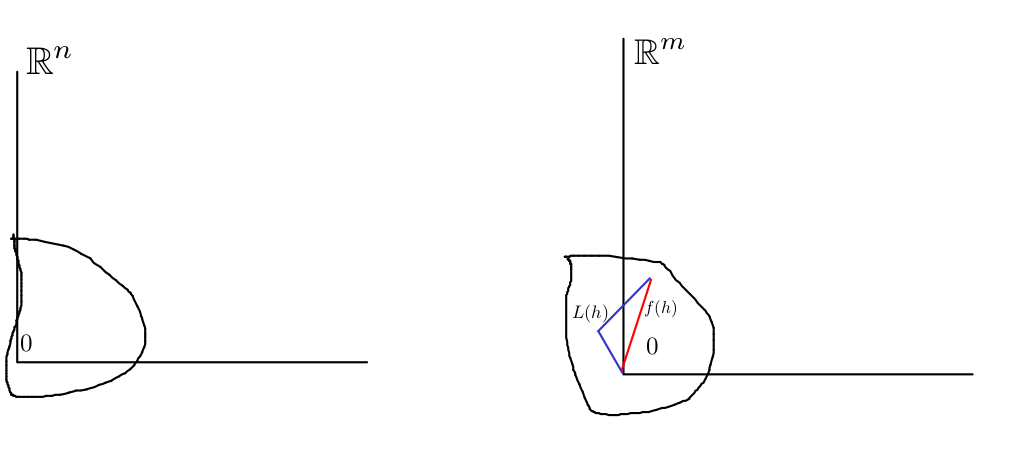
\includegraphics[scale=0.3]{figures/diff.png}
  \caption{Exemple illustratif avec $x=0, f(0) = 0$}
  \label{}
\end{figure}

$f$ différentiable en 0 si $\forall \varepsilon  \bg 0$, $\exists \delta \bg 0, \Vert h \Vert \less \delta \implies \Vert f(h) - L(h) \Vert \less \varepsilon \Vert h \Vert  $.

\begin{prop}
  $n=1, m=1, f : I \to \mathbb{R}$ est différentiable selon la définition donnée sur un point $x \in I$ si et seulement si $f'(x)$ existe.
\end{prop}

\begin{proof}

  \

  \begin{enumerate}
    \item \emph{Sens direct : $f$ différentiable en $x \in I$ $\implies f'(x)$ existe.}

    $\exists L : \mathbb{R} \to \mathbb{R}$ telle que

    $$ \forall \varepsilon \bg 0, \exists \delta \bg 0, \Vert h \Vert \less \delta , x+h \in I \implies \Vert f(x+h) - f(x) -L(h) \Vert \less \varepsilon \Vert h \Vert.$$

    $L(h) = ah$ pour un $a \in \mathbb{R}$ quelconque mais fixé.

    $a$ est la pente ou le coefficient directeur.

    Prenons $a$   la pente du graphe de $L$ (comme $L$ linéaire, $\exists a \in \mathbb{R}$ tel que $\forall h \in \mathbb{R}, L(h) = ah$).

    On obtient

    $$ \forall \varepsilon \bg 0, \exists \delta \bg 0, \lvert h \rvert \less \delta , x+h \in I \implies \lvert f(x+h) -f(x)-ah \rvert \leq \varepsilon \lvert h \rvert.$$

    On divise par $\lvert h \rvert \neq 0$ pour obtenir

    \begin{gather*}
      \left\lvert \frac{f(x+h)-f(x)}{h} - \frac{ah}{h} \right\rvert \leq \varepsilon.
    \end{gather*}

    \begin{gather*}
      \forall \varepsilon  \bg 0, \exists \delta  \bg 0 \text{ tel que } \lvert h \rvert \less \delta , h+x \in I, \text{ alors } \left\lvert \frac{f(x+h)-f(x)}{h}-a \right\rvert \leq \varepsilon,
    \end{gather*}

    c'est à dire

    \begin{gather*}
      \lim_{h \to 0} \frac{f(x+h)-f(x)}{h} = a.
    \end{gather*}

    Donc $f'(x)$ existe et $f'(x) = a$.

    \item \emph{Sens réciproque : $f'(x)$ existe $\implies f$ différentiable.}

    Si $f'(x)$ existe, on met $a :=f'(x)$.

    On définit $L(h) =ah$. On sait que

    $$ \lim_{h \to 0} \frac{f(x+h)-f(x)}{h} = f'(x) = a.$$

    Donc

    \begin{gather*}
      \forall \varepsilon \bg 0, \exists \delta  \bg 0, \lvert h \rvert \less \delta \implies \left\lvert \frac{f(x+h)-f(x)}{h} -a \right\rvert \leq \varepsilon  \\
      \implies \lvert f(x+h) -f(x) -ah \rvert \leq \varepsilon \lvert h \rvert \\
      \implies \forall h, \lvert h \rvert \less \delta, \text{ on a } \lvert f(x+h) - f(x) -ah \rvert \leq \varepsilon \lvert h \rvert.
    \end{gather*}

    $f$ est différentiable selon notre définition avec $L(h) =ah$.
  \end{enumerate}
\end{proof}


On suppose maintenant que $f:U \to \mathbb{R}^m, U \subseteq \mathbb{R}^n$.

Pour $x \in U$, $f$ différentiable en $x$ si $\exists L : \mathbb{R}^n \to \mathbb{R}^m$ linéaire telle que

\begin{gather*}
  \forall \varepsilon  \bg 0, \exists \delta  \bg 0, \forall h \in \mathbb{R}^n, \Vert h \Vert \less \delta, x+h \in U \implies \Vert f(x+h) -f(x)-L(h) \Vert \leq \varepsilon \Vert h \Vert.
\end{gather*}

On note $\mathscr{L}(\mathbb{R}^n, \mathbb{R}^m) = \{  T: \mathbb{R}^n \to \mathbb{R}^m \mid T \text{ est linéaire }   \} $.

On écrit dans ce cas là que $Df(x) = L \in \mathscr{L}(\mathbb{R}^n, \mathbb{R}^m)  $.

En particulier, si $f$ est différentiable pour tout $x \in U$, on obtient une application $$Df : U \to \mathscr{L}(\mathbb{R}^n, \mathbb{R}^m). $$

\subparagraph{Rappel} Chaque transformation linéaire est uniquement représentée par une matrice au cas où les bases des espaces de départ et d'arrivée sont fixées.

Si on choisit les bases standart $\alpha = \{ e_1, \dots, e_n \} $ pour $ \mathbb{R}^n$ et $ \beta = \{ e_1, \dots, e_m \} \in \mathbb{R}^m $, $T \in \mathscr{L}(\mathbb{R}^n, \mathbb{R}^m) $.

$$ [T] _{\beta } ^{\alpha} := A = [A _{ij}] _{m \times n}$$

et on a $$ T(e_j) = \sum_{i=1}^{m} A _{ij} e_i  = \begin{pmatrix}
  A _{1j} \\
  A _{2j} \\
  \vdots \\
  A _{mj}
\end{pmatrix}.$$

C'est la j-ième colonne de la matrice $A$.

En particulier, pour chaque $x \in U$ où $f$ est différentiable, en fixant les bases standart de $\mathbb{R}^n$ et $\mathbb{R}^m$, on peut supposer que $Df(x) \in \mathbb{R} ^{m \times n}$.

On peut identifier $\mathscr{L}(\mathbb{R}^n, \mathbb{R}^m) $ avec $\mathbb{R} ^{m \times n} = \{ [A _{ij}], 1 \leq i \leq n, 1 \leq j \leq m \mid A _{ij} \in \mathbb{R}\} $.

Avec cette identification, on peut utiliser la norme euclidienne de $\mathbb{R} ^{m \times n}, \Vert A \Vert = \left( \sum_{i=1}^{n} \sum_{j=1}^{m} \lvert A _{ij} \rvert ^2 \right) ^{\frac{1}{2}}  $.

Comme ça on peut parler de continuité et de différentiabilité de l'application $$Df : U \to \mathscr{L}(\mathbb{R}^n, \mathbb{R}^m) \simeq \mathbb{R}^{m\times n}.$$

Ou bien on peut encore identifier $\mathbb{R} ^{m \times n}$ avec $\mathbb{R} ^{mn}$. Alors $Df : U \subseteq \mathbb{R}^n \to \mathbb{R} ^{mn}$.

Donc on peut parler de continuité de $Df $, de derivée de $Df$.

Pour $x \in U, D(Df)(x) \in \mathscr{L}(\mathbb{R}^n, \mathscr{L}(\mathbb{R}^n, \mathbb{R}^m) ) $.

On va noter $D(Df)$ par $D ^2f$. Alors $D ^2 f (x) \in \mathscr{L}(\mathbb{R}^n, \mathscr{L}(\mathbb{R}^n, \mathbb{R}^m) ) = \mathscr{L}(\mathbb{R}^n, \mathbb{R}^{m\times n})  $.

$D ^2 f : U \to \mathscr{L}(\mathbb{R}^n, \mathbb{R} ^{m \times n}) \simeq \mathbb{R} ^{mn ^2} $.

\begin{thm}
  $f : U \to \mathbb{R}^m$ une application donnée et $r \in \mathbb{N}$.

  $f$ est de classe $\mathcal{C}^r$ si et seulement si $D ^{k} f : U \to \mathscr{L}(\mathbb{R}^n, \mathscr{L}(\mathbb{R}^n, \dots) ) \ (\text{de dimension } mn ^{k}) $ existe comme une application pour tout $1 \leq  k \leq r$, et elle est en plus continue.
\end{thm}

\subsection{Deux points fins}

En général, les dérivées partielles de $f$ peuvent exister sans que $Df$ soit définie.

Par exemple, dans $\mathbb{R}^2$, on peut avoir $f$ telle que $\frac{\partial f }{\partial x_1 }(0) $ existe, $\frac{\partial f }{\partial x_2 } $ existe, mais $Df(0)$ n'existe pas.

Par contre, si $Df(x_0)$ existe, alors toutes les dérivées partielles de $f$ existent en $x_0$.

\begin{proof}
  Supposons que $Df(x_0)$ existe. Donc

  $$ \forall \varepsilon \bg 0, \exists \delta \bg 0, \Vert h \Vert \less \delta , x+h \in U  \implies \Vert f(x) -f(x_0) - L(h) \Vert \less \varepsilon \Vert h \Vert . $$

  Fixons une direction $\overrightarrow{ v } \in \mathbb{R}^n$ et on met $h = t \overrightarrow{ v } $, avec $\Vert \overrightarrow{ v }  \Vert \neq 0$. Donc $\Vert h \Vert = \lvert t \rvert \cdot \Vert \overrightarrow{ v }  \Vert  $.

  Donc

  \begin{gather*}
    \forall \varepsilon \bg 0, \exists \delta  \bg 0, t \less \frac{\delta }{\Vert \overrightarrow{ v }  \Vert}, x_0 + t \overrightarrow{ v }  \in U \implies \lvert f(x_0+t \overrightarrow{ v } )-f(x_0)-tL(\overrightarrow{ v } ) \rvert \less \varepsilon \lvert t \rvert \Vert \overrightarrow{ v }  \Vert .
  \end{gather*}

  On pose $\tilde{\varepsilon } = \varepsilon  \Vert \overrightarrow{ v }  \Vert \text{ et }  \tilde{\delta } = \frac{\delta }{\Vert \overrightarrow{ v }  \Vert } $.

  \begin{gather*}
    \forall \tilde{\varepsilon } \bg 0, \exists \tilde{ \delta } \bg 0 \text{ tel que } \lvert t \rvert \less \tilde{\delta } \implies \Vert f(x_0+t \overrightarrow{ v } ) -f(x_0)-tL(\overrightarrow{ v } ) \Vert   \leq \tilde{\varepsilon } \\
    \forall \tilde{\varepsilon } \bg 0, \exists \tilde{ \delta } \bg 0, \lvert t \rvert \less \tilde{\delta } \implies \left\Vert \frac{1}{t}\left(f(x_0 + t \overrightarrow{ v } ) -f(x_0)) - L(\overrightarrow{ v } \right) \right\Vert \leq \tilde{\varepsilon } \\
    \implies \lim_{t \to 0} \frac{1}{t}\left(f(x_0+t \overrightarrow{ v } )-f(x_0)\right) = L(\overrightarrow{ v } ) = Df(x_0)(\overrightarrow{ v } ) .
  \end{gather*}

  On définit
  \begin{equation*}
    D _{\overrightarrow{ v } }f(x_0) := \lim_{t \to 0} \frac{1}{t}(f(x_0+t \overrightarrow{ v } )-f(x_0)).
  \end{equation*}

  Donc si $Df(x_0)$ existe, la dérivée directionnelle de $f$ en $x_0$ dans une direction $\overrightarrow{ v } \in \mathbb{R}^n$ existe et on a

  $$ D \overrightarrow{ v } f(x_0) = Df(x_0)(\overrightarrow{ v } ) \in \mathbb{R}^m.$$

  En particulier, si $\overrightarrow{ v } = e_j, 1 \leq j \leq n $,
  \begin{equation*}
    \frac{\partial f }{\partial x_j }f(x_0) = D _{e _{j}} f(x_0) = Df(x_0)(e_j).
  \end{equation*}
\end{proof}

Il se peut que toutes les dérivées directionnelles $D _{\overrightarrow{ v } }f(x_0)$ existent pour tout $\overrightarrow{ v } \in \mathbb{R}^n $ alors que $Df(x_0)$ n'existe pas.

\

\begin{thm}
  Si $f : U \to \mathbb{R}^m, x_0 \in U$.

  Si $Df(x_0)$ existe, alors $f$ est continue en $x_0$.
\end{thm}

\begin{proof}
  En exercice.
\end{proof}

Il se peut que toutes les dérivées directionnelles $D _{\overrightarrow{ v } } f(x_0)$ existent pour tout $\overrightarrow{ v } \in \mathbb{R}^n$ en $x_0 \in U$ sans que pour autant $f$ soit continue en $x_0$.

Si la matrice de $Df(x_0)$ est donnée par $[A _{ij}] _{\substack{1 \leq i \leq n \\ 1 \leq j \leq m}}$.

$$ \forall j \in \{ 1, \dots, n \}, A _{e_j} = \frac{\partial f }{\partial x_j}(x_0) = \left[ \begin{matrix}
  \frac{\partial f_1 }{\partial x_j}(x_0) \\
  \vdots \\
  \frac{\partial f_m }{\partial x_j}(x_0)
\end{matrix} \right].$$

$$ Df = \left[ \begin{matrix}
  \frac{\partial f_1 }{\partial x_1 } & \dots & \frac{\partial f_1 }{\partial x_n }  \\
  \vdots & \ddots & \vdots \\
  \frac{\partial f_m }{\partial x_1 } & \dots & \frac{\partial f_m}{\partial x_n }
\end{matrix} \right].$$

C'est la matrice jacobienne de $f$.

\

\subsection{La dérivée de composition}

$f : \mathbb{R} \to \mathbb{R}$, $g : \mathbb{R} \to \mathbb{R}$, $(g \circ f)'(x) = g'(f(x))f'(x)$.

$f : U \to \mathbb{R}^m$, $g : V \to \mathbb{R}^p$.

Supposons que pour $x_0 \in U$, $f(x_0) \in V$.

\begin{figure}[h!]
  \centering
  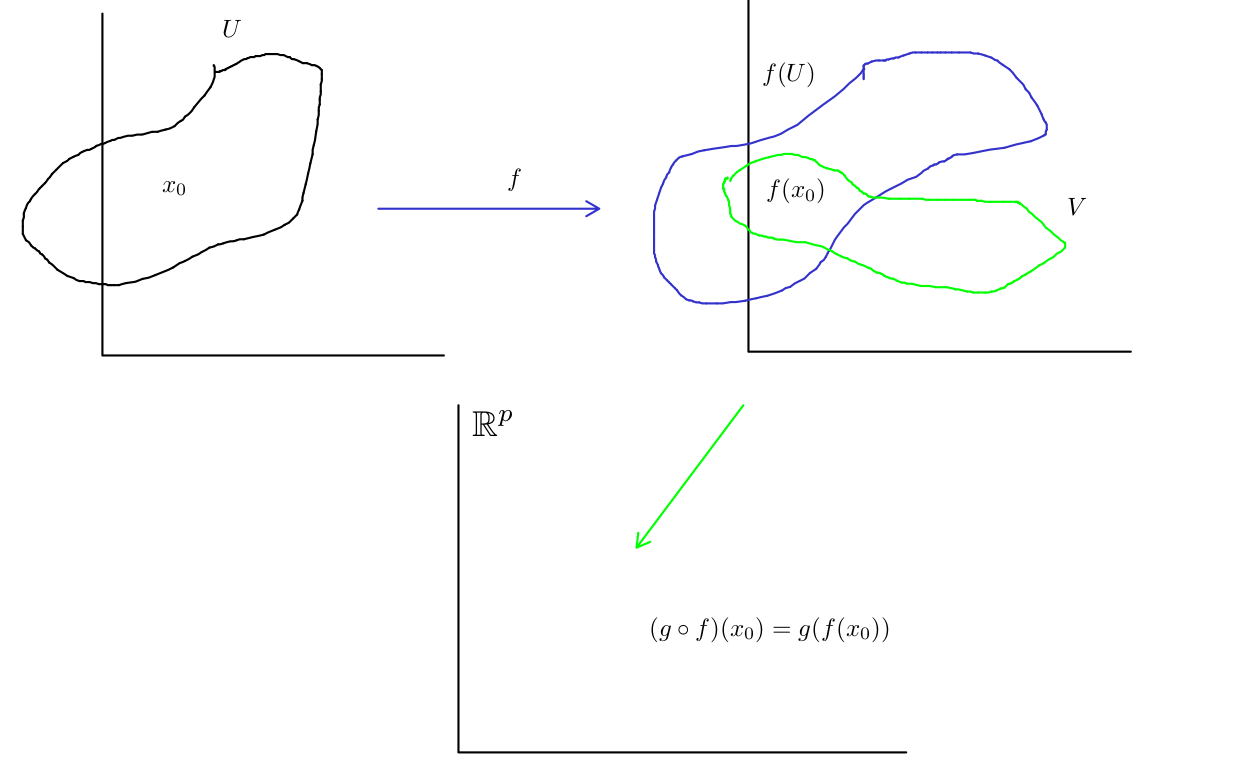
\includegraphics[scale=0.3]{figures/composition.png}
  \caption{La différentiation composée}
  \label{}
\end{figure}

Si $f$ est continue, $g \circ f$ est définie dans un voisinage de $x_0$, par exemple dans une boule ouverte $B(x_0, r) = \tilde{U} \subset U \cap f ^{-1} (V)$.

$g \circ f : \tilde{U} \to \mathbb{R}^p$.

Supposons que les trois dérivées $Df(x_0), Dg(f(x_0)), D(g \circ f)(x_0)$ existent.

$Df(x_0) \in \mathscr{L}(\mathbb{R}^n, \mathbb{R}^m) $.

$D(g(f(x_0))) \in \mathscr{L}(\mathbb{R}^m, \mathbb{R}^p) $.

$D(g \circ f) \in (\mathbb{R}^n, \mathbb{R}^p)$.

\begin{thm}
  Supposons que $f$ est dérivable en $x_0 \in U$ avec la dérivée $Df(x_0)$ et $g$ est dérivable en $f(x_0) \in V$ avec la dérivée $Dg(f(x_0))$, alors $g \circ f$ est bien dérivable en $x_0 \in U$ et

  $$ D(g \circ f)(x_0) = Dg(f(x_0)) \circ Df(x_0).$$
\end{thm}

Si on utilise les matrices jacobiennes de chaque dérivée ($1 \leq k \leq m, 1 \leq j \leq n, 1 \leq i \leq p$),

\begin{gather*}
  \left[ \frac{\partial (g \circ f)_i }{\partial x_j}  \right]_{p \times n}(x_0) = \left[ \frac{\partial g_i }{\partial y_k }  \right] _{p \times m}(f(x_0))  \times \left[ \frac{\partial f_k }{\partial x_j} \right] _{m \times n}(x_0).
\end{gather*}

\begin{gather*}
  \left[ \frac{\partial z_i }{\partial x_j } \right](x_0) = \left[ \frac{\partial z_i }{\partial y_k } \right](f(x_0)) \times \left[\frac{\partial y_k }{\partial x_j} \right](x_0).
\end{gather*}

On a :

$$ \frac{\partial z_i }{\partial x_j } (x_0) = \sum_{k=1}^{n} \frac{\partial z_i }{\partial y_k}  (f(x_0)) \frac{\partial y_k }{\partial x_j} (x_0). $$

$f : U \to \mathbb{R}^m, U \subseteq \mathbb{R}^n$, $V = f(U)$ est ouvert et $g : V \to \mathbb{R}^n$ est l'inverse de $f$.

Donc $g \circ f : U \to \mathbb{R}^n$ et $g \circ f = \mathds{1} _{U}$.

Si en plus $f$ et $g$ sont différentiables, alors $m=n$ et $\forall x \in U, Dg(f(x)) = (Df(x)) ^{-1} $, c'est à dire en particulier $Df(x)$ est une transformation linéaire inversible.

\begin{proof}
  Si $f$ est dérivable en $x \in U$ et $g$ dérivable en $f(x) \in V$,  $\mathds{1} = g \circ f$ dérivable en $x_0$ et

  $$ D \mathds{1} _{U}(x_0) = D(g(f(x_0))) \circ Df(x_0).$$

  $$ \mathds{1} _{U}(x) = x \implies D \mathds{1} _{U}(x_0) \in \mathscr{L}(\mathbb{R}^n, \mathbb{R}^n).$$

  Donc  $$ \mathds{1} _{\mathbb{R}^n} = Dg(f(x_0)) \circ Df(x_0).$$

  Ainsi comme $g$ est linéaire de $f$ on a $f \circ g = \mathds{1} _{V}$, donc

  $$ \mathds{1} _{\mathbb{R}^m} = Df(x_0) \circ Dg(f(x_0)).$$
\end{proof}

\begin{lemma}
  Si $L : \mathbb{R}^n \to \mathbb{R}^m$ est une fonction linéaire, $\overrightarrow{ b } \in \mathbb{R}^m $ et $T(x) = L(x) + \overrightarrow{ b } $, $T : \mathbb{R}^n \to \mathbb{R}^m$.

  Ainsi $T$ est différentiable dans $\mathbb{R}^n$ et

  $$ \forall x \in \mathbb{R}^n, DT(x) = L.$$
\end{lemma}

Dans ce cas, $DT : \mathbb{R}^n \to \mathscr{L}(\mathbb{R}^n, \mathbb{R}^m) $ est une application constante (les dérivées partielles de $T$ aussi).

\section{Inversion locale, fonctions implicites, théorème du rang}


\begin{thm}[de Bronner]
  Si $U \subseteq \mathbb{R}^n, V \subseteq \mathbb{R}^m$, $h : U \to V$ est un homéomorphisme (i. e. $h$ continue, inversible et d'inverse \textbf{continue} $h ^{-1} : V \to U$), alors $m=n$.
\end{thm}

\subsection{Théorème de l'application inverse}


\begin{thm}[De l'application inverse]
  $U \subseteq \mathbb{R}^n, x_0 \in U, f : U \to \mathbb{R}^{n}$, $f$ est de classe $\mathcal{C}^1$. Supposons que $Df(x_0) \in \mathscr{L}(\mathbb{R}^n, \mathbb{R}^n) $ est inversible.

  Alors il existe des ensembles ouverts $W \subset U$, $x_0 \in W$ et $V \subseteq \mathbb{R}^n$ tels que $f _{|W} : W \to V$ est inversible. L'inverse $(f _{|W}) ^{-1} : V \to W$ est aussi de classe $\mathcal{C}^1$.
\end{thm}

\begin{figure}[h!]
  \centering
  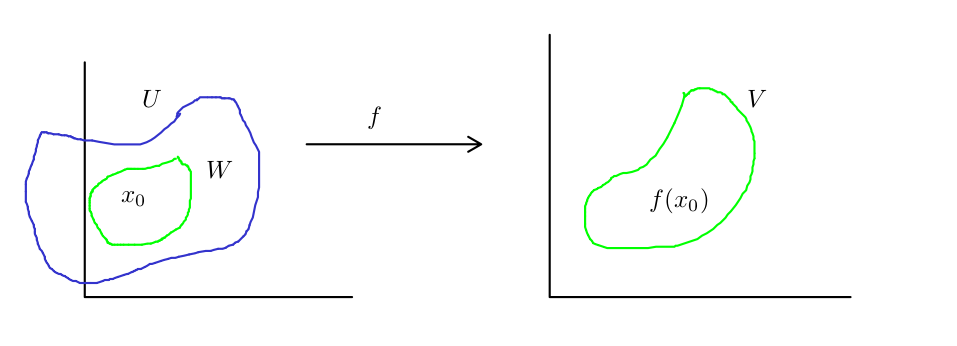
\includegraphics[scale=0.3]{figures/fct_inv.png}
  \caption{Fonctions inversibles}
  \label{}
\end{figure}

\begin{remark}
  Si en plus $f$ est de classe $\mathcal{C}^r$, alors $(f _{|W}) ^{-1} $ est aussi de classe $\mathcal{C}^r$.
\end{remark}

Notons que $\forall y \in V, x \in W, f(x)=y$,

\begin{gather*}
  (D(f _{|W})^{-1} )(y) = (Df(x)) ^{-1}.
\end{gather*}

En particulier, il existe $W$ tel que $Df(x)$ est inversible pour tout $x \in W$.

\subsection{Théorème du rang}\marginnote{20-09-2023}




\begin{thm}[Du rang]
  Soit $f : U \to \mathbb{R}^m$ (avec $U \subset \mathbb{R}^n$ de classe $\mathcal{C}^r, r \geq 1$).  Supposons que $\forall x \in U$,

  \[
  \operatorname{rang}(Df(x)) \equiv k,
  \]

  où $1 \leq k \leq m$ est fixé.

  $(Df(x) : \mathbb{R}^n \to \mathbb{R}^m, \text{ donc } 0 \leq \operatorname{rang}(Df(x)) \leq m)$.

  Soit $x_0 \in U$. Alors il y a des ouverts $W \subseteq \mathbb{R}^n, V \subseteq \mathbb{R}^m \text{ tels que }  x_0 \in W, f(x_0) \in V$ et 2 applications de classe $\mathcal{C}^r$ inversibles

\[
\begin{matrix}
  \varphi : W \to W' \text{ avec } W' \subseteq \mathbb{R}^n \text{ telle que } \varphi(x_0) =0 \\
  \psi : V \to V' \text{ avec } V' \subseteq \mathbb{R}^m \text{ telle que }  \psi(f(x_0)) = 0
\end{matrix}
\]
 telles que $\forall z \in W', z=(z_1, \dots, z_n)$,

  \[
  \psi \circ f \circ \varphi ^{-1} (z_1,z_2, \dots, z_n) = (z_1, z_2, \dots, z_k, 0, \dots, 0).
  \]
\end{thm}

\begin{figure}[h!]
  \centering
  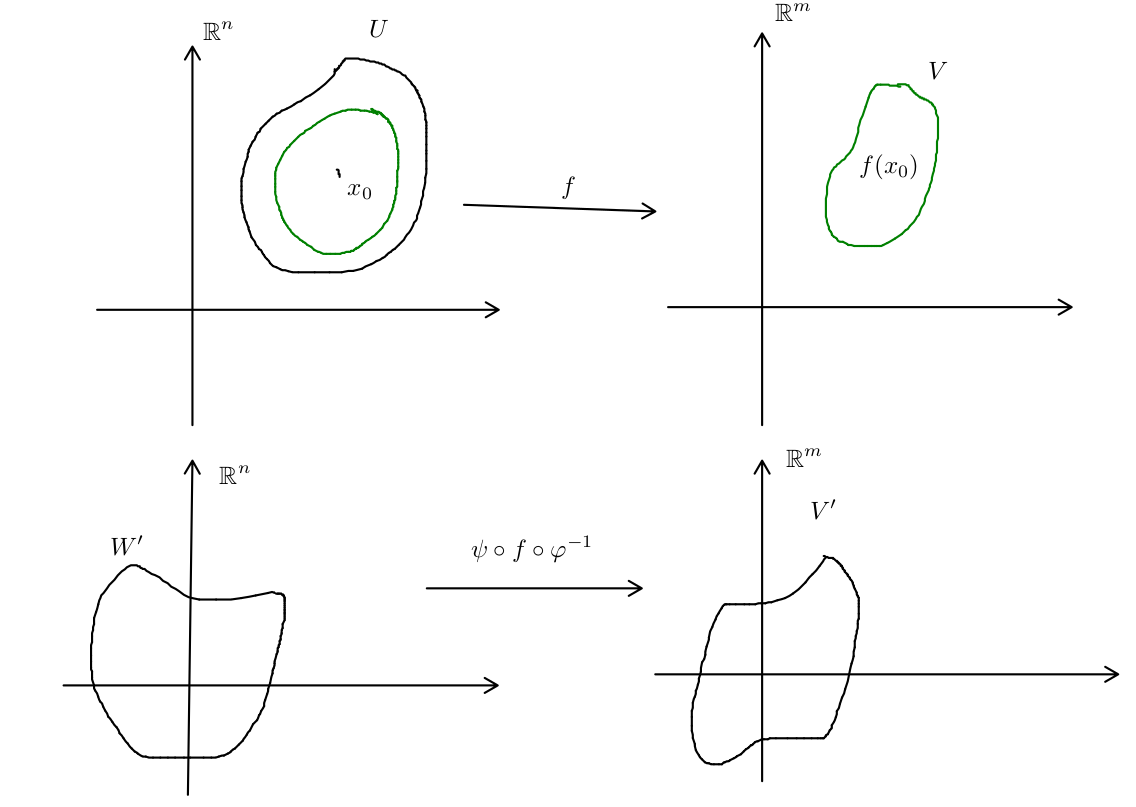
\includegraphics[scale=0.3]{figures/thm-rang.png}
  \caption{Illustration du théorème de rang}
  \label{}
\end{figure}

En particulier, $f(W)$ est un objet de dimension $k$, de régularité $\mathcal{C}^r$ (Si $m=3, k=2, f(W)$ est une surface de classe $\mathcal{C}^r$) et pour tout $y \in f(W), f ^{-1} (y)$ est un objet de dimension $n-k$ de régularité $\mathcal{C}^r$.

On note que les deux applications $\varphi$ et $\psi$ sont de classe $\mathcal{C}^r$ et inversibles. On peut démontrer que dans ce cas-là, les inverses $\varphi ^{-1} $ et $\psi ^{-1} $ sont aussi de classe $\mathcal{C}^r$.

\[
D \varphi ^{-1} (y) = (D \varphi (\varphi ^{-1} (y))^{-1} ), y \in W'.
\]

$\varphi ^{-1} $ étant continue, $D \varphi$ étant continue, l'inverse d'une matrice étant continue tant que $\operatorname{det} \neq 0$, $\varphi$ est de classe $\mathcal{C}^1$ inversible $\implies \varphi ^{-1} $ est de classe $\mathcal{C}^1$.

\begin{definition}[Difféomorphisme]
  Soient $U, U' \subseteq \mathbb{R}^n$ ouverts.

  Si $\varphi : U \to U'$ est une application de classe $\mathcal{C}^r$, avec l'inverse $\varphi ^{-1} : U' \to U$ de classe $\mathcal{C}^r$, on dit que $\varphi$ est un difféomorphisme de classe $\mathcal{C}^r$.
\end{definition}

\begin{remark}[Le théorème de rang dans le cas spécial où $f$ est linéaire]
  Soit $L : \mathbb{R}^n \to \mathbb{R}^m$, $\operatorname{rang}(L) = k, 0 \leq k \leq m$, alors il existe deux bases $\alpha_n$ et $\beta_m$ pour $\mathbb{R}^n$ et $\mathbb{R}^m$ telles que

  \[
  [L] _{\alpha_n} ^{\beta_m} =  \left[\begin{matrix}
    1 & 0 & \dots & 0 \\
    0 & 1 & \dots & 0 \\
    \vdots & \vdots & \ddots & \vdots \\
    0 & 0 & \dots & 0
  \end{matrix}\right] _{m \times n}.
  \]

  (En exercice).
\end{remark}

\begin{corollary}\label{inj}
  $U \subseteq \mathbb{R}^n, f : U \to \mathbb{R}^m$, $f$ est $\mathcal{C}^r, r \geq 1$.

  Supposons que pour $x_0 \in U$, $Df(x_0)$ est injective. $Df(x_0) \in \mathscr{L}(\mathbb{R}^n, \mathbb{R}^m) $. Alors il existe un voisinage $W$ de $x_0$ tel que $f$ est injective sur $W$.
\end{corollary}

\begin{proof}
  Pour $x \in U,$

  \[
  Df(x) = \left[\begin{matrix}
    \frac{\partial f }{\partial x_1} & \dots & \frac{\partial f }{\partial x_n }
  \end{matrix}\right] _{m \times n}.
  \]

  Si $Df(x_0)$ est injective, $\operatorname{rang}(Df(x_0)) = n \ (m \geq  n)$. On obtient une sous-matrice de $Df(x)$ de taille $n \times n$ inversible.
\end{proof}



\begin{lemma}[D'algèbre linéaire]
  $A \in \mathbb{R} ^{m \times n}$. Alors $\operatorname{rang} A = n$ si et seulement si il existe une sous-matrice $B \in \mathbb{R} ^{n \times n}$ de $A$ telle que $\operatorname{det} B \neq 0$.

  %\[
  %\left[\begin{matrix}
  %  \overrightarrow{ v_1 } & \dots & \overrightarrow{ v_n }
  %\end{matrix}\right],
  %\]

  %$\overrightarrow{ v_j } \in \mathbb{R}^m $.

  (En exercice).
\end{lemma}

Alors sous les hypothèse du corollaire \ref{inj}, $\operatorname{rang}Df(x) \equiv n$ dans un voisinage $W$ de $x_0$, appliquant le théorème du rang

\[
\tilde{f} = \varphi \circ f \circ \varphi ^{-1} (z_1, \dots, z_n) = (z_1, \dots, z_n, 0, \dots, 0)
\]

qui est injectif.

\begin{corollary}
  Les mêmes hypothèses que dans le corollaire \ref{inj}.

  Si $Df(x_0)$ est surjective, alors il existe un voisinage ouvert $V \subseteq f(U)$ de $f(x_0)$ (c'est à dire $f(x_0)$ est un point intérieur de $f(U))$ tel que $f$ est surjective sur $V$.
\end{corollary}

Argument à travers l'observation de l'algèbre linéaire qui dit que si $\operatorname{rang}(A) = m, m \leq n, A \in \mathbb{R}^{m \times n}$, il  y a une sous-matrice $B \in \mathbb{R}^{m\times m}$ tel que $\operatorname{det}(B) \neq 0$.

Théorème de rang : $k=m \leq n$.

Les détails en exercice.

\subsection{Théorème de fonctions implicites}


\begin{thm}[De fonctions implicites]
  $U \subseteq \mathbb{R}^n, V \subseteq \mathbb{R}^m$, $F : U \times V \to \mathbb{R}^m$ une application $\mathcal{C}^r, r \geq 1$.

  $(x_0, y_0) \in U \to V$ donné.

  \[
  DF(x_0) \in \mathbb{R}^{m \times (m+n)}
  \]

  et

  \[
  DF(x_0) = \left[\begin{matrix}
    \frac{\partial F }{\partial x_1} & \dots &\frac{\partial F }{\partial x_n } & \mid & \frac{\partial F }{\partial y_1 } & \dots & \frac{\partial F }{\partial y_m }
  \end{matrix}\right] _{m \times (m+n)}.
  \]

  Pour tout $(x_0, y_0) \in U \times V, DyF(x_0, y_0) \in \mathbb{R}^{m \times m}$. Supposons que $DyF(x_0)$ est inversible. Alors il existe un voisinage $W$ de $x_0$ dans $U$ et une application $\mathcal{C}^r$ $f : W \to V$ telle que $f(x_0) = y_0$ et

  \[
  \forall x \in W, F(x, f(x)) = F(x_0, y_0).
  \]
\end{thm}

\begin{figure}[h!]
  \centering
  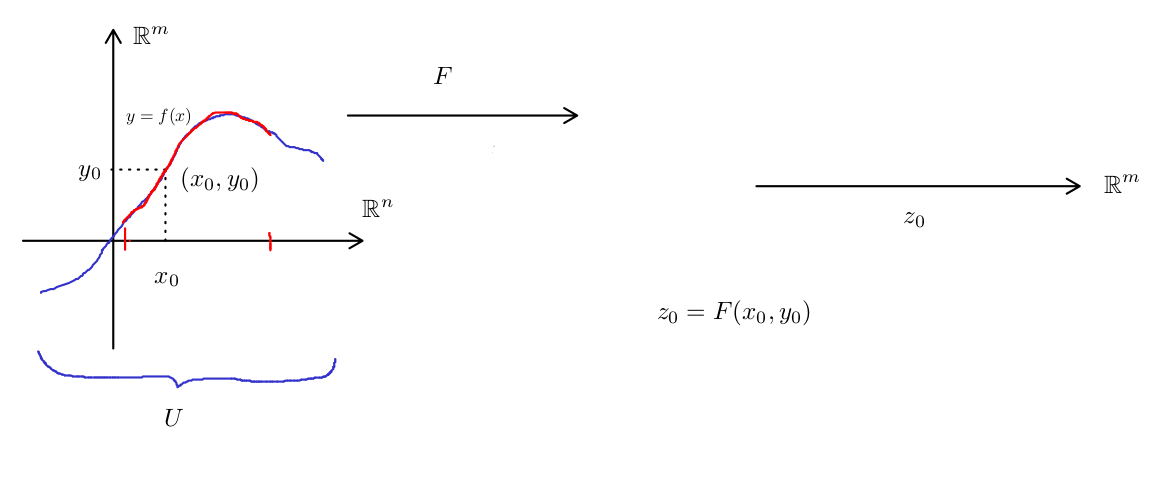
\includegraphics[scale=0.3]{figures/fct_impl.png}
  \caption{Illustration du théorème de fonctions implicites}
  \label{}
\end{figure}

Donc le graphe de $x \longrightarrow f(x)$ dans $W \times V$ pour l'application $f: W \to V$ est à l'intérieur de $F ^{-1} (x_0)$.

On peut dire que la fonction implicite

\[
F(x,y) = z_0, x \in \mathbb{R}^n, y \in \mathbb{R}^m, z_0 \in \mathbb{R}^n
\]

peut être exprimée explicitement $y = f(x)$ dans un voisinage $W$.

\paragraph{Exemple}

$m=1=n$.

Si $F(x, y) = y ^2-x$.

\subparagraph{Exemple 1} $x_0 = 0, y_0 =1 , z_0 =1$.

\[
DF = \left[\begin{matrix}
  \frac{\partial F }{\partial x} & \frac{\partial F }{\partial y }
\end{matrix}\right] = \left[\begin{matrix}
  -1 & 2y
\end{matrix}\right] \in \mathcal{C}^\infty.
\]

\[
DyF = [2y] _{|x|}.
\]

\[
DyF(x_0, y_0) = 2 y_0 = 2 \neq 0.
\]

Donc près de $(0, 1) = (x_0, y_0), y= f(x)$ a une solution $\mathcal{C} ^{\infty}$.

Mais si $x_0 = 0, y_0 = 0, z_0 = 0$, $DyF(x_0, y_0)=2y_0=0$ n'est pas inversible. $F$ est $\mathcal{C}^\infty$.

Implicitement, près de $(0, 0)$, on a $y ^2 - x = 0$.

On essaie de trouver $y=f(x)$.

$y ^2 = x \implies y = \pm \sqrt{ x } $.

Mais $\sqrt{\cdot} $ n'est pas définie pour $x \less 0$ près de $x_0 = 0$!

Donc il n'y a pas un moyen d'écrire explicitement $F(x,y) = 0$ près de $(0, 0)$ comme une fonction $\mathcal{C}^\infty$.

\begin{remark}[Sur le théorème des fonctions implicites]
  En effet, si $W' = f(W) \subset V$, on a

  \[
  (x,y) \in W \times W', F(x,y) = z_0 \iff y=f(x).
  \]
\end{remark}

\section{Algèbre multilinéaire}

Soit $E$ espace vectoriel sur $\mathbb{R}$ de dimension finie $n$, c'est-à-dire il existe $\beta = \{ \overrightarrow{ v_1 }, \dots, \overrightarrow{ v_n }   \} $ base telle que

\[
\forall \overrightarrow{ v } \in E, \exists ! (\alpha_1, \dots, \alpha_n), \overrightarrow{ v } = \sum_{i=1}^{n} \alpha_i \overrightarrow{ v_i }.
\]

En particulier, $\beta $ engendre $E$ ($E = \operatorname{span}(\beta) = \langle \beta \rangle $) si $\beta$ est libre.

\subsection{L'espace dual $E ^{*}$}

\[
E ^{*} = \{ T : E \to \mathbb{R} \text{ linéaire}  \} = \mathscr{L}(E, \mathbb{R}) .
\]


\begin{thm}
  On a $\operatorname{dim}(E ^{*}) = \operatorname{dim}(E)$.
\end{thm}

\begin{proof}
  Supposons $\beta = (e_1, \dots, e_n) $ est une base ordonnée de $E$. On définit alors $n$ éléments $(e ^{1}, e ^2, \dots, e ^{n})$, $e ^{j} \in E ^{*}$ de la manière suivante :

  \[
  e ^{j}(e_i) = \delta _{i} ^{j} = \begin{cases}
    1 \text{ si } i=j \\
    0 \text{ sinon. }
  \end{cases}
  \]

  \begin{remark}[Personnelle]
    $e ^{j}$ est l'évaluation du vecteur $\overrightarrow{ v } \in E$ en $e_j$.
  \end{remark}

  Donc $\displaystyle e ^j \left(\sum_{i=1}^{n} \alpha_i e_i \right) = \sum_{i=1}^{n} \alpha_i e ^{j}(e_i) = \sum_{i=1}^{n} \alpha_i \delta _{i} ^{j} = \alpha_i   $.

  Donc $\forall j \in \{ 1, \dots, n \}, e ^{j} \in E ^{*} $, $\beta ^{*} = \{ e ^{1}, \dots, e ^{n} \} $. On montre que $\beta ^{*}$ est une base pour $E ^{*}$.

  \begin{enumerate}
    \item $\beta ^{*}$ est libre. Supposons que pour $c_j \in \mathbb{R}$,

    \[
    \sum_{j=1}^{n} c_j e ^{j} = 0 \in E ^{*}.
    \]



    Donc pour tout $i$,
    \begin{gather*}
      \left(\sum_{j=1}^{n} c_j e ^{j} \right) (e_i) = 0 \in \mathbb{R} \text{ et } \\
      \left(\sum_{j=1}^{n} c_j e ^{j} \right) (e_i) = \sum_{j=1}^{n}c_j e ^{j}(e_i) = \sum_{j=1}^{n}c_j \delta_i ^{j} = c_i.
    \end{gather*}

    Donc $\forall i, c_i = 0$.

    \item $\beta ^{*}$ engendre $E ^{*}$. Soit $T \in E ^{*}$. Est-ce qu'il existe $\alpha_1,\dots, \alpha_n$ tel que

    \[
    T = \sum_{j=1}^{n} \alpha_j e ^{j} \ ?
    \]

    Essayons de trouver les $\alpha_j$ en appliquant l'identité desirée en $e_i$.

    \begin{gather*}
      \forall i, T(e_i) = \left( \sum_{j=1}^{n} \alpha_j e_j \right)(e_i) = \sum_{j=1}^{n} \alpha_j e_j(e_i) = \sum_{j=1}^{n} \alpha_j \delta_i ^{j} = \alpha_i.
    \end{gather*}

    Donc pour $T \in E ^{*}$ donnée, le candidat pour $\alpha_i$ est

    \[
    \forall i \in \{ 1, \dots, n \}, \alpha_i \in T(e_i) \in \mathbb{R},
    \]

    et on obtient que

    \[
    \forall i \in \{ 1, \dots, n \}, T(e_i) = \left(\sum_{j=1}^{n} \alpha_j e ^{j} \right) (e_i).
    \]

    Comme $T$ et $\tilde{T}$ ont les mêmes valeurs sur la base $\beta $, donc $T = \tilde{T}$.

    \[
    T = \sum_{j=1}^{n} T(e_j) e ^{j}.
    \]

  \end{enumerate}
\end{proof}


\begin{definition}
  On dit que $\beta ^{*}$ est la base duale de $\beta $.
\end{definition}

On considère le dual du dual $E ^{**} = (E ^{*}) ^{*}$.


\begin{thm}
  Si $\operatorname{dim}(E) \less \infty$, il y a un isomorphisme canonique entre $E$ et $E ^{**}$.
\end{thm}

On peut définir $E \to E ^{**}$. On pose $e : E \to E ^{**}$.

\[
(\iota(\overrightarrow{ v } ))(T) = T(\overrightarrow{ v } ),
\]

$\forall T \in E ^{*} = \mathscr{L}(E, \mathbb{R}) $.

\begin{exo}

  \

  \begin{enumerate}
    \item Montrer que $\forall v \in E, \iota(\overrightarrow{ v } ) : E ^{*} \to \mathbb{R}$ est une transformation linéaire.
    \item Montrer que $\iota : E \to E ^{**}$ est une transformation linéaire.
    \item Montrer que $\iota$ est bijective (donc un isomorphisme).
  \end{enumerate}
\end{exo}

\begin{proof}

  \

  \begin{enumerate}
    \item \begin{gather*}
      \iota(\overrightarrow{ v } ) (\alpha T+ S) = (\alpha T+S)(\overrightarrow{ v } ) = \alpha T(\overrightarrow{ v } )+ S(\overrightarrow{ v } ) = \alpha \iota(\overrightarrow{ v } )(T)+ \iota(\overrightarrow{ v } )(S).
  \end{gather*}
    \item $\iota : E \to E ^{**}$ est linéaire.

    \begin{gather*}
      \iota(\alpha \overrightarrow{ v } + \overrightarrow{ w }  )(T) = T(\alpha \overrightarrow{ v } + \overrightarrow{ w } ) \stackrel{T \text{ linéaire} }{=} \alpha T(\overrightarrow{ v } )+ T(\overrightarrow{ w } ) \\
      = \alpha \iota(\overrightarrow{ v } )(T)+ \iota(\overrightarrow{ w } ) (T) = \alpha \iota (\overrightarrow{ v } )+ \iota(\overrightarrow{ w }).
    \end{gather*}

    Comme c'est vrai $\forall T \in E ^{*}$, on a l'identification $\iota(\alpha \overrightarrow{ v }+ \overrightarrow{ w }  ) = \alpha \iota(\overrightarrow{ v } )+ \iota(\overrightarrow{ w } )$ (comme un élément de $E ^{**}$). Donc $\iota$ est une transformation linéaire.

    \item On sait que $dim E = dim E ^{*} = dim E ^{**}$ (ce qui veut dire que $\iota$ est surjective). Pour démontrer que $\iota$ est un isomorphisme, il suffit de démontrer que $\operatorname{Ker}(\iota) = \{ 0 \} $ (que $\iota$ est injective).

    Si $\overrightarrow{ v }  \in \operatorname{Ker}(\iota)$, alors $\iota(\overrightarrow{ v } ) = 0 \implies \forall T \in E ^{*}, T(\overrightarrow{ v } ) = \iota(\overrightarrow{ v })(T) = 0(T) =0$, donc $\overrightarrow{ v } $ est tel que $\forall T \in E ^{*}, T(\overrightarrow{ v } ) =0$.

    Si $\overrightarrow{ v } \neq \overrightarrow{ 0 }  $, on peut compléter $\overrightarrow{ v } $ avec une base $\{ \overrightarrow{ v }, \overrightarrow{ v_2 },\dots, \overrightarrow{ v_n } \} $ de $E$ et définir $T(\alpha_1 \overrightarrow{ v } + \alpha_2 \overrightarrow{ v_2 } + \dots + \alpha_n \overrightarrow{ v_n }  ) = \alpha_1$. Dans ce cas-là, $T(\overrightarrow{ v } ) = 1 \neq 0$.

    Si $\beta = (e_1, \dots, e_n)$ base de $E$. On a vu que la base duale $\beta ^{*} = (e ^{1}, e ^2, \dots, e ^{n})$ est une base de $E ^{*}$.

    \[
    e ^{j}(e_i) = \delta_i ^{j}.
    \]

    \[
    (\beta ^{*}) ^{*} = \beta ^{**} = (\varepsilon_1, \eta_2, \dots, \eta_n).
    \]

    \begin{equation} \label{base1}
      \forall i, \eta_i \in E ^{**}, \eta_i(e ^{i}) = \delta_i ^{j}, \forall i, j.
    \end{equation}

    On va aussi calculer

    \begin{equation} \label{base2}
      \iota(e_i)(e ^{j}) = e ^{j}(e_i) = \delta_i ^{j}.
    \end{equation}

    $\forall e ^{j}$ de base $\beta ^{*}$, on a

    \[
    \eta_i(e ^{j}) = \iota(e_i)(e ^{j}), \eta_i, \iota(e_i) \in E ^{**} = \mathscr{L}(E ^{*}, \mathbb{R}).
    \]

    $\eta _i$ et $i(e_i)$ coincident sur une base de $E ^{*}$, donc

    \[
    \forall i, \eta_i = \iota(e_i).
    \]

    Pour simplifier, parfois on identifie $E$ et $E ^{**}$ par l'application $\iota$, c'est-à-dire on met $\overrightarrow{ v } = \iota(\overrightarrow{ v })$.
  \end{enumerate}
\end{proof}

Les éléments de $E ^{*}$ sont appelés \textbf{les vecteurs covariants}. Les éléments de $E ^{**}$ sont appelés \textbf{les vecteurs contravariants}.

\subsection{Les applications multilinéaires}

Supposons que $E_1, E_2, \dots, E_k$ sont des espaces vectoriels sur $\mathbb{R}$ et $E'$ espace vectoriel de $\mathbb{R}$.

\[
\alpha : E_1 \times E_2 \times \dots \times E_k \longrightarrow E'
\]

est une application $k$-linéaire quand $\alpha$ est linéaire par rapport à chaque coordonnée dans l'un des espaces $E_j$ quand les autres coordonnées (composantes) sont fixées.

$\overrightarrow{ v_i } \in E_i $, $1 \leq i \leq k$, $\alpha(\overrightarrow{ v_1 }, \overrightarrow{ v_2 }, \dots, \overrightarrow{ v_k })$.

Si $\forall i \in \{ 1, \dots, k \}$, $a \in \mathbb{R}, \forall \overrightarrow{ v_j } \in E_j, \overrightarrow{ w } \in E_i $, on a

\[
\alpha(\overrightarrow{ v_1 }, \overrightarrow{ v_2 }, \dots, a \overrightarrow{ v_i }+ \overrightarrow{ w }, \dots, \overrightarrow{ v_k }) = a \alpha(\overrightarrow{ v_1 }, \dots, \overrightarrow{ v_i }, \dots, \overrightarrow{ v_k })+ \alpha(\overrightarrow{ v_1 }, \overrightarrow{ v_2 }, \dots, \overbrace{\overrightarrow{ w } }^{i\text{-ème}}, \dots, \overrightarrow{ v_k }).
\]

\paragraph{Exemple}

\begin{enumerate}
  \item $f(x,y) = xy$, $f : \stackrel{E_1}{\mathbb{R}} \times \stackrel{E_2}{\mathbb{R}} \to \stackrel{E'}{\mathbb{R}}$.
  \item $E_1 = E_2 = \mathbb{R}^n$, $E' = \mathbb{R}$,

  \[
  \alpha(\overrightarrow{ v_1 }, \overrightarrow{ v_2 } ) = \overrightarrow{ v_1 }\cdot \overrightarrow{ v_2 } \text{ 2-linéaire. }
  \]

  \item $E_1 = E_2 = E_3 \equiv \mathbb{R}^3$, $E' = \mathbb{R}$.
  \[
  \alpha(\overrightarrow{ v_1 }, \overrightarrow{ v_2 }, \overrightarrow{ v_3 }) = \overrightarrow{ v_1 } \cdot (\overrightarrow{ v_2 } \wedge \overrightarrow{ v_3 }  ) = det \left( \left[\begin{matrix}
  \overrightarrow{ v_1 } \\
  \overrightarrow{ v_2 }  \\
  \overrightarrow{ v_3 }
  \end{matrix}\right]\right)  _{3 \times 3}.
  \]

  Cette application est 3-linéaire.

  \item $E_1 = E_2 = \dots = E_n = \mathbb{R}^n$.

  \[
  \alpha(\overrightarrow{ v_1 }, \overrightarrow{ v_2 }, \dots, \overrightarrow{ v_n } ) = det \left(\left[\begin{matrix}
  \overrightarrow{ v_1 } \\
  \overrightarrow{ v_2 } \\
  \vdots \\
  \overrightarrow{ v_n }
  \end{matrix}\right]\right).
  \]

  C'est une application $n$-linéaire.

  \item Le déterminant d'une matrice de taille $n \times n$ est une application $n$-linéaire.
\end{enumerate}




\subsubsection{Quelques notations}

$E$ espace vectoriel de dimension finie.

On note $\Omega ^{k}(E) := \{ \alpha : \underbrace{E \times E \times \dots \times E}_{k \text{ fois} }  \to \mathbb{R} \mid \alpha \text{ est } k \text{-linéaire}  \} $.

Remarquons que $\Omega ^{1}(E) = \{ \alpha : E \to \mathbb{R} \mid \alpha \text{ est linéaire}  \} = E ^{*}$.

\begin{prop}
  $\forall k \in \mathbb{N} ^{*}, \Omega ^{k}(E) $ est un espace vectoriel de dimension $n ^{k}$.
\end{prop}

\begin{proof}
  Si $\alpha, \beta \in \Omega ^{k}(E), a \in \mathbb{R}$. Pour montrer que \(\Omega ^{k}(E)\) est un espace vectoriel de dimension \(n ^{k}\), on doit montrer deux choses :

  \begin{enumerate}
    \item \(\Omega ^{k}(E)\) est stable par les opérations + et \(\cdot\) (produit par un scalaire).
    \item Il existe une base de cet espace contenant \(n ^{k}\) éléments.
  \end{enumerate}

   Il faut démontrer que $a \alpha+ \beta$ est aussi une application $k$-linéaire sur $E ^k = \overbrace{E \times \dots \times E}^{k \text{ fois}}$.

  \begin{gather*}
    (a \alpha + \beta)(b \overrightarrow{ v_1 }+ \overrightarrow{ w }, \dots) = a[\alpha(b \overrightarrow{ v_1 }+ \overrightarrow{ w }, \dots)]+ \beta(b \overrightarrow{ v_1 }+\overrightarrow{ w })\\
    = a[b \alpha(\overrightarrow{ v_1 }, \dots)+ \alpha(\overrightarrow{ w }, \dots)] + b \beta(v_1, \dots) + \beta(\overrightarrow{ w }, \dots) \\
    = b[a \alpha+ \beta](\overrightarrow{ v_1 }, \dots )+ [a \alpha+ \beta](\overrightarrow{ w }, \dots)
  \end{gather*}

  De même pour chaque $1 \leq i \leq k$.

  Pour trouver la dimension de $\Omega ^{k}(E)$, il faudra trouver une base de $\Omega ^{k}(E)$. Pour cela, il faudra d'abord introduire ``le produit tensoriel''.
\end{proof}

\begin{definition}[Produit tensoriel]
  Supposons que $\alpha : E_1 \times \dots \times E_k \to \mathbb{R}$ $k$-linéaire, $\beta: E_1' \times \dots \times E_l' \to \mathbb{R}$ $l$-linéaire.

  On définit

  \[
  \alpha \otimes \beta : E_1 \times \dots \times E_k \times E_1' \times \dots \times E_l' \longrightarrow \mathbb{R}
  \]

  telle que

  \[
  \alpha \otimes \beta(\overrightarrow{ v_1 }, \dots, \overrightarrow{ v_k }, \overrightarrow{ v_1' }, \dots, \overrightarrow{ v_l'} ):=\alpha(\overrightarrow{ v_1 }, \dots, \overrightarrow{ v_k }) \beta(\overrightarrow{ v_1' }, \dots, \overrightarrow{ v_l'})
  \]

  qui est une application $(k+l)$-linéaire (avec $\overrightarrow{ v_i } \in E_i, i \in \{ 1, \dots, k \}, \overrightarrow{ v_j' } \in E_j', j \in \{ 1, \dots, l\}$).
\end{definition}

Les applications $k$-linéaires sont appelées les tenseurs covariants d'ordre $k$.

\begin{exo}
  On montre que $\otimes$ est une opération associative.

  $\forall \alpha, \beta, \gamma $ tenseurs covariants,

  \[
  (\alpha \otimes \beta) \otimes \gamma = \alpha \otimes (\beta \otimes \gamma ).
  \]
\end{exo}

\paragraph{Exemple} $E_1 = \mathbb{R}^{n}, E_1' = \mathbb{R} ^{n}, k=l=1, \alpha \in E_1 ^{*}, \alpha(\overrightarrow{ v }) =2 \overrightarrow{ v } \cdot e_1  , \forall \overrightarrow{ v } \in \mathbb{R}^n, \beta \in E_1^{'*}, \beta (\overrightarrow{ v' } ) = \overrightarrow{ v' } \cdot e_1, \forall \overrightarrow{ v' } \in \mathbb{R}^n$.

\[
\alpha \otimes \beta(\overrightarrow{v}, \overrightarrow{ v' }) = 2 (\overrightarrow{ v }\cdot e_1)(\overrightarrow{ v' } \cdot e_1)
\]

et

\[
\beta \otimes \alpha(\overrightarrow{ v' }, \overrightarrow{ v } ) = 2(\overrightarrow{ v' }\cdot e_1 )(\overrightarrow{ v } \cdot e_1 ).
\]

Mais si $\tilde{\beta}(\overrightarrow{ v' } ) = \overrightarrow{ v' } \cdot e_2 $,

\begin{gather*}
  \alpha \otimes \tilde{\beta} (\overrightarrow{ v }, \overrightarrow{ v' }) = 2 (\overrightarrow{ v } \cdot e_1 )(\overrightarrow{ v' }\cdot e_2 ), \\
  \text{mais } \tilde{\beta }\otimes \alpha(\overrightarrow{ v' }, \overrightarrow{ v }  ) = 2 (\overrightarrow{ v' }\cdot e_1 )(\overrightarrow{ v }\cdot e_2 ).
\end{gather*}

Le produit tensoriel n'est donc pas commutatif.

\

$E ^{k} = \underbrace{E \times \dots \times E}_{k \text{ fois} }$

$\Omega ^{k}(E) := \{ \alpha : \underbrace{E \times E \times \dots \times E}_{k \text{ fois} }  \to \mathbb{R} \mid \alpha \text{ est } k \text{-linéaire}  \} $.

\begin{prop}\label{dim-tens}
  $\Omega ^{k}(E)$ est un espace vectoriel de dimension $n ^k$, où $n = dim(E)$.
\end{prop}

\begin{proof}
  On rappelle que $\operatorname{dim}(E) = n$, que $(e_1, \dots, e_n)$ est une base de $E$ et que $(e ^{1}, \dots, e ^{n})$ est une base de $E ^{*} = \Omega ^{1}(E)$.

  Par exemple si on prend

  \[
  \underbrace{e^{1} \otimes e ^{1} \otimes \dots \otimes e ^{1}}_{k \text{ fois} } : E \times \dots \times E \to \mathbb{R},
  \]

  on aura alors

  \begin{gather*}
    e^{1} \otimes e ^{1} \otimes \dots \otimes e ^{1}(\overrightarrow{ v_1 }, \dots, \overrightarrow{ v_n }  ), \overrightarrow{ v_i } \in E, \\
    = e ^{1}(\overrightarrow{ v_1 } ) e ^{1}(\overrightarrow{ v_2 } ) \dots e ^{1}(\overrightarrow{ v_n }).
  \end{gather*}

  Posons $\mathscr{A} = \{ e ^{i_1} \otimes e ^{i_2} \otimes \dots \otimes e ^{i_k} \mid \text{pour } 1 \leq j \leq k, 1 \leq i_k \leq n  \} $.

  Il y a $n$ choix pour chaque $e ^{i_j}$ (parmi les \(n\) vecteurs de la base de \(E\)), alors, au total, on a $n^k$ choix pour les éléments de $\mathscr{A}$ (puisqu'il y a \(k\) choix pour chaque \(i_k\)), ce qui démontre la proposition \ref{dim-tens}. Il nous reste maintenant à montrer que :

  \begin{enumerate}
    \item $\mathscr{A} $ engendre $\Omega ^{k}(E)$ ;
    \item $\mathscr{A} $ est libre.
  \end{enumerate}

  Soit $\alpha \in \Omega ^{k}(E)$.

  On va démontrer que

  \[
  \alpha \stackrel{?}{=} \sum_{1 \leq i_1, \dots, i_k \leq n}^{} \alpha(e _{i_1}, e _{i_2}, \dots, e _{i_k}) e ^{i_1} \otimes e ^{i_2} \otimes \dots \otimes e ^{i_k}.
  \]

  Prenons $(\overrightarrow{ v_1 }, \overrightarrow{ v_2 }, \dots, \overrightarrow{ v_n }) \in E ^{k}$. On a

  \begin{gather*}
    \overrightarrow{ v_j } = \sum_{i=1}^{n} c _{ij} e_i.
  \end{gather*}

  \begin{gather*}
    \alpha(\overrightarrow{ v_1 }, \dots, \overrightarrow{ v_k }) = \alpha\left(\sum_{i=1}^{n}c _{i1}e_i, \dots, \sum_{i=1}^{n} c _{ik} e_i\right) \\
    = \sum_{i=1}^{n} c _{i1} \alpha\left(e_i, \sum_{i_2}^{} c _{i_2 2} e _{_2 i}, \dots  \right)  \\
    = \sum_{i_1 =1}^{n} \sum_{i_2=1}^{n} \dots \sum_{i_k=1}^{n} c _{i_1 1} c _{i_2 2} \dots c _{i_k k} \alpha(e _{i_1},\dots, e _{i_k}).
  \end{gather*}

  Maintenant, pour

  \[
  \beta = \sum_{1 \leq i_1, \dots, i_n \leq n}^{} \alpha(e_{i_1}, \dots,  e_{i_n}) e ^{i_1}\otimes \dots \otimes e ^{i_n},
  \]

  on calcule pour $\beta  \in \Omega ^{k}(E)$,

  \begin{gather*}
    \beta (\overrightarrow{ v_1 }, \dots, \overrightarrow{ v_k })= \sum_{i_1}^{} \sum_{i_2}^{} \dots \sum_{i_k}^{} c _{i_1} c _{i_2} \dots c _{i_k} \beta(e _{i_1}, \dots, e _{i_n}).
  \end{gather*}

  Mais

  \begin{gather*}
    \beta (e _{i_1}, \dots, e _{i_k}) = \sum_{1 \leq i_1', \dots, i_k' \leq n}^{} \alpha( e _{i_1'}, e _{i_2'}, \dots, e _{i_k'}) e ^{i_1'}\otimes e ^{i_2'} \otimes \dots \otimes e ^{i_k'} (e_{i_1},\dots, e_{i_k}) \\
    = \sum_{1 \leq i_1' \leq \dots \leq i_k' \leq n}^{} \alpha(e _{i_1'}, \dots, e _{i_k'}) e ^{i_1'}(e _{i_1}) e ^{i_2'}(e _{i_2}) \dots e ^{i_k'} (e _{i_k}) \\
    =\sum_{1 \leq i_1', \dots, i_k' \leq n}^{} \alpha(e _{i_1'}, \dots, e _{i_k'}) \delta _{i_1} ^{i_1'} \dots \delta _{i_k} ^{i_k'} = \alpha(e _{i_1}, \dots, e _{i_n}).
  \end{gather*}

  Donc

  \begin{gather*}
    \beta (\overrightarrow{ v_1 }, \dots, \overrightarrow{ v_k }  ) = \sum_{i_1}^{} \sum_{i_2}^{} \dots \sum_{i_k}^{} c _{i_1 1} c _{i_2 2} \dots c _{i_k k} \alpha(e _{i_1}, \dots, e _{ik}) = \alpha(\overrightarrow{ v_1 }, \dots, \overrightarrow{ v_k }  )   .
  \end{gather*}

  Donc ? est démontré, et on a $\alpha \in span(\mathscr{A} ) = \langle \mathscr{A} \rangle $, où $\mathscr{A} = \{ e ^{i_1} \otimes \dots \otimes e ^{i_k}\} $.

  \

  Montrons que $\mathscr{A} $ est libre. Soit

  \begin{gather*}
    \sum_{1 \leq i_1 , \dots, i_k \leq n}^{} c _{i_1 i_2 \dots i_k}  e ^{i_1} \otimes \dots \otimes e ^{i_k} = 0 \in \Omega ^{k}(E).
  \end{gather*}

  Le même calcul qu'auparavant démontre que

  \[
  0 = 0(e _{i_1}, \dots, e _{i_k}) = c _{i_1 \dots i_k}, \forall i_1, \dots, i_k,
  \]

  donc

  \[
  \forall i_1, \dots, i_k, c _{i_1 \dots i_k} =0,
  \]

  donc $\mathscr{A} $ est libre.
\end{proof}

\begin{remark}
  Si $f : U \to \mathbb{R}^m, U \subseteq \mathbb{R}^n$, $Df(x) \in \mathscr{L}(\mathbb{R}^n, \mathbb{R}^m) $,

  \begin{gather*}
    Df:U \to \mathscr{L}(\mathbb{R}^n, \mathbb{R}^n) \\
    D ^2 f(x) \in \mathscr{L}(\mathbb{R}^n, \mathscr{L}(\mathbb{R}^n, \mathbb{R}^m) ) \\
    \vdots \\
    D ^{n}f(x) \in \mathscr{L}(\mathbb{R}^n, \mathscr{L}(\mathbb{R}^n, \dots, \mathscr{L}(\mathbb{R}^n, \mathbb{R}^m) ) ) .
  \end{gather*}
\end{remark}

\begin{lemma}
  $\mathscr{L}(\mathbb{R}^n, \mathscr{L}(\mathbb{R}^n, \mathbb{R}^m) ) \simeq \{ \alpha : \mathbb{R}^n \times \mathbb{R}^n \to \mathbb{R}^n \mid \alpha \text{ est 2-linéaire} \}  $.
\end{lemma}

Pour un élément $g \in \mathscr{L}(\mathbb{R}^n, \mathscr{L}(\mathbb{R}^n, \mathbb{R}^m) ) $ et $\overrightarrow{ v } \in \mathbb{R}^n, g(\overrightarrow{ v } ) \in \mathscr{L}(\mathbb{R}^n, \mathbb{R}^m) $.

Pour tout $k$, pour tout $x \in U$, $D ^{k}f(x) \in (\Omega ^{k}(\mathbb{R}^n))^{m}$. Cet espace est de dimension $m(n ^{k})$.

On définit

\[
\alpha_g(\overrightarrow{ v } )(\overrightarrow{ w } ) \in \mathbb{R}^n.
\]

On voit que $\alpha _{g}$ est une application 2-linéaire.

Supposons que $\alpha_g = \alpha _{g'}, $ donc $ \forall \overrightarrow{ v }, \overrightarrow{ w } \in \mathbb{R}^n, \alpha _{g}(\overrightarrow{ v }, \overrightarrow{ w }) = \alpha _{g'}(\overrightarrow{ v }, \overrightarrow{ w }) $, donc $g(\overrightarrow{ v } )(\overrightarrow{ w } ) = g'(\overrightarrow{ v } )(\overrightarrow{ w } )$.

Donc $\forall \overrightarrow{ v } \in \mathbb{R}^n, g(\overrightarrow{ v } ) = g'(\overrightarrow{ v } ) \in \mathscr{L}(\mathbb{R}^n, \mathbb{R}^m)$, donc $g = g'$.

On en déduit que $g \longrightarrow \alpha_g$ est injective.



\begin{exemple}\marginnote{27-09-2023}
  \(T : \mathbb{R}^2 \to \mathbb{R}, Tx =  2x_1+ 5x_2 \). On définit \(\alpha : \mathbb{R}^2 \times \mathbb{R}^2 \to \mathbb{R}\), \(\alpha((x_1, x_2), (x_1', x_2')) = x_1 x_2'-x_2 x_1', \alpha \in \Omega ^2(\mathbb{R}^2)\).

  Ecrire le produit tensoriel entre \(\alpha\) et \(T\)...
\end{exemple}

Si \(E, F\) sont deux espaces vectoriels et \(T : E \longrightarrow F\) linéaire (\(T \in \mathscr{L}(E, F) \)). On peut définir une application linéaire

\[T ^{*} : F ^{*} \longrightarrow E ^{*}.\]

Pour \(f \in F ^{*}\), on doit déterminer \(T ^{*}(f)\) comme un élément de \(E ^{*}\). Alors \(T ^{*}(f)\) doit être une application linéaire \(T ^{*}(f) \in \mathscr{L}(E, \mathbb{R})\), i. e. \(T ^{*}(f) : E \longrightarrow \mathbb{R}\).

\[\forall v \in E, (T ^{*}(f))(v) \stackrel{\text{déf}}{=} f(T(v)) \text{ cf figure \ref{tstar}}. \]

On a \(f \in F ^{*}, f \in \mathscr{L}(F, \mathbb{R})\).

\begin{figure}[h!]
  \centering
  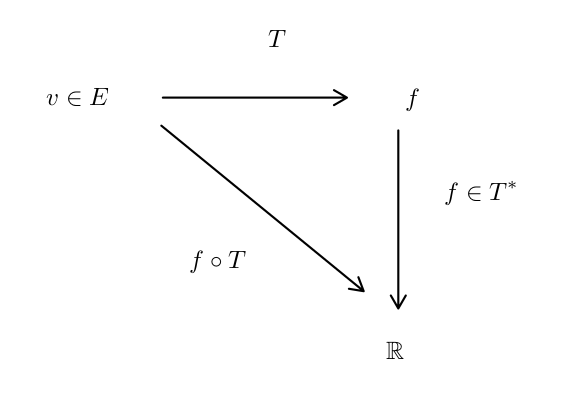
\includegraphics[scale=0.3]{figures/tstar.png}
  \caption{Illustration de \(T ^{*}\)}
  \label{tstar}
\end{figure}

\(F ^{*} = \Omega'(F), E ^{*} = \Omega'(E)\). On peut aussi utiliser la notation \(\Omega ^{1}(T)\) pour \(T ^{*}\). On peut aussi définir, à partir de \(T\),

\[\Omega ^{k}(T) : \underbrace{\Omega ^{k}(F)}_{\alpha}  \longrightarrow \underbrace{\Omega ^{k}(E)}_{\beta}.\]

Pour \(\alpha \in \Omega ^{k}(E)\), on a besoin que \( \underbrace{\Omega ^{k}(T)(\alpha)}_{k\text{-linéaire}} \in \Omega ^{k}(E)\).

\(\forall v_1, \dots, v_n\), on a besoin de définir

\[ \underbrace{(\Omega ^{k}(T))(\alpha)}_{\beta \in \Omega ^{k}(E)}(v_1, \dots, v_k) = \underbrace{\alpha(T(v_1), T(v_2), \dots, T(v_k))}_{\in F ^{k}}.\]


\begin{exo}

  \

  \begin{enumerate}
    \item Montrer que \(\beta\) est \(k\)-linéaire, i. e. \(\forall k , \Omega ^{k}(T)(\alpha) \in \Omega ^{k}(E)\).
    \item Montrer que \(\Omega ^{k}(S \circ T) = \Omega ^{k}(T) \circ \Omega ^{k}(S)\).
    \item Montrer que \(\Omega ^{k}(\mathds{1}_{E}) = \mathds{1}_{\Omega ^{k}(E)}\).
    \item Montrer que si \(T : E \to F\) est inversible, alors

    \[\Omega ^{k}(T ^{-1} ) = (\Omega ^{k}(T)) ^{-1}. \]
  \end{enumerate}
\end{exo}

\paragraph{Quelques propriétés}

Si on a \(E \stackrel{T}{\longrightarrow} F \stackrel{S}{\longrightarrow} {G}\), on a \[\Omega ^{k}(G) \stackrel{\Omega ^{k}(S)}{\longrightarrow} \Omega ^{k}(F) \stackrel{\Omega ^{k}(T)}{\longrightarrow} \Omega ^{k}(E).\]

On a \(S \circ T : E \longrightarrow G\). Alors \[\Omega ^{k}(T) \circ \Omega ^{k}(S) \in \Omega ^{k}(G) \longrightarrow \Omega ^{k}(E)\] et \[\Omega ^{k}(S \circ T) : \Omega ^{k}(G) \longrightarrow \Omega ^{k}(E).\]

On considère \(\mathds{1}_{E} : E \to E\). Alors \[\Omega ^{k}(\mathds{1}_{E}) = \mathds{1}_{\Omega ^{k}(E)}.\]

\

On rappelle que l'on peut associer à un vecteur \(v \in E\) un vecteur contravariant \( \iota(v) \in E ^{**}\). On définit alors, \(\forall l \in \mathbb{N}, l \geq  1\),

\[\Omega _{l}(E) := \{ \alpha : \underbrace{E ^{*} \times \dots \times E ^{*}}_{k \text{ fois} } \to \mathbb{R} \mid \alpha \text{ est } l\text{-linéaire}\} = \Omega ^{l}(E ^{*}), \]

avec la base \(\{ e _{i_1} \otimes \dots \otimes e _{i_l} \mid 1 \leq i_j \leq  n, 1 \leq j \leq l \}\).

On a \(\operatorname{dim}(\Omega_{l}(E)) = n ^{l}\) et \( \forall \alpha \in \Omega _{l}(E)\),

\[\alpha = \sum_{1 \leq i_1, \dots, i_l \leq n}^{} \alpha(e ^{i_1}, \dots, e ^{i_l}) e _{i_1} \otimes \dots \otimes e _{i_l}.\]

Pour \( T : E \longrightarrow F\), \(\Omega _{l}(T) : \Omega _{l}(E) \to \Omega _{l}(F)\) (objets contravariants pour la dualité), avec \(\alpha \in \Omega _{l}(E), \beta = \Omega _{l}(T)(\alpha) \in \Omega _{l}(F)\).

On va essayer de définir

\[\beta \underset{f_j \in F ^{*}}{(f_1, \dots, f_l)} = \Omega _{l}(T)(\alpha)(f_1, \dots, f_l) \stackrel{\text{déf}}{=} \alpha \underset{T ^{*}(f_j) \in F ^{*}}{(T ^{*}(f_1), \dots, T ^{*}(f_l))}.\]

On a alors le schéma suivant :

\begin{gather*}
  E \stackrel{T}{\longrightarrow} F \stackrel{S}{\longrightarrow} G \\
  \Omega _{l}(E) \underset{\Omega _{l}(T)}{\longrightarrow}\Omega _{l}(F) \underset{\Omega _{l}(S)}{\longrightarrow} \Omega _{l}(G).
\end{gather*}


\begin{definition}
  Pour tous \( k, l\), on a

  \[\Omega ^{k} _{l}(E) := \{ \alpha : \underbrace{E \times \dots \times E}_{k \text{ fois}} \times \underbrace{E ^{*} \times \dots \times E ^{*}}_{l \text{ fois}} \mid \alpha \text{ est } k \text{-linéaire}\}\]

  qui a pour base

  \[\{ e ^{i_1} \otimes \dots \otimes e ^{i_k} \otimes e _{j_1} \otimes \dots \otimes e _{j_l} \mid 1 \leq i_1, \dots, i_k \leq n, 1 \leq j_1, \dots, j_l \leq n\}.\]
\end{definition}

On a \(\operatorname{dim}(\Omega ^{k} _{l}) = n ^{k+l}\). Pour \(\alpha \in \Omega _{l} ^{k}(E)\), on écrit

\[\alpha = \sum_{\substack{1 \leq i_1, \dots, i_k \leq n \\ 1 \leq j_1, \dots, j_l}}^{} \alpha(e _{i_1}, \dots, e _{i_k}, e ^{j_1}, \dots, e ^{j_l}) e ^{i_1} \otimes \dots \otimes e ^{i_k} \otimes e _{j_1} \otimes \dots \otimes e _{j_l}. \]

\paragraph{Parenthèse sur les notations}

En physique, on écrit

\[\alpha = \sum_{\substack{i_1, \dots, i_k \\ j_1, \dots, j_l}}^{} a _{i_1 \dots i_k} ^{j_1 \dots j_l} e ^{i_1} \otimes \dots e ^{i_k} \otimes e _{j_1} \otimes \dots \otimes e ^{j_l}. \]

et on dit : si \(\alpha\) est un \((l, k) \) tenseur, alors \(\alpha\) est la collection de valeurs \(a ^{j_1 \dots j_l} _{i_1 \dots i_k}\).

%Si on me paie un euro pour chaque somme tapée en LaTeX, je deviens millionaire.

Si \(T : E \to E\) est donnée, alors \(\Omega ^{k} _{l}(T)(\alpha)\) est donnée maintenant par le coefficient

\[b _{\tilde{i_1}, \dots, \tilde{i_l}} ^{\tilde{j_1}, \dots, \tilde{j_l}}.\]

\subsection{Produit scalaire}

Les produits scalaires sur un espace vectoriel sont des tenseurs 2-covariants.

\begin{definition}[Produit scalaire]
  Une application \(\alpha : E \times E \to \mathbb{R}\) est un produit scalaire quand

  \begin{enumerate}
    \item \(\alpha \in \Omega ^{2}(E)\) ;
    \item \(\alpha\) est symétrique, i. e.

    \[\forall v, w, \alpha(v,w) = \alpha(w, v).\]

    \item \(\alpha\) est définie positive, i. e. \(\forall v \in E, \alpha(v, v) \geq  0\) et \(\alpha(v,v) = 0 \iff v=0\). En particulier, si \(v \neq 0\), alors \(\alpha(v,v) \bg 0\).
  \end{enumerate}

  \(\alpha\) dans une base est donnée par les coefficients \(a _{i, j}, 1 \leq  i,j \leq n\). Par exemple, on considère

  \begin{gather}
    v = \sum_{}^{} x_i e_i, w = \sum_{}^{} y_i e_i, \alpha = \sum_{1 \leq i,j \leq n}^{} a _{ij} e ^{i} \otimes e ^{j}.
  \end{gather}

  Dans ce cas, on a

  \begin{gather}
    \alpha(v,w) = \left(\sum_{1 \leq i,j \leq n}^{} a _{ij} e ^{i} \otimes e ^{j} \right) \left(\sum _{k} x_k e_k, \sum_{l}^{} y_l e_l\right) \\
    = \sum_{i,j,k,l}^{} a _{ij} e ^{i}(e_k) e ^{j}(e_l) x_k y_l   = \sum_{i,j,k,l}^{} a _{ij} \delta _{k} ^{i} \delta _{l} ^{j} x_k y_l   = \sum_{i,j}^{} a _{ij} x_i y_j.
  \end{gather}
\end{definition}

Donc un produit scalaire est un (0, 2)-tenseur.

Pour aller vers les formes différentielles, on a besoin d'une sous-catégorie de \(\Omega _{l} ^{k}(E)\) qui sont appelés les tenseurs extérieurs. Voici quelques définitions.

\begin{definition}
  \begin{enumerate}
    \item On dit que \(\sigma\) est une permutation d'ordre \(k\) quand
    \[\sigma : \{1, \dots, k \} \longmapsto \{1, \dots, k \}\]

    est une bijection. On note \(\sigma _{i}:= \sigma(i)\). Pour tout \(k \in \mathbb{N}\), \(S_k\) est l'ensemble des permutations d'ordre \(k\). L'ensemble \(S_k\) muni de la loi \(\circ\) est un groupe. On dit qu'une permutation est une transposition quand il existe \(i \neq j\) tels que

    \[\sigma _{i} = j, \sigma_j = i, \sigma _{s} = s, \forall s \notin \{ i,j \}. \]

    \(\forall \sigma \in S_k, \exists \sigma _{(1)}, \dots, \sigma _{(l)}\) tel que

    \begin{equation}\label{decomp}
      \sigma = \sigma _{(1)} \dots \sigma _{(l)},
    \end{equation}

    et chaque \(\sigma _{(s)}\) est une transposition. Cette décomposition n'est pas unique, mais dans toutes les décompositions comme dans \ref{decomp}, la parité de \(l\) ne change pas.

    On définit

    \[\begin{matrix}
      \operatorname{sgn}(\sigma) \\
      \varepsilon(\sigma)
    \end{matrix}:= \begin{cases}
      1 \text{ si } l \text{ est paire,} \\
      0 \text{ si } l \text{ est impaire.}
    \end{cases}\]

    %Chaque permutation peut être décomposée en un produit de
  \end{enumerate}
\end{definition}

\begin{definition}
  \( \alpha \in \Omega ^{k}(E)\) est dite un \textbf{tenseur extérieur} (aussi appelé tenseur antisymétrique) si

  \[\forall v_1, \dots, v_k \in E, \forall \sigma \in S_k, \alpha(v _{\sigma_1}, \dots, v _{\sigma_k}) = \operatorname{sgn}(\sigma) \alpha(v_1, \dots, v_k).\]
\end{definition}

\begin{prop}\label{prop-tens-ext}
  Les trois assertions suivantes sont équivalentes :

  \begin{enumerate}
    \item \(\alpha\) est extérieur ;
    \item \(\forall \sigma \in S_k \text{ telle que }  \sigma\) est une transposition,

    \[\forall v_1, \dots, v_k, \alpha(v _{\sigma_1}, \dots, v _{\sigma_k}) = - \alpha(v_1, \dots, v_k) ;\]

    \item \(\forall v_1, \dots, v_k \in E\), s'il existe \(i, j \in \{ 1, \dots, k \} \) tels que \(v_i = v_j, i \neq j\), alors \(\alpha(v_1, \dots, v_k) = 0\).
  \end{enumerate}
\end{prop}


\begin{proof}

  \

  \begin{enumerate}
    \item \((1) \implies (2)\). On a \(\operatorname{sgn}(\text{transposition}) = -1\).
    \item \((2) \implies (3)\). Donné \(i,j\) tels que \(v_i = v_j, i \neq j\). On considère la transposition qui échange \(i\) et \(j\) et on a

    \[\alpha(v _{\sigma_1}, \dots, v _{\sigma_k}) = - \alpha(v_1, \dots, v_k), \]

    mais \((v _{\sigma_1}, \dots, v _{\sigma_k}) = (v_1, \dots, v_k)\) comme \(v_i = v_j\) et donc

    \[\alpha(v_1, \dots, v_k) = - \alpha(v_1, \dots, v_k) \implies \alpha(v_1, \dots,v_k) = 0.\]

    \item \((2) \implies (1)\). Si \(\sigma = \sigma _{(1)} \dots \sigma _{(l)}\), avec pour tout \(j\), \(\sigma _{(j)}\) est une transposition, alors

    \[\alpha(v _{\sigma_1}, \dots,v _{\sigma_k}) = (-1) ^{l}\alpha(v_1, \dots, v_k) = \operatorname{sgn}(\sigma)\alpha(v_1, \dots, v_k).\]

    \item \((3) \implies (2)\). \(\sigma\) est une transposition telle que \(\sigma_i = j, \sigma_j = i\). Les \(v_1, \dots, v_k\) sont donnés. On écrit :

    \begin{gather*}
      \alpha(v_1, \dots, \underbrace{v_i+v_j}_{\text{position }i},\dots, \underbrace{v_i+ v_j}_{\text{position }j}, \dots, v_k) = 0.
    \end{gather*}

    Mais

    \begin{gather}
      \alpha(v_1, \dots, v_i + v_j, \dots, v_i + v_j, \dots, v_k) \\
       = \alpha(v_1, \dots, v_i, \dots, v_i+v_j, \dots, v_k) + \alpha(v_1, \dots, v_j, \dots, v_i+v_j, \dots, v_k) \\
      = \underbrace{\alpha(v_1, \dots, v_i, \dots, v_i, \dots, v_k)}_{=0} + \alpha(v_1, \dots, v_i, \dots, v_j, \dots, v_k) \label{bcp-de-alpha1}\\
       + \alpha(v_1, \dots, v_j,\dots, v_i, \dots, v_k) + \underbrace{\alpha(v_1, \dots, v_j, \dots, v_j, \dots, v_k)}_{=0}. \label{bcp-de-alpha2}
    \end{gather}

    On a d'une part \(\ref{bcp-de-alpha1}+ \ref{bcp-de-alpha2} = 0\) et d'autre part :

    \begin{gather*}
      \alpha(v_1, \dots, v_i, \dots, v_j, \dots, v_k) = -\alpha(v_1, \dots, v_j, \dots, v_i, \dots, v_k) = \alpha(v _{\sigma_1}, \dots, v _{\sigma_k}),
    \end{gather*}

    ce qui donne le résultat souhaité.
  \end{enumerate}
\end{proof}

\begin{exemple}

  \

  \begin{enumerate}
    \item \(\alpha(v,w) = \alpha((v',v ^2), (w', w ^2)) = v'w ^2 - v ^2 w'\). On vérifie facilement qu'il est antisymétrique.
    \item Plus généralement, pour chaque \(v_1, \dots, v_k \in \mathbb{R}^k\),

    \[\alpha(v_1, \dots, v_k)  = \operatorname{det}[v_1 \ v_2 \ \dots \ v_k]\]

    est un tenseur extérieur.
  \end{enumerate}
\end{exemple}

\begin{corollary}
  Si la famille \(\{ v_1, \dots,v_k \} \) n'est pas libre (i. e. linéairement dépendante), \(\alpha(v_1, \dots, v_k) = 0\).
\end{corollary}

\begin{proof}
  Si la famille n'est pas libre, il existe \(i\) tel que \(v_i = \sum_{j \neq i}^{} c_j v_j \) et la démonstration est la même que pour la proposition \ref{prop-tens-ext}.
\end{proof}

On suppose que \(\operatorname{dim}(E) = n\) et \(k \bg n\). Si \(\alpha \in \Omega ^{k}(E)\) est un tenseur extérieur, alors, par convention, on écrit :

\[\forall v_1, \dots, v_k \in E, \alpha(v_1, \dots, v_k) = 0.\]

\

On définit maintenant l'ensemble des tenseurs extérieurs, à savoir

\[\Lambda ^{k}(E) := \{ \alpha \in \Omega ^{k}(E), \alpha \text{ est tenseur extérieur}\}. \]

\begin{prop}
  \(\Lambda ^{k}(E)\) est un sous-espace vectoriel, i. e.

  \[\forall \alpha, \beta \in \Lambda ^{k}(E) \text{ et }  c \in \mathbb{R}, (c \alpha + \beta) \in \Lambda ^{k}(E).\]
\end{prop}

\emph{Quelle est la dimension de \(\Lambda ^{k}(E)\) ?}

On cherche une base pour \(\Lambda ^{k}(E)\). Si \((e_1, \dots, e_n)\) base de \(E\), \((e_1', \dots, e_n')\) base duale, alors

\[\{ e ^{i_1} \otimes \dots \otimes e ^{i_k}  \mid 1 \leq  i_j \leq n, 1 \leq j \leq n\} \]

est une base de \(\Omega ^{k}(E)\).

On va définir pour chaque choix d'indices \(1 \leq i_1 \less i_2 \less \dots \less i_k \leq  n\) un élément extérieur \(\varepsilon ^{i_1 i_2 \dots i_k}\) comme un élément proposé de base de \(\Lambda ^{k}(E)\) par la formule

\[\varepsilon ^{i_1 \dots i_k}(v_1, \dots, v_k) = \sum_{\sigma \in S_k}^{} \operatorname{sgn}(\sigma)e ^{i_1} \otimes \dots \otimes e ^{i_k}(v _{\sigma_1}, \dots, v _{\sigma_k}). \]

\begin{exemple}
  \[e ^{12} (v_1, v_2) = e ^{1} \otimes e ^{2}(v_1, v_2) - e ^{1} \otimes e ^{2}(v_2, v_1) = e ^{1}(v_1) e ^{2}(v_2)- e ^{1}(v_2) e ^2(v_1).\]
\end{exemple}

\begin{prop}
  \(\varepsilon ^{i_1 \dots i_k} \in \Lambda ^{k}(E)\), autrement dit \(\varepsilon ^{i_1 \dots i_k}\) est un \textbf{tenseur extérieur}.
\end{prop}

\begin{proof}
  Soit \( \tau \in S_k\) fixé. On a :

  \begin{gather*}
    \varepsilon ^{i_1 \dots i_k}(v _{\tau_1}, \dots, v _{\tau_k}) = \sum_{\sigma \in S_k}^{} \operatorname{sgn}(\sigma) e ^{i_1}\otimes \dots \otimes e ^{i_k}(v _{\sigma \tau_1}, \dots, v _{\sigma \tau_k}) \\
    = \sigma(\tau) \sum_{\sigma \in S_k}^{} \operatorname{sgn}(\tau)\operatorname{sgn}(\sigma) e ^{i_1} \otimes \dots \otimes e ^{i_k}(v _{\sigma \tau_1}, \dots, v _{\sigma \tau_2}).
  \end{gather*}

  Donc

  \begin{gather*}
    \varepsilon ^{i_1 \dots i_k}(v _{\tau_1}, \dots, v _{\tau_k}) = \operatorname{sgn}(\tau) \sum_{\sigma' \in S_k}^{} \operatorname{sgn}(\sigma') e ^{i_1} \otimes \dots \otimes e ^{i_k}(v _{\sigma'_1}, \dots, v _{\sigma_k'}) = \operatorname{sgn}(\sigma) \varepsilon ^{i_1 \dots i_k}(v_1, \dots, v_k).
  \end{gather*}

  %En particulier, étant donné \(1 \leq j_1 \less j_2 \less \dots \less j_k \leq n\),

  %\begin{gather*}
  %  \varepsilon ^{i_1 \dots i_k}(e _{j_1}, \dots, e _{j_k}) =
  %\end{gather*}

\end{proof}

Il existe une autre manière pour proposer des éléments de base \(\forall 1 \leq i_1 \less i_2 \less \dots \less i_k \leq n\) et \(1 \leq j_1 \less \dots \less j_k \leq n\). On va définir

\[\overline{\varepsilon}^{i_1 \dots i_k}(e _{j_1}, \dots, e _{j_k}) \stackrel{\text{déf}}{=} \delta _{j_1} ^{i_1} \delta _{j_2} ^{i_2} \dots \delta _{j_k} ^{i_k}.\]

Si \(j_s = j_l\) pour \(s \neq l\), alors \(\overline{\varepsilon} ^{i_1 \dots i_k} = 0 \) par définition.

Si \(j_1, \dots, j_k\) sont \(k\) indices différents, mais pas dans l'ordre croissant, on les réordonne par une permutation \(\sigma \in S_k\) avec \(1 \leq \sigma _{j_1} \less \dots \less \sigma _{j_k} \leq n\). On définit

\[\overline{ \varepsilon} ^{i_1 \dots i_k}(e _{j_1}, \dots, e _{j_k}) \stackrel{\text{déf}}{=} \operatorname{sgn}(\sigma) \delta_{j_1} ^{i_1}\dots \delta _{j_k} ^{i_k}.\]

\begin{exo}
  Est-ce que on a \(\overline{\varepsilon} = \varepsilon \) pour tout choix de \(1 \leq i_1 \less \dots \less i_k \leq n\) ?
\end{exo}



\(\overline{\varepsilon} \) est prolongé par \(k\)-linéarité sur tout élément \((v_1, \dots, v_k) \in E ^{k}\).

\begin{thm}
  \(\{ \overline{\varepsilon} ^{i_1 \dots i_k}, \text{ pour tout } 1 \leq i_1 \less \dots \less i_k \leq n \} \) forme une base pour \(\Lambda ^{k}(E)\), l'espace vectoriel des tenseurs extérieurs.
\end{thm}

\begin{proof}

  \

  \begin{enumerate}
    \item Ils sont libres. En effet,

    \begin{gather*}
      \sum_{1 \leq i_1 \less \dots \less i_k \leq  n}^{} c _{i_1 \dots i_k} \overline{\varepsilon} ^{i_1 \dots i_k} = 0 \\
      \implies \forall 0 \leq j_1 \less \dots \less j_k \leq n, \sum_{1 \leq i_1 \less \dots \less i_k \leq n}^{} c _{i_1 \dots i_k} \overline{\varepsilon} ^{i_1 \dots i_k}(e _{j_1}, \dots, e _{j_k}) = 0 \\
      \implies 0 = \sum_{1 \leq i_1 \less \dots i_k \leq  n}^{} c _{i_1 \dots i_k} \delta ^{i_1} _{j_1}\dots \delta _{j_k} ^{i_k} = c _{j_1 \dots j_k}.
    \end{gather*}

    \item Ils génèrent \(\Lambda ^{k}(E)\) : exercice.
  \end{enumerate}
\end{proof}

\emph{Quelle est la dimension de \(\Lambda ^{k}(E)\) ?}

C'est \(\operatorname{dim}(\Lambda ^{k}(E)) = \displaystyle\binom{n}{k} = \displaystyle\frac{n!}{k! (n-k)!}\).

Par convention, \(\operatorname{dim}(\Lambda ^{0}(E)) =1 \text{ et } \Lambda ^{k}(E) = \mathbb{R}\), \(\Lambda ^{k}(E) = \{ 0 \} \) si \(k \less 0\) et \[\operatorname{dim}(\Lambda ^{1}(E)) = \frac{n!}{1!(n-1)!} = n \text{ et } \operatorname{dim}(\Lambda ^{n}(E)) = \frac{n!}{(n-n)! 0!} = 1. \]

\begin{prop}
  Si \(\alpha \in \Lambda ^{k}(F)\), \(T \in \mathscr{L}(E, F) \), alors \((\Omega ^{k}(T))(\alpha) \in \Lambda ^{k}(E)\), avec \(\Omega ^{k}(T) : \Omega ^{k}(F) \longrightarrow \Omega ^{k}(E)\).
\end{prop}

\begin{proof}
  Si \(\beta = (\Omega ^{k}(T))(\alpha)\), \(v_1, \dots, v_k \in E\),

  \begin{gather*}
    \beta(v_1, \dots, v_k) = \alpha(T(v_1), \dots, T(v_k)).
  \end{gather*}

  Si \(i \neq j, v_i = v_j\), alors \(T(v_i) = T(v_j)\) et \(\alpha(T(v_1), \dots, T(v_k)) = 0\), donc \(\beta(v_1, \dots, v_k) = 0\). Donc \(\beta \in \Lambda ^{k}(E)\).
\end{proof}

On écrit

\[\Lambda ^{k}(T) \stackrel{\text{déf}}{=} \Omega ^{k}(T) _{\mid \Lambda ^{k}(E)}.\]

\begin{exemple}
  \begin{enumerate}
    \item
    \item Si \(k=n\), on a \(\operatorname{dim}(\Lambda ^{k}(E)) = 1\) et

    \[\overline{\varepsilon}^{1 \dots n}(e_1, \dots, e_n) = 1 \text{ et } \overline{\varepsilon} ^{12 \dots n} (e _{\sigma_1}, \dots, e _{\sigma_n}) = \operatorname{sgn}(\sigma).  \]

    Si \(k=2=n\), on a

    \begin{gather*}
      \overline{\varepsilon}(e_1, e_2) = 1, \overline{\varepsilon}(e_2, e_1) = -1, \overline{\varepsilon}(e_1, e_1) = 0, \overline{\varepsilon}(e_2, e_2) = 0.
    \end{gather*}

    et \(\overline{\varepsilon}(v, w) = - \overline{\varepsilon}(w, v)\). Si \(v = (x_1, x_2), w= (y_1, y_2)\). Donc

    \begin{gather*}
      \overline{\varepsilon}(v, w) = \overline{\varepsilon}(x_1 e_1 + x_2 e_2, y_1 e_1 + y_2 e_2) \\
      = \dots \text{ on développe grâce à la linéarité de l'application } = x_1 y_2 - x_2 y_1.
    \end{gather*}

    C'est le déterminant formé par les vecteurs \(v, w\), à savoir l'aire du parallélogramme formé par \(v,w\).

    Donc \[\overline{\varepsilon} ^{1 2 \dots n}(v_1, \dots, v_n) = \operatorname{det}[v_1 \ \dots \ v_n]. \]

    C'est le volume \(n\)-dimensionnel signé de parallélipipède crée par \((v_1, \dots, v_n)\) (ordonné). On dit que \(\overline{\varepsilon} ^{1 \dots n} \) est l'élément de volume sur \(\Lambda ^{k}(E)\) et on va le noter par \(\omega = \overline{\varepsilon}^{1 \dots n}\).

    \begin{gather*}
      \omega(v_1, \dots, v_n) = \text{ volume signé de parallélipipède créé par } v_1, \dots, v_n = \left\{\sum_{i=1}^{n} \lambda_i v_i, 0 \leq  \lambda_i \leq 1\right\}.
    \end{gather*}
  \end{enumerate}
\end{exemple}

\begin{remark}[Sur les notations]
  Parfois on représente les éléments de \(E\) comme les vecteurs de colonne

  \[\overrightarrow{ v } = \left[ \begin{matrix}
    x ^{1} \\
    \vdots \\
    x ^{n}
  \end{matrix}\right] = \lvert \overrightarrow{ v }  \rangle, \text{ avec } \overrightarrow{ v } = x ^{1}e_1 + \dots + x ^{n}e_n\]

  et les éléments de \( E ^{*}\) comme les vecteurs de ligne par rapport à la base duale.

  \[\overrightarrow{ a } = y_1 e ^{1} + \dots + y_n e ^{n}, \langle \overrightarrow{ a }  \rvert = [y_1 \ \dots \ y_n]. \]

  Pour \(\overrightarrow{ a }  \in E ^{*}\), pour \( \overrightarrow{ v } \in E, \)

  \begin{gather*}
    \overrightarrow{ a } (\overrightarrow{ v } ) = \sum_{i=1}^{n} y_i x ^{i} = \langle \overrightarrow{ a } \mid \overrightarrow{ v }  \rangle \\
    = [y_1 \ \dots \ y_n] \left[\begin{matrix}
      x_1 \\
      \vdots \\
      x_n
    \end{matrix}\right].
  \end{gather*}
\end{remark}

Dans le cas général, \(\omega = \overline{\varepsilon} ^{1 \dots n} \in \Lambda ^{k}(E)  \) est le seul élément de base pour cet espace de dimension 1. Si \(T : E \to E\) transpormation linéaire \(\Lambda ^{k}(T) : \Lambda ^{k}(E) \longrightarrow \Lambda ^{k}(E)\), mais \(\operatorname{dim}(\Lambda ^{n}(E)) = 1\) s'il existe \( c \in \mathbb{R}, \forall \alpha \in \Lambda ^{n}(E), \Lambda ^{n}(T)(\alpha) = c \alpha\).

\begin{definition}
  \(\operatorname{det}(T) := c\).
\end{definition}

\begin{exo}
  Si \(E = \mathbb{R}^n, T(v) = A \lvert \overrightarrow{ v }  \rangle \) pour la base standart, alors \(\operatorname{det}(T) = \operatorname{det}(A)\).
\end{exo}

\

On considère \(T : \mathbb{R}^n \to \mathbb{R}^n\), \( \alpha \in \Lambda ^{n}(\mathbb{R}^n)\),

\[(\Lambda ^{n}(T))(\alpha) (w_1, \dots, w_n) = \alpha(T (w_1), \dots, T(w_n)) = \operatorname{det}(T) \alpha(w_1, \dots, w_n).\]

On choisit \(\alpha = \omega, w_i = e_i\).

\begin{equation}
  \omega (T(e_1), \dots, T(e_n)) = \operatorname{det}(T)\omega(e_1, \dots, e_n). \label{det1}
\end{equation}

Mais

\begin{equation}
  \operatorname{det}(T) = \omega(T(e_1), \dots, T(e_n)) = \operatorname{det}[ T(e_1), \dots, T(e_n)]. \label{det2}
\end{equation}

\(\ref{det1}, \ref{det2} \text{ impliquent que }  \operatorname{det}(T) = \operatorname{det}(A)\).

\(\operatorname{det}(T)\) est défini directement indépendemment d'une base de \(E\). Donc

\[\Lambda ^{n}(\mathds{1}_{E}) = \mathds{1}_{\Lambda ^{n}(E)},\]

donc \(\mathds{1}_{\Lambda ^{n}(E)}(\alpha) =\alpha \implies c=1\).

De plus, pour \(T : E \to E, S : E \to E\),

\[\Lambda ^{n}(S \circ T) = \Lambda ^{n}(T) \circ \Lambda ^{n}(S) \implies \operatorname{det}(S \circ T) = \operatorname{det}(S) \operatorname{det}(T).\]

Si \(T\) est inversible, alors

\begin{gather*}
  \Lambda ^{n}(E)(T \circ T ^{-1}) = \Lambda ^{n}(\mathds{1}_{E}) = \mathds{1}_{\Lambda ^{n}(E)} \\
  \implies \Lambda ^{n}(T ^{-1}) \circ \Lambda ^{n}(T) = \mathds{1}_{\Lambda ^{n}(E)} \\
  \implies \operatorname{det}(T) \operatorname{det}(T ^{-1}) = 1.
\end{gather*}

Si \(T\) est inversible, on a \(\operatorname{det}(T) \neq 0\) et

\[\operatorname{det}(T ^{-1}) = \frac{1}{\operatorname{det}(T)}.\]

Aussi \(\operatorname{det}(T) \neq 0 \implies T\) est inversible. Etant donné \((e_1, \dots, e_n)\), on doit démontrer que \(T(e_1), \dots, T(e_n)\) forment une famille libre.

\begin{gather*}
  \omega(T(e_1), \dots, T(e_n)) = \Lambda ^{n}(T)(\omega)(e_1, \dots, e_n) = (\operatorname{det}(T)) \omega(e_1, \dots, e_n) = \operatorname{det}(T) \cdot 1 \neq 0.
\end{gather*}

Comme \(\omega\) est linéairement dépendant, par contraposée, \(\{ T(e_1), \dots, T(e_n)\}\) ne peut pas être linéairement dépendant.

\begin{lemma}
  Si \(\{ v_1, \dots, v_n \} \) sont linéairement dépendants, alors \(\omega(v_1, \dots, v_n) = 0\). Si \(\omega(v_1, \dots, v_n) \neq 0\), alors \(\{ v_1, \dots, v_n \} \) famille libre.

  Aussi, si \(\{ v_1, \dots, v_n \} \) sont libres, on définit \(T e_i = v_i, T : E \to E\) devient inversible, donc \(\operatorname{det}(T) \neq 0\).

  \begin{gather*}
    \operatorname{det}(T) = \operatorname{det}(T)\omega(e_1, \dots, e_n) = (\Lambda ^{n}(T))(\omega)(e_1, \dots, e_n) \\
    = \omega(T(e_1), \dots, T(e_n)) = \omega(v_1, \dots, v_n) \implies \omega(v_1, \dots, v_n) \neq 0.
  \end{gather*}
\end{lemma}

\(T : E \to E, (e_1, \dots, e_n) \) base de \(E\),

\[T e_i =A \lvert e_i \rangle = \left[\begin{matrix}
  A_{1i} \\
  A _{2i} \\
  \vdots \\
  A _{ni}
\end{matrix}\right] = \sum_{j=1}^{n} A _{ji} e_j.\]

\begin{gather*}
  \operatorname{det}(T) = \omega(T(e_1), \dots, T(e_n)) = \omega(\sum_{j=1}^{n} A _{j1}e_j, \dots, \sum_{j=1}^{n} A _{jn} e_j  ) \\
  = \sum_{j1}^{} \dots \sum_{jn}^{} A _{j_1 1} A _{j_2 2} \dots A _{j_n n} \omega(e _{j1}, \dots, e _{jn}) = \sum_{\sigma \in S_n}^{} A _{\sigma_1 1} A _{\sigma_2 2} \dots A _{\sigma_n n} \operatorname{sgn}(\sigma) \\
  \implies \operatorname{det}(A) = \sum_{\sigma \in S_n}^{} \operatorname{sgn}(\sigma) A _{\sigma_1 1} A _{\sigma_2 2} \dots A _{\sigma_n n}.
\end{gather*}

\subsection{Les éléments de volumes et orientation}

On a défini

\[\omega = \varepsilon ^{1 2 \dots n} \in \Lambda ^{n}(E).\]

Cet élément dépend du choix de la base.

\begin{definition}
  On dit que \(\omega\) est un élément de volume sur \(E\), avec \(\operatorname{dim}(E) = n\) si \(\omega \in \Lambda ^{n}(E)\) et \(\omega = 0\).
\end{definition}

\begin{remark}
  Si \(\omega_1, \omega_2 \in \Lambda ^{n}(E)\) sont deux éléments de volume, alors il existe \(c \neq 0, c \in \mathbb{R} \text{ tel que } \omega_1 = c \omega_2 \).
\end{remark}

\begin{definition}
  On dit qu'une base \(\{ e_1, \dots, e_n \} \) de \(E\) (base arbitraire \emph{ordonnée}) a l'orientation positive (négative) ou est orientée positivement (négativement) par rapport à \(\omega\), qui est élément de volume donné sur \(E\), quand \(\omega(e_1, \dots, e_n) \bg 0 (\omega(e_1, \dots, e_n) \less 0)\).
\end{definition}

Si \(\omega = \varepsilon ^{1 2 \dots n}\) construit à partir de la base \(\{ e_1, \dots, e_n\} \) et \(\{ e_1', \dots, e_n' \} \) est une base orientée positivement par rapport à \(\omega\), alors, par rapport à l'application linéaire \(T : E \longrightarrow E, T(e_i) = e_i'\), on a \(\operatorname{det}(T) \bg 0\).

\begin{proof}
  En exercice.
\end{proof}

La réciproque est aussi vraie.

\begin{definition}
  \(\{ e_1, \dots, e_n \}, \{ e_1', \dots, e_n' \} \) sont deux bases données. On dit qu'elles sont de même orientation lorsqu'il existe \(\omega \in \Lambda ^{n}(E)\) élément de volume tel que \(\omega(e_1, \dots, e_n)\) et \(\omega(e_1', \dots, e_n')\) sont de même signe.
\end{definition}

\begin{lemma}
  Si un tel \(\omega\) dans la définition existe, alors \(\forall \omega \in \Lambda ^{n}(E)\), \(\omega(e_1, \dots, e_n)\) et \(\omega(e_1', \dots, e_n')\) ont le même signe.
\end{lemma}

\begin{proof}
  En exercice.
\end{proof}

\begin{remark}
  Etre de la même orientation est une relation d'équivalence sur la collection de bases sur \(E\). Il y a deux classes d'équivalence.
\end{remark}

Si on fait la théorie sur \(\mathbb{C}\) (qui n'est pas un corps ordonné), on ne peut pas définir une orientation. Si \(\omega(e_1, \dots, e_n) \in \mathbb{C}\), il n'y a pas de signe (K\"ahler).

\

On définit \[\Lambda ^{*}(E) := \bigoplus _{k \in \mathbb{Z}} \Lambda ^{k}(E) = \bigoplus _{0 \leq k \leq n} \Lambda ^{k}(E).\]

En général, \(\alpha \otimes \beta\) n'est pas un tenseur extérieur. On cherche un produit \(\wedge\) qui nous donne

\[\alpha \in \Lambda ^{k}(E), \beta \in \Lambda ^{l}(E) \implies  \alpha \wedge \beta \in \Lambda ^{k+l}(E).\]

Si on essaie de mettre

\begin{gather*}
  \alpha \wedge \beta(v_1, \dots, v_k, v _{k+1}, \dots, v _{k+l}) = \sum_{\sigma \in S _{k+l}}^{} \operatorname{sgn}(\sigma)\alpha(v _{\sigma_1}, \dots, v _{\sigma_k}) \beta(v _{\sigma _{k+1}}, \dots, v _{\sigma _{k+l}}).
\end{gather*}

Ce produit est tel que \(\alpha \times \beta\) est antisymétrique, mais défini de cette façon, il n'est pas associatif.

\begin{definition}
  \(\Lambda ^{k}(E)\times \Lambda ^{l}(E) \stackrel{\wedge}{\longrightarrow} \Lambda ^{k+l}(E)\), avec \(\alpha \in \Lambda ^{k}(E), \beta \in \Lambda ^{l}(E)\), le produit extérieur \(\alpha \wedge \beta\) est défini comme l'élément de \(\Omega ^{k+l}(E)\) par

  \begin{gather*}
    \alpha \wedge \beta (v_1, \dots, v_k, v _{k+1}, \dots, v _{k+l}) = \frac{1}{k!l!} \sum_{\sigma \in S _{k+l}}^{} \operatorname{sgn}(\sigma) \alpha(v _{\sigma_1}, \dots, v _{\sigma_k}) \beta(v _{\sigma _{k+1}}, \dots, v _{k+l}).
  \end{gather*}
\end{definition}

\begin{lemma}
  \(\alpha \in \Lambda ^{k}, \beta \in \Lambda ^{l}(E) \implies \alpha \wedge \beta \in \Lambda ^{k+l}(E) \).
\end{lemma}

\begin{proof}
  Prenons \(\tau \in S _{k+l}\). On a

  \begin{gather*}
    \alpha\wedge \beta(v _{\tau_1}, \dots, v _{\tau_k}, v _{\tau _{k+1}}, \dots, v _{\tau _{k+l}})\\
    \stackrel{\text{déf}}{=} \frac{1}{k!l!} \sum_{\sigma \in S _{k+l}} \operatorname{sgn}(\sigma) \alpha(v _{(\sigma \tau)_1}, \dots, v _{(\sigma \tau)_k}) \beta (v _{(\sigma \tau) _{k+1}}, \dots, v _{(\sigma \tau) _{k+l}})
  \end{gather*}
\end{proof}

\begin{prop}
  Si \(\alpha \in \Lambda ^{k}(E), \beta \in \Lambda ^{l}(E), \gamma \in \Lambda ^{s}(E)\), alors

  \[(\alpha \wedge \beta) \wedge \gamma = \alpha \wedge (\beta \wedge \gamma).\]

  Donc on peut parler sans confusion de \(\alpha \wedge \beta \wedge \gamma \in \Lambda ^{k+l+s}(E)\).
\end{prop}

Donc on peut généraliser le produit sur \(m\) tenseurs extérieurs \(\alpha _{i} \in \Lambda ^{k_i}, 1 \leq i \leq m\),

\begin{gather*}
  \alpha_1 \wedge \dots \wedge \alpha ^{m}(v_1, \dots, v _{k_1}, v _{k_1 +1}, \dots, v _{k_1 + k_2}, \dots, v _{\sum_{i=1}^{m-1} k_i }, \dots, v _{\sum_{i=1}^{m} k_i}) \\
  = \frac{1}{k_1! \dots k_m!} \sum_{\sigma \in S _{k_1 + \dots + k_m}} \operatorname{sgn}(\sigma) \alpha_1( v _{\sigma_1}, \dots, v _{\sigma _{k_1}}) \alpha_2(\dots) \dots \alpha_m (\dots).
\end{gather*}

\begin{exemple}
  \begin{gather*}
    \varepsilon ^{i_1\dots i_k}(v_1, \dots, v_k) = \sum_{\sigma \in S_n} \operatorname{sgn}(\sigma) (e ^{i_1} \otimes e ^{i_n}) (v _{\sigma_1}, \dots, v _{\sigma_n}) \\
    = \sum_{\sigma \in S_k}^{} \operatorname{sgn}(\sigma) e ^{i_1} (v _{\sigma_1}) \dots e ^{i_k}(v _{\sigma_k}) \\
    = \frac{1}{1! \dots 1!} \sum_{ \sigma \in S_k}^{} \operatorname{sgn}(\sigma) e ^{i_1}(v _{\sigma_1}) \dots e ^{i_k}(v _{\sigma_n}).
  \end{gather*}

  Si on met \(m=k, k_1 = \dots = k_m = 1, \alpha _{k_j} = e ^{i_j} \in \Lambda ^{1}(E), 1 \leq j \leq k\), on voit que

  \[\varepsilon ^{i_1 \dots i_k} = e ^{i_1} \wedge \dots \wedge e ^{i_k}.\]
\end{exemple}

\begin{exo}
  Montrer que \(e ^{i_1}\wedge \dots \wedge e ^{i_k}(e _{j_1}, \dots, e _{j_k}) = \delta _{j_1} ^{i_1} \dots\delta _{j_k} ^{i_k}  \), avec \(0 \less i_1 \less \dots \less i_k \leq n, 0 \leq j_1 \less j_2 \less \dots \less j_k \leq n\) qui montre que

  \[\varepsilon ^{i_1 \dots i_k} = \overline{\varepsilon} ^{i_1 \dots i_k}.\]
\end{exo}


Donc pour \(n=m\), on obtient \(\varepsilon ^{1 2 \dots n} = e ^{1}\wedge \dots \wedge e ^{n}\). Donc l'élément de volume \(\omega\) associé à une base ordonnée \((e_1, \dots, e_n)\) de \(E\) est simplement \(\omega = e ^{1}\wedge \dots \wedge e ^{n}\).

\begin{exemple}
  Si \(\alpha_i \in \Lambda ^{1}(E), v_i \in E\),

  \begin{gather*}
    \alpha_1 \wedge \dots \wedge \alpha_m (v_1, \dots, v_m) = \sum_{\sigma \in S_m}^{} \operatorname{sgn}(\sigma) \alpha_1(v _{\sigma_1} \dots \alpha_m(v _{\sigma_m})) = \operatorname{det}[\alpha_i(v_j)].
  \end{gather*}
\end{exemple}

\begin{exemple}
  \(\alpha_i : \mathbb{R}^3 \to \mathbb{R}\),

  \begin{gather*}
    \alpha_1(x_1, x_2, x_3) = x_1+x_2, \alpha(x_1, x_2, x_3) = x_3, \\
    v_1 = (1,1, 0), v_2 =(0, 1, 0).
  \end{gather*}

  \(m=2, n=3\).

  \begin{gather*}
    \alpha_1 \wedge \alpha_2(v_1, v_2) = \sum_{\sigma \in S_2}^{} \operatorname{sgn}(\sigma)\alpha_1(v _{\sigma_1}) \alpha_2(v _{\sigma_2}) \\
    = \alpha_1(v_1) \alpha_2(v_2) - \alpha_2(v_1) \alpha_1(v_2) = \operatorname{det}\left(\begin{pmatrix}
    \alpha_1(v_1) & \alpha_1(v_2) \\
    \alpha_2(v_1) & \alpha_2(v_2)
  \end{pmatrix}\right)  = \operatorname{det}\left(\begin{pmatrix}
    2 & 1 \\
    0 & 1
    \end{pmatrix}\right) = 2.
  \end{gather*}
\end{exemple}

\begin{prop}
  \(\alpha \in \Lambda ^{k}(E), \beta \in \Lambda ^{l}(E)\), alors \[\alpha\wedge \beta = (-1) ^{kl} \beta \times \alpha.\] En particulier, si \(k\) est impair,

  \[\forall \alpha \in \Lambda ^{k}(E), \alpha \wedge \alpha = 0, \]

  parce que dans ce cas, on a \(\alpha\wedge \alpha = (-1) \alpha\wedge \alpha\).
\end{prop}

\begin{proof}
  \begin{gather*}
    \alpha \wedge \beta(v_1, \dots, v _{k+l}) = \sum_{\sigma \in S _{k+l}}^{} \operatorname{sgn}(\sigma)(v _{\sigma_1}, \dots, v _{\sigma_k}) \beta(v _{\sigma _{k+1}}, \dots, v _{\sigma _{k+l}}) \\
    \beta \wedge \alpha(v_1, \dots, v _{k+l}) = \sum_{\sigma \in S _{k+l}}^{} \operatorname{sgn}(\sigma) \beta(v _{\sigma_1}, v _{\sigma_l}) \alpha(v _{l+1}, \dots, v _{l+k}).
  \end{gather*}

  On doit introduire \(\tau\) telle que \((-1) ^{kl}\).
\end{proof}

\begin{prop}
  Soit \(T \in \mathscr{L}(E, F)\). Pour tout \(k\), \( \Lambda ^{k}(T) : \Lambda ^{k}(F) \longrightarrow \Lambda ^{k}(E)\), pour \(\alpha \in \Lambda ^{k}(F), \beta \in \Lambda ^{l}(F)\),

  \[\underbrace{\Lambda ^{k+l}(T)(\alpha\wedge \beta)}_{ \in \Lambda ^{k+l}(E)} = \underbrace{\Lambda ^{k}(T)(\alpha)}_{\in \Lambda ^{k}(E)} \wedge \underbrace{\Lambda ^{l}(T)(\beta)}_{\in \Lambda ^{l}(E)}.\]
\end{prop}

La relation entre le produit extérieur \(\wedge\) et le produit extérieur des vecteurs de \(\mathbb{R}^3\) : soient \(v_1 = (x_1, x_2, x_3) \text{ et } v_2 = (y_1, y_2, y_3)\).

\[v_1 \times v_2 := (x_2 y_3 - x_3 y_2, x_3 y_1 - x_1 y_3, x_1 y_2 - x_2 y_1).\]

Penser à \(v_1, v_2\) comme des éléments de \((\mathbb{R}^3) ^{*}\), donc comme des éléments de \(\Lambda ^{1}((\mathbb{R}^3)^{*})\).

Quels sont les coefficients de \(v_1 \wedge v_2\) dans la base \(\varepsilon _{12}, \varepsilon _{13}, \varepsilon _{23}\) ?

\begin{gather*}
  v_1 \wedge v_2 = \sum_{1 \leq  i_1 \less i_2 \leq 3}^{}  v_1 \wedge v_2 (e ^{i_1}, e ^{i_2}) \varepsilon _{i_1 i_2}  = v_1 \wedge v_2 (e ^{1}, e ^{2}) \varepsilon _{12} + v_1 \wedge v_2 (e ^{2}, e ^{3}) \varepsilon _{23} + v_1 \wedge v_2(e ^{1}, e ^{3}) \varepsilon _{13} \\
  = [v_1(e ^{1}) v_2(e ^{2}) - v_1(e ^{2}) v_2(e ^{1})] \varepsilon _{12} + [v_1(e ^{2}) v_2(e ^{3}) - v_2(e ^{2}) v_1(e ^{3})] \varepsilon _{23} + [v_1(e ^{1}) v_2(e ^{2}) - v_2(e ^{1}) v_1(e ^{3})] \varepsilon_{13}\\
  = (e ^{1}(v_1) e ^{2}(v_2) - e ^{2}(v_1) e ^{1}(v_2)) \varepsilon_{12}+ (e ^{2}(v_1) e ^{3}(v_2) - e ^{2}(v_2) e ^{3}(v_1)) \varepsilon_{23} + (e ^{1}(v_1) e ^{2}(v_2) - e ^{1}(v_2) e ^{3}(v_1)) \varepsilon_{13} \\
  =(x_1 y_2 - x_2 y_1) \varepsilon _{12} +(x_2 y_3 - x_3y_2) \varepsilon _{23} + (x_1 y_3- x_3 y_1) \varepsilon _{13}.
\end{gather*}

Donc si on choisit la base \(\{ \varepsilon _{23}, \varepsilon _{31}, \varepsilon _{12}\}\), on obtient \(\varepsilon _{31} = - \varepsilon _{13} = e _{1} \wedge e _{3}\). On obtient les coordonnées dans la base ordonnée \((\varepsilon _{23}, \varepsilon _{31}, \varepsilon _{12})\) de \(\Lambda _{2}(\mathbb{R}^3)\) de \(v_1 \wedge v_2 \in \Lambda _{2}(\mathbb{R}^3)\) est donnée par \(v_1 \times v_2\).

\begin{definition}[Contraction d'un tenseur par vecteur]
  Soit \(X \in E\). Pour tout \(\alpha \in \Omega ^{k}(E), 1 \leq k \leq n\). \(i_X (\alpha)\in \Omega ^{k-1}(E)\) pour

  \[i_X(\alpha)(v_1, \dots, v _{k-1}) \stackrel{\text{déf}}{=} \alpha(X,v_1, \dots, v _{k-1}).\]
\end{definition}

On a \(\Omega ^{0} \simeq \mathbb{R}\). Si \(\alpha \in \Omega ^{1}(E) = E ^{*}\), on a \(i_X(\alpha) = \alpha(X) \in \mathbb{R}\). En particulier, \(i_X\) est défini sur \(\Lambda ^{k}(E)\) pour tout \(k\).


\begin{lemma}
  \(X \in E, \alpha \in \Lambda ^{k}(E)\), alors \(i_X(\alpha) \in \Lambda ^{k-1}(E)\).
\end{lemma}

\begin{proof}

  Pour \(v_i = v_j, i \neq j, i, j \in \{ 1, \dots, k-1 \}\), donc
  \[i_X(\alpha)(v_1, \dots, v _{k-1}) = \alpha(X, v_1, \dots, v _{k-1}) = 0\]
\end{proof}

\begin{prop}

  \begin{enumerate}
    \item \(X \longrightarrow i_X\) est linéaire dans le sens que
    \begin{enumerate}
      \item \(i _{X+Y} = i_X+i_Y\),
      \item \(i _{cX} = c i _{X}\).
    \end{enumerate}

    \item Si on considère \(i_X\) restreint à \(\Lambda ^{*}(E)\), on a \(i_X \circ i_Y = - i_Y \circ i_X\) et \(i_X \circ i_X = 0\).
    \item Pour \(i _{X_{\mid \lambda ^{*}(E)}}\), on a, pour \(\alpha \in \Lambda ^{k}(E), \beta \in \Lambda ^{l}(E)\),

    \[i_X(\alpha \wedge \beta) = i_X(\alpha)\wedge \beta+ (-1) ^{k} \alpha \wedge (i_X \beta).\]
  \end{enumerate}

\end{prop}

\begin{remark}
  Supposons que \(F \subseteq E\) est un sous-espace vectoriel, avec \(\operatorname{dim}(F) = n-1, \operatorname{dim}(E) = n\), \(X \notin F\) et \(\omega\) est un élément de volume en E, alors \(\omega \in \lambda ^{n}(E)\). Alors \(i_X(\omega) \in \Lambda ^{n-1}(F)\) va être un élément de volume pour \(F\).

  \[I_F : F \longrightarrow E \text{ est une injection } \implies \Lambda ^{n-1}(E) \stackrel{\Lambda ^{n-1}(I_F)}{\longrightarrow} \Lambda ^{n-1}(F), \]

  \[\Lambda ^{n-1}(I_F) \alpha (v_1, \dots, v _{n-1}) = \alpha(v_1, \dots, v _{n-1}), v_i \in F.\]

  Donc quand on dit que \(i_X(\omega) \in \Lambda ^{n-1}(F)\), on est en train de considérer \(i_X(\omega) _{\mid F ^{n-1}}\) en réalité.
\end{remark}

\section{Analyse tensorielle sur les ouverts de \(\mathbb{R}^n\)}\marginnote{18-10-2023}

\subsection{Motivation}

On veut faire une analyse (calcul différentiel) sur les surfaces, courbes, variétés (les objets courbes de dimensions supérieures).


\begin{figure}[h!]
  \centering
  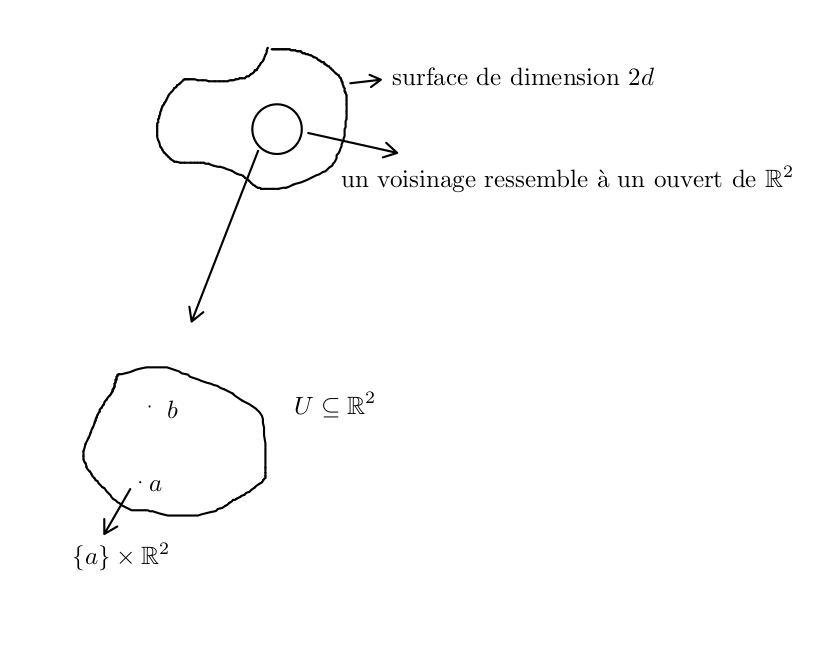
\includegraphics[scale=0.3]{figures/motiv1.png}
  \caption{Dans ce cas, \(\mathbb{R}^2\) est tangent partout.}
  \label{}
\end{figure}

\begin{figure}[h!]
  \centering
  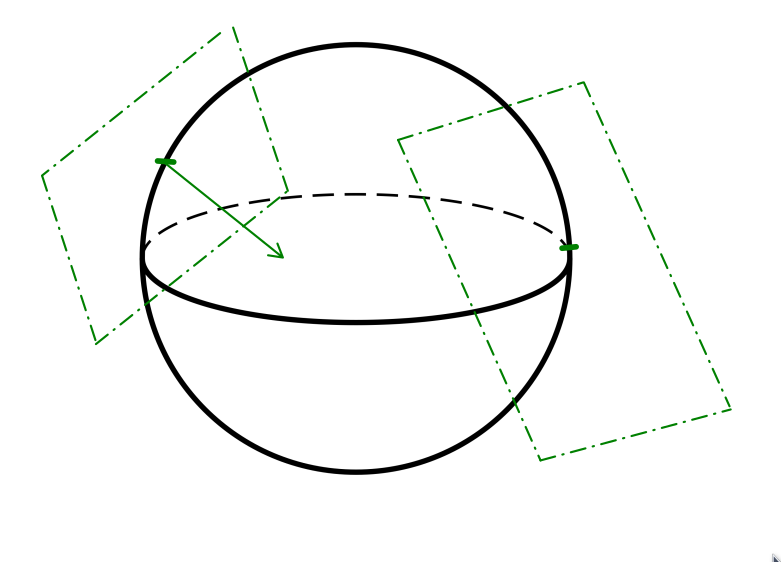
\includegraphics[scale=0.2]{figures/motiv2.png}
  \caption{Dans ce cas, chaque vecteur tangent est à l'intérieur et chaque plan tangent est différent.}
  \label{}
\end{figure}

\begin{definition}
  Soit \(U \subseteq \mathbb{R}^2\) un ouvert. Pour tout \(a \in U\), l'espace tangent

  \[T_a U \stackrel{\text{déf}}{=} \{ a \} \times \mathbb{R}^{n},\]

  et est muni d'un espace vectoriel de manière suivante :

  \[\forall u,v \in \mathbb{R}^n, \underbrace{(a,u)}_{\in T_a U} + (a,v) = (a, u+v),\]

  \[\forall r \in \mathbb{R}, \forall v \in \mathbb{R}^n, r(a,u) = (a, ru).\]
\end{definition}

\(T_a U\) devient un espace vectoriel linéairement isomorphe à \(\mathbb{R}^n\). Géométriquement on peut penser à \(T_a U\) comme un vecteur de \(\mathbb{R}^n\) basé en un point \(a\).

\begin{figure}[h!]
  \centering
  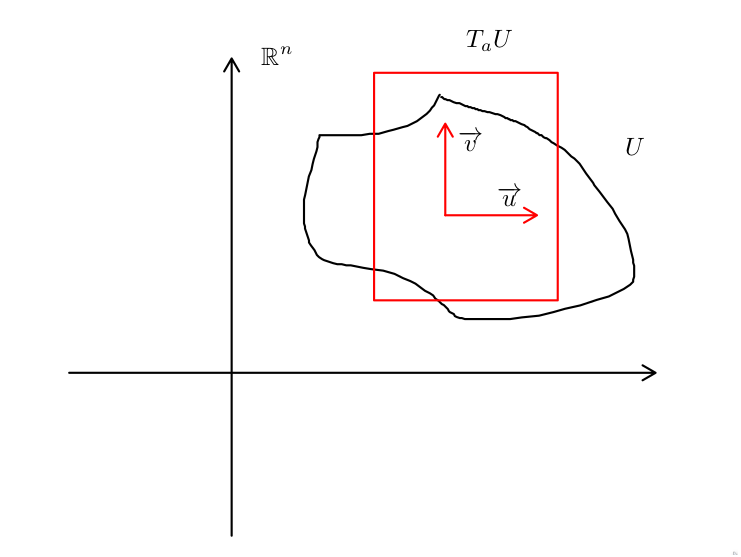
\includegraphics[scale=0.3]{figures/plan_tangent.png}
  \caption{Exemple d'un plan tangent à \(U\).}
  \label{}
\end{figure}

\subsection{Dérivation d'une fonction}

\begin{definition}
  Soit \(f : U \to \mathbb{R}^n\). Pour tout \(a \in U, Df(a) : \mathbb{R}^n \longrightarrow \mathbb{R}^m\). C'est une application linéaire.

  On va définir

  \[d_a f = df(a) : T_a U \longrightarrow \mathbb{R}^n,\]

  avec \[\underbrace{d f((a,\overrightarrow{v} ))}_{a \in U,\overrightarrow{v} \in \mathbb{R}^n  } = Df(a)(\overrightarrow{v}).\]

  Si \(a \neq b\), \(d_a f\) ne peut pas agir sur \(T_a U\) (formellement, ce n'est pas défini.

  On dit que \(d_a f\) est la dérivée de \(f\) au point \(a\).
\end{definition}

\begin{remark}[Personnelle]
  C'est la différentielle définie sur un espace tangent.
\end{remark}

\begin{remark}
  Si \(m=1\), \(d_a f \in \mathscr{L}(T_a U, \mathbb{R})\), c'est-à-dire que \(d_a f \in (T_a U) ^{*}\).
\end{remark}


\begin{remark}[Notation]
  \(T_a ^{*} U := (T_a U)^{*} \simeq \{ a \} \times (\mathbb{R}^n)^{*}\).
\end{remark}

\begin{definition}
  Le fibré tangent sur \(U\) est

  \[T U := \bigcup _{a \in U} \underset{(a,\overrightarrow{ v } ), \overrightarrow{ v } \in \mathbb{R}^n }{T_a U} \simeq U \times \mathbb{R}^n\]

  et le fibré cotangent est \[T ^{*} U := \bigcup _{a \in U} \underset{(a,f), f \in (\mathbb{R}^*)^{n}}{T_a ^{*} U} \simeq U \times (\mathbb{R}^{*})^{n}. \]
\end{definition}

Avec ce formalisme, la différentielle de \(f : U \longrightarrow \mathbb{R}^n\) est définie par \( df : U \longrightarrow T ^{*} U\) et \(\forall a \in U, d f(a) = d_a f \in T_a ^{*} U \subseteq T ^{*} U\).

\begin{remark}
  {\fontencoding{U}\fontfamily{futs}\selectfont\char 66\relax} Une condition nécessaire pour qu'une application \(\alpha : U \longrightarrow T ^{*} U\) soit une différentielle soit dans la forme \(\alpha = df\) est que pour tout \(a \in U, \alpha(a) \in T ^{*} U\).
\end{remark}

Si on définit \(\pi : T_a ^{*} \longrightarrow U\) par \(\pi(a,f) = a\), cette condition nécessaire est équivalente que de dire que \(\pi \circ \alpha = \mathds{1}_{U}\).

\begin{exemple}[De différentielle]
  Projection sur le composant \(j\) :

  On a \(x ^{ j} : U \longrightarrow \mathbb{R}\) telle que

  \[x ^{j}(a_1, \dots, a_n) = a_j.\]

  \[d_a x ^{j}(a, \overrightarrow{v}) = D x ^{j}(a)(\overrightarrow{v}) = \left[\frac{\partial x ^{j} }{\partial x_1}, \dots, \frac{\partial x ^{j} }{\partial x_n}\right] \left[\begin{matrix}
    v_1 \\
    \vdots \\
    v_n
  \end{matrix}\right] = [0, \dots, 0, \underset{\text{en } j}{1},0, \dots, 0] \left[\begin{matrix}
    v_1 \\
    \vdots \\
    v_n
  \end{matrix}\right] = v_j.\]
\end{exemple}

On a \(d x ^{j} : U \longrightarrow T ^{*} U\). Pour tout \(a \in U\), \(d x ^{j}(a) \in T_a^{*}U\).

Donc \(d x ^{j}(a) = (a,f)\) où \(f \in (\mathbb{R}^n)^{*}\). Pour tout \(\overrightarrow{ v }  \in \mathbb{R}^n\), \(f(\overrightarrow{v}) = v_j\). Pour \(e_i \in \mathbb{R}^n, f(e_i) = \delta _{i}^{j}\), donc \(f = e_j\), l'élément de la base duale. On a alors

\[d x ^{j}(a)=(a, e ^{j}).\]

Donc \((d x ^{1}(a), \dots, d x ^{n}(a))\) est une base naturelle pour \(T_a^{*} U\). La base duale de cette base dans \(T_a U \simeq (T_a ^{*}U)^{*}\) est décrite par la notation suivante :

\[\left(\frac{\partial  }{\partial x ^{1}}(a), \dots, \frac{\partial  }{\partial x ^{n}}(a)\right) = ((a,e_1), \dots, (a,e_n)).\]

On a \(\displaystyle\frac{\partial  }{\partial x ^{j}}(a) = (a, e_j), (d x ^{j}(a))\displaystyle\left(\frac{\partial  }{\partial x ^{i}}\right) = \delta^{j}_{i}\).

On suppose que \(E= T_a U\). On peut construire \(\Omega ^{k}(T_a U), \Omega _{l}(T_a U) = \Omega _{l}(T_a ^{*} U), \Omega _{l}^{k}(T_a U)\) qui sont des \((l,k)\)-tenseurs sur \(T_a U\).

On peut aussi définir \(\Lambda ^{k}(T_a U)\) (tenseurs extérieurs covariants), \(\Lambda _{l}(T_a U) = \Lambda ^{l}(T_a ^{*}U)\) (tenseurs extérieurs contravariants), \(\Lambda ^{k}_{l}(T_a U)\).

\begin{definition}
  On définit \[(T ^{k}_{l})_a U = \Omega ^{k}_{l}(T_a U)\] et \[(\Lambda _{l}^{k})_a U  \stackrel{\text{déf}}{=} (\Lambda ^{k}_{l})(T_a U).\]
\end{definition}

Si \(k=l=0\), on ne va pas les écrire.

\begin{definition}
  On peut alors définir les fibrés tensoriels et tensoriels extérieurs par :

  \[T ^{k}_{l} U := \bigcup _{a \in U} (T ^{k}_{l})_a U \text{  et } \Lambda ^{k}_{l} := \bigcup _{a \in U} (\Lambda ^{k}_{l})_a U.\]
\end{definition}



Très souvent on va avoir affaire aux fibrés où soit \(k\) soit \(l\) vaut 0. Par exemple,

\begin{gather*}
  \Lambda ^{k} U = \bigcup _{a \in U} \Lambda_a^{k} U = \bigcup _{a \in U} \Lambda ^{k}(T_a U), \\
  T ^{k} U = \bigcup _{a \in U} T_a ^{k} U = \bigcup _{a \in U} \Omega ^{k}(T_a U).
\end{gather*}

Si \(\alpha \in T _{l}^{k} U\), alors il existe \(a \in U\) tel que \(\alpha \in (T_l ^{k})_a U = \Omega ^{k}_{l}(T_a U)\). Donc \(\alpha\) est une application \((k+l)\)-linéaire sur \(\underbrace{T_1 U \times \dots \times T_a U}_{k \text{ fois}} \times \underbrace{(T_a U)^{*} \times \dots \times (T_a U)^{*}}_{l \text{ fois}}\).

Mais une telle application peut être identifiée par une application \((k+l)\)-linéaire sur \[\underbrace{\mathbb{R}^n \times \dots \mathbb{R}^n}_{k \text{ fois}} \times \underbrace{(\mathbb{R}^n)^{*} \times \dots \times (\mathbb{R}^n)^{*}}_{l \text{ fois}}\] avec les isomorphismes \(T_a U \simeq \mathbb{R}^n\), \(T_a ^{*} U \simeq (\mathbb{R}^n)^{*}\).

Donc \(\Omega ^{k}_{l}(T_a U) \simeq \{ a \} \times \Omega ^{k}_{l}(\mathbb{R}^n)\) et on a une projection bien définie sur la première composante

\[\tau _{l}^{k} : \Omega _{l}^{k}(T_a U) \longrightarrow U, \tau _{l}^{k}(a, \tilde{\alpha}) = a.\]

Donc si \(\alpha \in T _{l}^{k}U \), on a \(\tau _{l}^{k}(\alpha)\) est le point \(a \in U\) pour lequel \(\alpha \in (T _{l}^{k})_a U\).

\begin{definition}
  Un champ tensoriel sur \( U \subseteq \mathbb{R}^n\) est une application

  \[\alpha : U \longrightarrow T _{l}^{k} U\]

  telle que \[\tau _{l}^{k} \circ \alpha = \mathds{1}_{U}, \text{ avec } \tau _{l}^{k}(\alpha(a))=a.\]
\end{definition}

\begin{figure}[h!]
  \centering
  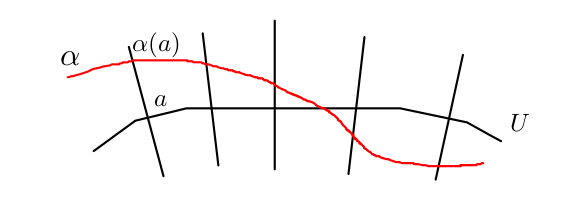
\includegraphics[scale=0.3]{figures/ch_tensoriel.png}
  \caption{Exemple d'un champ tensoriel}
  \label{}
\end{figure}

\(\alpha\) est aussi appelée parfois une section du fibré tensoriel \(T ^{k}_{l} U\).

Si \(\alpha\) est un champ tensoriel, pour tout \(a \in U\), \(\alpha(a) \in \Omega _{l}^{k}(T_a U)\).

L'ensemble \((e ^{i_1} \otimes \dots \otimes e ^{i_k} \otimes e _{j_1} \otimes \dots \otimes e _{j_k})\) est une base de \(\Omega _{l}^{k}(\mathbb{R}^n)\) où \(1 \leq i_1, \dots, i_k, j_1, \dots, j_l \leq  n\). Maintenant la base de \(\Omega^{k}_{l}(T_a U)\) devient

\[d x ^{i_1}(a) \otimes \dots \otimes d x ^{i_k}(a) \otimes \frac{\partial }{\partial d x ^{j_1} }(a) \otimes \dots \otimes \frac{\partial  }{\partial x ^{j_l}}(a).\]

Donc pour tout \(a \in U\), il existe des coefficients \(a _{i_1 \dots i_k}^{j_1 \dots j_l}(a) \in \mathbb{R}\) tels que :

\[\alpha(a) = \sum_{\substack{1 \leq  i_1, \dots, i_k \leq  n \\ 1 \leq j_1, \dots, j_l \leq  n}}^{} a ^{j_1 \dots j_l}_{i_1 \dots i_k} d x ^{i_1} \otimes \dots \otimes d x ^{i_k} \otimes \frac{\partial  }{\partial x ^{j_1}}(a) \otimes \dots \otimes \frac{\partial  }{\partial x ^{j_l}}(a).\]

\begin{figure}[h!]
  \centering
  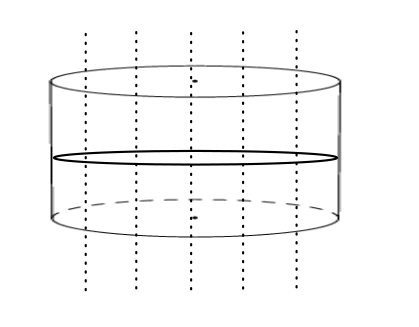
\includegraphics[scale=0.3]{figures/cylindre_tens.png}
  \caption{Cylindre \(S ^{1} \times \mathbb{R}^2\). On peut ``couper'' et considérer les cylindres \(S ^{1} \times [-1, 1]\).}
  \label{}
\end{figure}

\begin{figure}[h!]
  \centering
  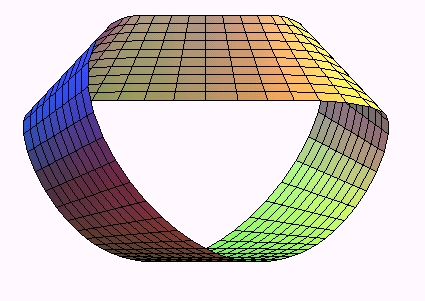
\includegraphics[scale=0.3]{figures/ruban_mobius.jpg}
  \caption{Le Ruban de Mobius n'est pas équivalent à \(S ^{1} \times [-1, 1]\)}
  \label{}
\end{figure}

Donc

\[\alpha = \sum_{1 \leq  i_1, \dots, i_k, j_1, \dots, j_l \leq  n} a _{i_1 \dots i_k}^{j_1 \dots j_l} d x ^{i_1} \otimes \dots \otimes d x ^{i_k} \otimes \frac{\partial  }{\partial x ^{j_1}} \otimes \dots \otimes \frac{\partial  }{\partial x ^{j_l}}\]

où \(a _{i_1 \dots i_k} ^{j_1 \dots j_l} : U \longrightarrow \mathbb{R}\) est une application.

\begin{definition}
  On dit que le champ vectoriel \(\alpha\) est de classe \(\mathcal{C}^r\) si \(\forall i_1, \dots, i_k, j_1, \dots, j_l\), le coefficient \[\alpha _{i_1 \dots i_k}^{j_1 \dots j_l} \in \mathcal{C}^r(U).\]
\end{definition}

Donc on peut parler de régularité de \(\alpha : U \longrightarrow \mathbb{R} ^{n+ n ^{k+l}}\) directement, mais dans ce cas là, la définition revient à la même.

\subsubsection{Exemple très important : la métrique riemanienne}

\begin{definition}
  Soit \(U \subseteq \mathbb{R}^n\) ouvert. Une métrique riemanienne sur \(U\) est un champ tensoriel 2-covariant (de type (0,2)) symétrique, positif-défini ur \(U\).
\end{definition}

Si \(g\) est une métrique riemanienne sur \(U\), \(g : U \longrightarrow T ^2 U\).

Pour tout \(x \in U, g(a) \in \Omega ^{2}(T_a U)\), avec \(\tau ^2 \circ g = \mathds{1}_{U}\).

\[\forall \overrightarrow{ u }, \overrightarrow{ v } \in T_a U, g(a)(\overrightarrow{ u }, \overrightarrow{ v }  ) = g(a)(\overrightarrow{ v }, \overrightarrow{ u }) \text{ (symétrie)}.\]

Donc cela revient à dire que \(g(a)\) est un produit scalaire sur \(T_a U\) (mais qui dépend de \(a\)).

La métrique riemanienne est donc un champ tensoriel de type (0,2) tel que \(\forall a \in U\), \(g(a)\) est un produit scalaire sur \(T_a U\).

Donc \[g = \sum_{1 \leq  i_1, i_2 \leq n} g _{i_1 i_2} d x ^{i_1} \otimes d x ^{i_2} = \sum_{1 \leq i, j \leq n} g _{ij} d x ^{i} \otimes d x ^{j}.\]

\emph{Quelle est la condition sur les coefficients \(g _{ij}\) pour que \(g\) devienne une métrique riemanienne ?}

Pour tout \(x \in U\), on peut former la matrice \[G_a = [g _{ij}(a)]_{n \times n}.\]

\begin{prop}
  \(g(a)\) est une métrique riemanienne sur \(T_a U\) si et seulement si \(g(a)\) est un produit scalaire.
\end{prop}

\begin{lemma}
  \(g(a)\) est un produit scalaire sur \(T_a U\) si et seulement si \(G_a\) est une matrice symétrique définie positive.
\end{lemma}

\begin{proof}
  \begin{gather*}
    g(a)\left(\frac{\partial  }{\partial x ^{i'}}, \frac{\partial  }{\partial x ^{j'}}\right) = \sum_{1 \leq i, j \leq  n} g _{ij}(a) d x ^{i}(a) \otimes d x ^{j}(a) \left(\frac{\partial  }{\partial x ^{i'}}(a), \frac{\partial  }{\partial d x ^{j'}}  \right) \\
    = \sum_{1 \leq i,j \leq n} g _{ij}(a) d ^{i}(a)\left(\frac{\partial  }{\partial x ^{i}}(a) \right) d x ^{j}(a) \left(\frac{\partial  }{\partial x ^{j}}(a) \right)  = \sum_{1 \leq i, j \leq n} g _{ij}(a) \delta _{i'}^{i} \delta _{j'}^{j} = g _{i'j'}(a).
  \end{gather*}

  Donc \(\forall i, j\),

  \[g _{i'j'}(a) = g(a) \left(\frac{\partial  }{\partial x ^{i'}(a)},\frac{\partial  }{\partial x ^{j'}}(a) \right) = g(a)\left(\frac{\partial  }{\partial x ^{j'}(a)},\frac{\partial  }{\partial x ^{i'}}(a) \right) = g _{j'i'}(a), \]

  ce qui implique que \(^{t}G_a = G_a\), donc \(G_a\) est symétrique.
\end{proof}

Supposons que \(g(a)\) est défini positif.

\begin{gather*}
  g(a)(\overrightarrow{v}) = \sum_{i,j}^{} d x ^{i}(a) \otimes d x ^{j}(a)(\overrightarrow{v}, \overrightarrow{v}),
\end{gather*}

avec

\begin{gather*}
  \overrightarrow{v} = \sum_{j=1}^{n} v ^{j} \frac{\partial  }{\partial x ^{j}} = \sum_{i,j}^{} g _{i,j}(a) d x^{i}(a) \otimes d x^{j}(a) \left(\sum_{i'}^{} \frac{\partial  }{\partial x ^{i'}}(a), \sum_{j'}^{} v ^{j'} \frac{\partial  }{\partial x ^{j'}}(a)\right) \\
  = \sum_{i,j} \sum_{i',j'} g _{ij}(a) v ^{i'} v ^{j'} d x^{i}(a) \left(\frac{\partial  }{\partial x ^{i'}}(a) d x^{j}(a) \frac{\partial  }{\partial x ^{j'}}(a) \right)=\sum_{\substack{i,j \\ i' = i \\ j=j'}} g _{ij}(a) v ^{i} v ^{j} \\
  = [v ^{1} \ \dots \ v ^{n}] [G_a] \left[\begin{matrix}
    v ^{1} \\
    \vdots \\
    v ^{n}
  \end{matrix}\right] = \tilde{\overrightarrow{v}} \cdot G_a \tilde{\overrightarrow{v}}.
\end{gather*}

%\begin{gather*}
%  \overrightarrow{v} = \sum_{j=1}^{n} v ^{j} \frac{\partial  }{\partial x ^{j}} = \sum_{i,j} g _{i,j} (a) d x ^{i}(a) \otimes d x ^{j}(a) \left(\sum_{i'} \frac{\partial  }{\partial x ^{i'}}(a), \sum_{j'} v ^{j'} \frac{\partial  }{\partial x ^{j'}}(a)\right) \\
%  = \sum_{i,j} \sum_{i',j'} g _{ij}(a)v ^{i'} v ^{j'} d x ^{i}(a) \left(\frac{\partial  }{\partial x ^{i'}}(a)\right)  d x ^{j}(a) \frac{\partial  }{\partial x ^{j'}}(a) \right)  = \sum_{\substack{i,j\\i' = i\\j'=j}} g _{ij}(a) v ^{i} v ^{j} \\
%  = [ v ^{1} \dots v ^{n}] [G_a] \left[\begin{matrix}
%    v ^{1} \\
%    \vdots \\
%    v ^{n}
%  \end{matrix}\right] = \tilde{\overrightarrow{v}} \cdot G_a \tilde{\overrightarrow{v}}.
%\end{gather*}

Donc \(\tilde{\overrightarrow{v}} G_a \tilde{\overrightarrow{v}} \geq 0\) pour tout \(\overrightarrow{v} \in \mathbb{R}^n\) et \(\tilde{\overrightarrow{v}} \cdot G_a \tilde{\overrightarrow{v}} = 0 \iff \tilde{\overrightarrow{v}} = 0\), ce qui implique que \(G_a\) est défini positif.

Le sens réciproque est démontré par les mêmes calculs.

\paragraph{Commentaires}

\begin{enumerate}
  \item Si \(G \in r ^{n+n}\) est symétrique et défini positif, alors \(\forall \overrightarrow{u}, \overrightarrow{v} \in \mathbb{R}^n\),

  \begin{gather*}
    \langle \overrightarrow{u} \mid \overrightarrow{v} \rangle _{G} := \overrightarrow{u} \cdot G \overrightarrow{v} = ^{t} \overrightarrow{u} G \overrightarrow{v} = \langle \overrightarrow{u} \mid G \mid \overrightarrow{v} \rangle
  \end{gather*}

  est un produit scalaire.

  \item Si \(\langle \overrightarrow{u} \mid \overrightarrow{v} \rangle \) est un produit scalaire sur \(\mathbb{R}^n\), alors il existe une matrice \(G\) dans \(\mathbb{R} ^{n+n}\) symétrique, définie positive telle que

  \[\langle \overrightarrow{u},\overrightarrow{v} \rangle _{*} = \langle \overrightarrow{u} \mid G \mid \overrightarrow{v} \rangle,  \]

  avec \(G = [g _{ij}] _{i,j}\) et \(g _{ij} = \langle e _{i} \mid e _{j} \rangle _{*} \).
\end{enumerate}

Donc pour la métrique riemanienne,

\[g = \sum_{i,j} g _{ij} d x^{i} \otimes d x^{j}, \]

avec \[g _{ij}(a) = g \left(\frac{\partial  }{\partial x ^{i}}(a), \frac{\partial  }{\partial x ^{j}}(a)\right).\]

Pour tout \(i\), \(\frac{\partial  }{\partial x ^{i}}(a) = (a, e_i) \in T_a U\) et

\[\left(\frac{\partial  }{\partial x ^{1}}(a), \dots, \frac{\partial  }{\partial x ^{n}}(a)\right)\]

est une base de \(T_a U = \{ a \} \times \mathbb{R}^n, a \in U\).

\(g : U \longrightarrow T ^2 U, \tau ^2 \circ g (a) = a, \forall a \in U\) si et seulement si \(\forall a \in U, g(a) \in T_a U\).

La métrique \(g\) est de classe \(\mathcal{C}^r\) si et seulement si \(\forall i, j, g _{ij} : U \longrightarrow \mathbb{R}\) est de classe \(\mathcal{C}^r\) (par définition).

\begin{exemple}[La métrique euclidienne]
  \[g = \sum_{i=1}^{n} d x^{i} \otimes d x^{i}\]

  et \[\forall a \in U, G_a = I _{n+n} \in \mathbb{R} ^{n+n}.\]

  Supposons \(\gamma : [a,b] \longrightarrow U\) différentiable, avec \([a,b] \subset \mathbb{R}\).

  On a, pour \(\gamma(t) = (x ^{1}(t), \dots, x ^{n}(t) )\), \((\gamma)'(t) = (x ^{1})'(t), \dots, (x ^{n})'(t)\),

  \begin{gather*}
    L(\gamma) = \int_{a}^{b} \left\Vert \gamma'(t) \right\Vert  dt = \int_{a}^{b}(\gamma'(t) \cdot I _{n+n} \gamma'(t)) ^{\frac{1}{2}}dt = \int_{a}^{b}\langle \gamma'(t) \mid \gamma'(t) \rangle _{I _{n+n}}^{\frac{1}{2}}dt
  \end{gather*}
\end{exemple}


  On va définir, pour \(\gamma : (a,b) \longrightarrow U\),

  \[T \gamma : \underbrace{T _{(a,b)}}_{(t,\overrightarrow{v}), \overrightarrow{v} \in \mathbb{R}}  \longrightarrow \underbrace{T U}_{(c,\overrightarrow{w}), c \in U, \overrightarrow{w} \in \mathbb{R}^n}.\]

  \(g(\gamma(t))\) est un produit scalaire sur \(T _{\gamma(t)} U\) et

  \[T \gamma(t,\overrightarrow{v}) = (\gamma(t), \overrightarrow{v}\gamma'(t)).\]

  Choisissons \(\{ 1 \}\) comme base de \(\mathbb{R}\). Alors

  \begin{enumerate}
    \item \[T \gamma _{\mid T _{t}(a,b)} : T _{t (a,b)} \longrightarrow T _{\gamma(t)} U.\]

    \item \(T \gamma (t,1) = (\gamma(t), \gamma'(t))\), avec \((t, 1)\) élément de base pour \(T _{t (a,b)}\).
  \end{enumerate}

  On définit alors

  \[L _{g}(\gamma) := \int_{a}^{b}g(\gamma(t))(T \gamma(t,1),T \gamma (t,1))^{\frac{1}{2}} dt. \]

Si \(g = \sum_{}^{} g _{ij} d x^{i} \otimes d x^{j}\) et \(G_c = [g _{ij}(c)], \forall c \in U\), on obtient

\[L _{g}(\gamma) = \int_{a}^{b} \langle \gamma'(t) \mid G _{\gamma(t)} \mid \gamma'(t) \rangle ^{\frac{1}{2}}dt.\]

\begin{remark}
  Si \(c, d \in U, c \neq d, \forall \gamma : [a,b] \longrightarrow U\) tel que \(\gamma(a)=c, \gamma(b)=d\) différentiable sur \((a,b)\), \(L_g(\gamma) \bg 0\).
\end{remark}

\begin{exo}
  Si \(\gamma'(t) = 0\), alors \( \gamma(t) \equiv \text{constant} \implies c=d \text{ impossible}\). Il exsite \(t_0 \in (a,b)\) tel que \(\gamma'(t_0) \neq 0 \implies \langle \gamma'(t_0) \mid G _{\gamma(t_0)} \mid \gamma'(t_0) \rangle  \bg 0\). Utiliser la continuité des acteurs pour conclure.
\end{exo}

\begin{definition}[Rappel : distance, espace métrique]

\end{definition}

\[\forall x, y \in U, d _{g}(x,y) = \inf \{ L _{g}(\gamma), \gamma : [a,b] \longrightarrow U, \gamma \text{ différentiable sur } [a,b], \gamma(a) = x, \gamma(b)=b\}.\]

\begin{thm}
  Si \( U \subseteq \mathbb{R}^n\) connexe par arcs et \(g\) est une métrique riemanienne continue sur \(U\), alors

  \[d_g : U \times U \longrightarrow \mathbb{R}\]

  est une distance sur \(U\) et \((U, d_g)\) devient un espace métrique.
\end{thm}

\begin{remark}[Point technique]
  Si \(U\) est connexe par arcs, \(\forall x, y \in U, \exists \gamma \in \mathcal{C}^0([0, 1], U)\), avec \(\gamma(0) = x, \gamma(1) = y\), alors (analyse réelle, on utilise le fait que \(U\) est ouvert) il existe \(\gamma \in \mathcal{C}^1([0,1], U)\) avec \(\gamma(0)=x, \gamma(1)=y\).
\end{remark}

Donc il existe un élément de \(\{ \gamma \in \mathcal{C}^1([a,b], U) \mid \gamma(a) = x, \gamma(b) = y\}\), avec \(a = 0, b=1\). Comme \(\gamma \in \mathcal{C}^1([a,b])\), \(\left\lvert \gamma'(t)\right\rvert\) est continue sur \([a,b]\) implique que il existe \(M \bg 0 \) tel que \( \forall t \in [a,b], \left\Vert \gamma'(t) \right\Vert \leq M\) et \(G _{\gamma(t)} :  [a,b] \longrightarrow \mathbb{R}^{n+n}\) est aussi continue.

Cela implique que \( t \longmapsto \langle \gamma'(t) \mid G _{\gamma(t)} \mid \gamma'(t)\rangle\) est continue sur \([a,b]\), ce qui implique que il existe \(\tilde{M}\) tel que

\[\forall t \in [a,b], \langle \gamma'(t) \mid G _{\gamma(t)} \mid \gamma'(t) \rangle ^{\frac{1}{2}} \leq \tilde{M},\]

ce qui implique que

\[L _{g}(\gamma) = \int_{a}^{b}\langle \gamma'(t)\mid G _{\gamma(t)} \mid \gamma'(t) \rangle \leq \tilde{M}(b-a) \less + \infty, \]

donc \(d_g(x,y)\) ne peut être \(+\infty\), \(d_g(x,y) \in \mathbb{R} _{+}\). Donc \(d_g : U \times U \longrightarrow \mathbb{R}\) est justifié.

\begin{remark}

  \

  \begin{enumerate}
    \item Si \(U\) n'est pas connexe, il faut faire attention que le chemin droit de \(x\) à \(y\) peut sortir de \(U\) et n'est pas éligible pour évaluer \(L _{g}(\gamma)\).
    \item Même si \(U\) est connexe, il n'y a pas de raison que le chemin sur le segment droit joignant \(x\) à \(y\) est le chemin le plus court :

    \[\gamma(t) = x + t(y-x), \gamma : [0, 1] \longrightarrow U.\]

    Il peut arriver que \[d_g(x,y) \less L_g(\gamma) = \int_{0}^{1} \langle y-x \mid G _{\gamma(t)} \mid y-x \rangle dt. \]

    \item Pas toutes les métriques \(d\) des espaces métriques \((X,d)\) où \(X\) est un ouvert de \(\mathbb{R}^n\) sont  les distances \(d_g\) pour la métrique riemanienne. Par exemple, \(d(x,y) = 1 \text{ si } x=y \text{ et } d(x,y) =0\) sinon ne peut pas dériver de la métrique riemanienne.

    \item On peut remplacer les chemins \(\gamma\) par les chemins \(\mathcal{C}^1\) par morceaux ou bien par les chemins polygonaux.
  \end{enumerate}
\end{remark}

\begin{definition}
  \((U,g)\) où \(g\) est une métrique riemanienne et \(U \subseteq \mathbb{R}^n\) est un exemple d'une variété riemanienne.
\end{definition}

\begin{definition}
  Supposons que \((x, \overrightarrow{v}), (x, \overrightarrow{v}) \in T_x U\) pour \(x \in U\). Alors l'angle entre ces deux vecteurs est défini par

  \[\sphericalangle (x,\overrightarrow{u}), (x, \overrightarrow{v}) = \cos ^{-1}\left(\frac{g(x)((x,\overrightarrow{u}), (x,\overrightarrow{v}))}{\left\Vert (x,\overrightarrow{u}) \right\Vert _{g} \left\Vert (x,\overrightarrow{v}) \right\Vert  }\right).\]
\end{definition}

\begin{remark}[Rappel]
  Pour tout produit scalaire \(\langle \mid \rangle _{*}\), l'inégalité de Cauchy-Schwarz est valide, c'est-à-dire :

  \[\forall \overrightarrow{u}, \overrightarrow{v} \in E, \left\lvert \langle \overrightarrow{u} \mid \overrightarrow{v} \rangle  \right\rvert \leq  \langle \overrightarrow{u} \mid \overrightarrow{u} \rangle _{*}^{\frac{1}{2}} \langle \overrightarrow{v} \mid \overrightarrow{v} \rangle _{*} ^{\frac{1}{2}}.  \]

  Donc pour tout \(\overrightarrow{u}, \overrightarrow{v} \in T_x U, \left\lvert g(a)(\overrightarrow{u}, \overrightarrow{v}) \right\rvert \leq  \left\Vert \overrightarrow{u} \right\Vert _{g} \left\Vert \overrightarrow{v} \right\Vert _{g}\).
\end{remark}

Avec la notation qu'on a eu sur la norme \( \left\Vert  \cdot \right\Vert _{g} \), on a, pour tout \(\gamma : [a,b] \longrightarrow \mathbb{R}\) différentiable,

\[L _{g}(\gamma) = \int_{a}^{b} \underbrace{\left\Vert T \gamma(t,1) \right\Vert _{g}}_{(\gamma(t), \gamma'(t))} dt.\]

\begin{exemple}[Demi-plan de Poincaré (exemple de variété riemanienne) de dimension 2 et de géométrie non-euclidienne]

  \[U = \{ (x,y) \in \mathbb{R}^2 \mid y \bg 0 \}.\]

  On définit une métrique riemanienne sur \(U\) par

  \[g = \sum_{i=1}^{2}  g _{ii} d x^{i} \otimes d x^{i}, g _{ij}(x,y) = \delta _{ij} \frac{1}{y ^2} G _{(x,y)} = \left[\begin{matrix}
    \frac{1}{y ^2} & 0 \\
    0 & \frac{1}{y ^2}
  \end{matrix}\right]. \]
\end{exemple}

\begin{definition}
  Si pour une métrique riemanienne \(g\) donnée sur \(U\), il existe une fonction \(h : U \longrightarrow \mathbb{R}\) telle que

  \[\forall a \in U, g(a) = h(a) I _{n \times n} = \left[\begin{matrix}
    h(a) & \dots & 0 \\
    \vdots & \ddots & \vdots \\
    0 & \dots & h(a)
  \end{matrix}\right].\]

  On dit que \(g\) est une métrique conformale.
\end{definition}

Donc la métrique

\[g(x,y) = \frac{1}{y ^2}(dx \otimes dx + d y \otimes d y)\]

est une métrique riemanienne.

La géométrie induite par \(g\) sur le demi-plan est la géométrie hyperbolique, connue aussi sous le nom de la géométrie de Lebachowski.

\begin{thm}
  Si \(g\) est une métrique conformale sur \(U\) et \(\overrightarrow{u}, \overrightarrow{v} \in T_a U\) pour \(a \in U\), alors

  \[\sphericalangle _{g} \overrightarrow{u}, \overrightarrow{v} = \sphericalangle \overrightarrow{u}, \overrightarrow{v}\]

  pour la métrique standart euclidienne.
\end{thm}

\begin{figure}[h!]
  \centering
  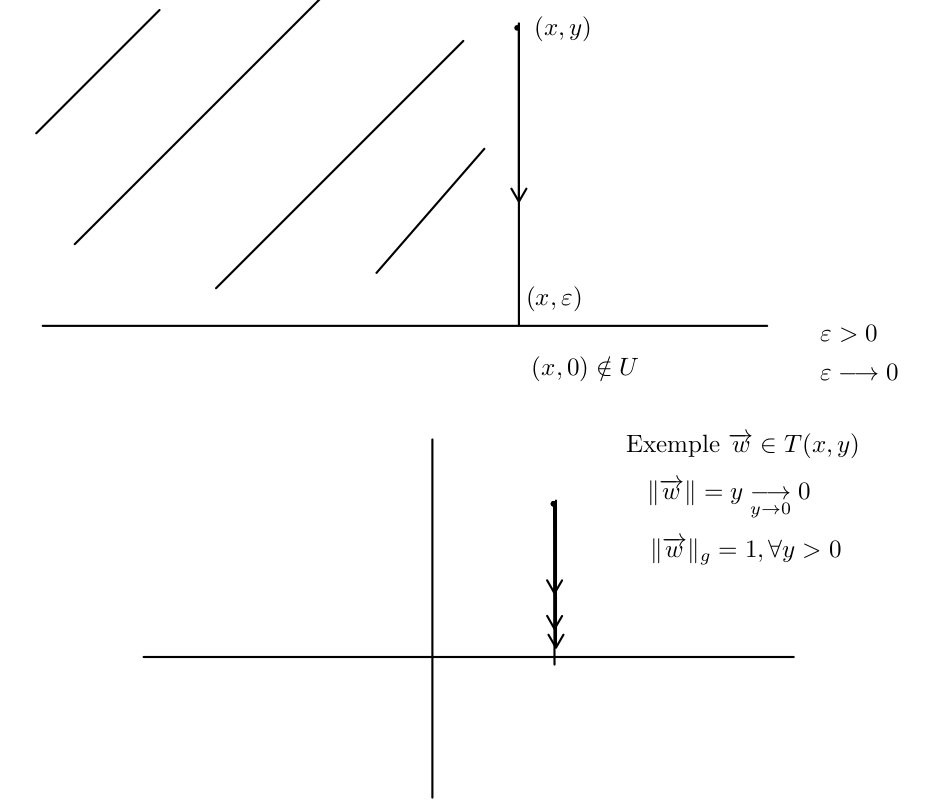
\includegraphics[scale=0.2]{figures/horizon1.png}
  \caption{}
  \label{horizon1}
\end{figure}

\begin{figure}[h!]
  \centering
  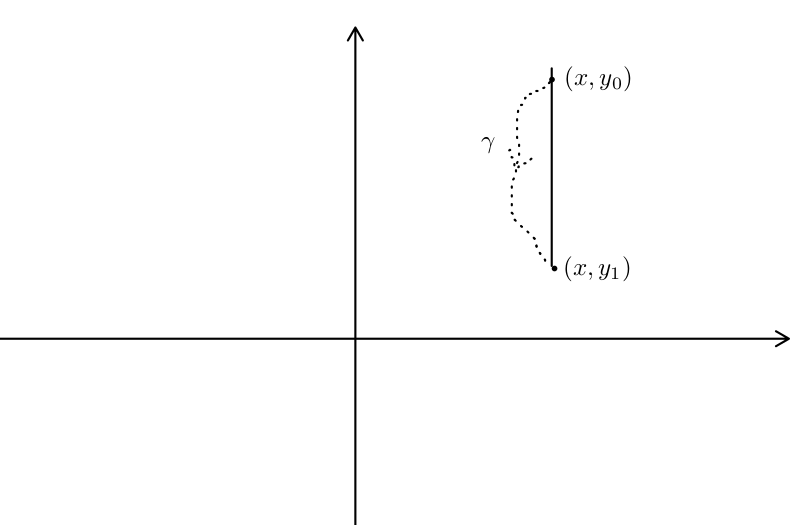
\includegraphics[scale=0.3]{figures/horizon2.png}
  \caption{}
  \label{horizon2}
\end{figure}

On a, pour le cas des figures \ref{horizon1} et \ref{horizon2}, le calcul suivant, pour \(\gamma(t) = (x(t), y(t))\) :

\begin{gather*}
  L_g(\gamma) = \int_{0}^{1}  \Vert \overbrace{y(t), \gamma'(t)}^{\in T _{\gamma}(t)} \Vert_g  dt = \int_{0}^{1} \frac{\left\Vert \gamma'(t) \right\Vert }{y}dt = \int_{0}^{1} \frac{\sqrt{(x')^2(t)+ (y')^2(t)}}{y(t)} dt.
\end{gather*}

On a \(\eta(t) = (x,y_0) + t((x,y_1)-(x,y_0)) = (x,y_0 + t(y_1 - y_0))\) et \(\eta'(t) = (0,y_1-y_0)\), ce qui donne \(\left\Vert \eta'(t) = \left\lvert y_1 - y_0 \right\rvert \right\Vert \). Donc

\begin{gather*}
  L_g(y) = \int_{0}^{1} \frac{\left\Vert \eta'(t) \right\Vert }{y_0 + t(y_1-y_0)}dt = \int_{0}^{1} \frac{\left\lvert y_1-y_0 \right\rvert}{y_0 + t(y_1-y_0)}dt.
\end{gather*}

Notez que si l'on choisit \(\tilde{\gamma}(t)=(x,y(t))\) en partant de \(\gamma(t) = (x(t),y(t))\), on a :

\begin{gather*}
  L_g(\tilde{\gamma}) = \int_{0}^{1} \frac{\left\Vert \tilde{\gamma}(t) \right\Vert }{y(t)}dt = \int_{0}^{1} \frac{\left\lvert y'(t) \right\rvert}{y(t)}dt \leq  \int_{0}^{1} \frac{\sqrt{(x')^2(t) + (y')^2(t)}}{y(t)}dt = L_g(\gamma).
\end{gather*}

\begin{figure}[h!]
  \centering
  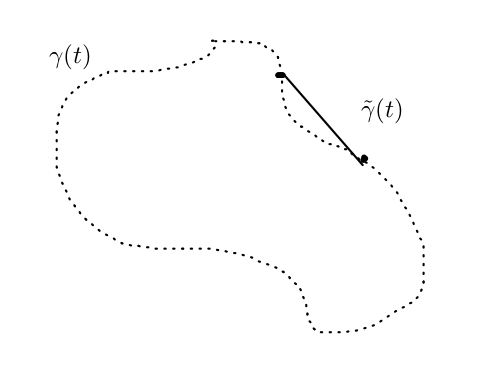
\includegraphics[scale=0.2]{figures/chemin-vert-court.png}
  \caption{Le chemin tout droit vertical est toujours le plus court}
  \label{chemin-vert-court}
\end{figure}

En conclusion, on a \(L_g(\tilde{\gamma}) \leq L_g(\gamma)\), ce qui signifie que le chemin tout droit vertical est toujours le plus court par rapport à tous les chemis qui joignent \((x,y_0)\) à \((x,y_1)\) comme illustré dans la figure \ref{chemin-vert-court}.

{\fontencoding{U}\fontfamily{futs}\selectfont\char 66\relax} On n'a pas dit que \(\eta\) donne la paramétrisation du chemin le plus court entre \((x,y_0)\) et \((x,y_1)\). C'est une question à discuter plus tard.

\begin{figure}[h!]
  \centering
  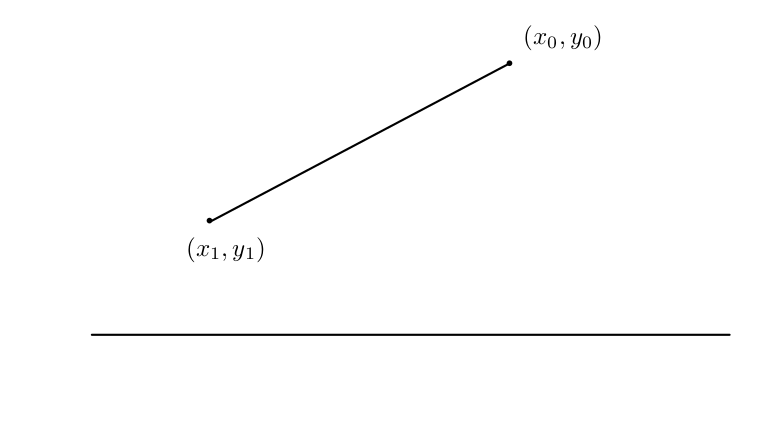
\includegraphics[scale=0.3]{figures/ligne-pas-tres-courte.png}
  \caption{La ligne droite n'est pas en général le chemin le plus court.}
  \label{}
\end{figure}

\

Si \(\overrightarrow{w} \in T _{(x,y)} U\) pour \((x,y) \in U\) quelconque, avec \(\overrightarrow{w} = (w_1, w_2)\), on a :

\[\left\Vert \overrightarrow{w} \right\Vert _{g} = (g(x,y)(\overrightarrow{w}, \overrightarrow{w})) ^{\frac{1}{2}} = \left(\frac{1}{y ^2} \left\Vert \overrightarrow{w}^2 \right\Vert \right) ^{\frac{1}{2}} = \frac{\left\Vert \overrightarrow{w} \right\Vert }{y}.\]

Si \(\gamma : [0, \infty) \longrightarrow U\), avec \(\gamma(0) = (x_0, y_0)\), \(\overrightarrow{w} =(0, -y) \in T _{(x,y)} U\), on cherche \(\gamma(t)\) tel que

\[\gamma'(t) =(0, -\gamma_2(t)),\]

avec \(\gamma(t) = (x(t), y(t)), \gamma_1(t) = x(t), \gamma_2(t) = y(t)\),

\[\begin{cases}
  x'(t) =0, x(t) \equiv x_0 \\
  y'(t)=0, y(t) \equiv y_0,
\end{cases}\]

alors \(y(t) = y_0 e^{-t} \). Donc \(\gamma(t) = (x_0, y_0 e^{-t})\) est le chemin partant de \((x_0, y_0)\) d'une manière verticale vers l'horizon \(y=0\) avec la vitesse hyperbolique constante.

On voit bien que \(\gamma(t) =(x_0, 0)\) donne \(t = +\infty\).

\

Il y a aussi le disque de Poincaré (Escher hyperbolic disc).

\begin{figure}[h!]
  \centering
  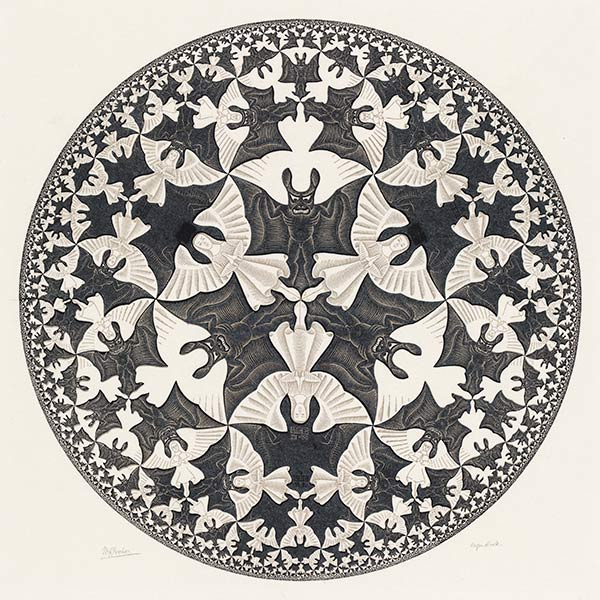
\includegraphics[scale=0.3]{figures/escher.jpg}
  \caption{Escher hyperbolic disc}
  \label{}
\end{figure}

Il faudra encore développer les techniques nécessaires pour pouvoir démontrer que les lignes droites par rapport à la métrique hyperbolique sur le demi-plan de Poincaré sont effectivement des demi-cercles centrés sur la ligne \(y=0\). Ces lignes droites sont appelées les géodésies de \((U,g)\) dans la géométrie différentielle.

Voici une première définition de la géodésie \ref{geodesie} (de manière rudimentaire plus géométrique que mécanique) :

\begin{definition}
  On dit que \(\gamma([a,b])\) est un segment géodésique dans \((U,g)\) si pour \(x = \gamma(a), y = \gamma(b), x, y \in U\),

  \[d _{g}(x,y) = L _{g}(\gamma).\]

  Une courbe \(\mathscr{C} \subseteq U\) est une géodésie de \((U,g)\) quand

  \[C = \bigcup _{i \in I} \mathscr{C}_i \]

  où chaque \(\mathscr{C}_i\) est un segment géodésique tel que \(\forall n \in \mathbb{Z}, C_n \cap C _{n+1}\) est un singleton.
\end{definition}

\begin{figure}[h!]
  \centering
  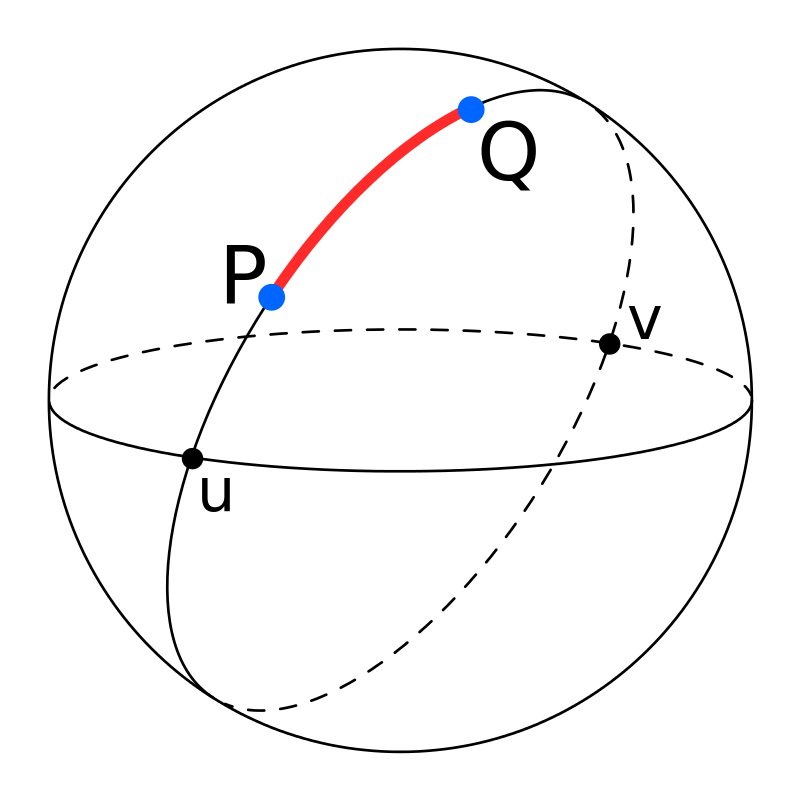
\includegraphics[scale=0.2]{figures/geodesie.png}
  \caption{Géodésie}
  \label{geodesie}
\end{figure}

\begin{remark}[Rappel]
  Soit \(\beta : E \times E \longrightarrow \mathbb{R}\) un produit scalaire sur un espace vectoriel \(E\). Soit \(f \in E ^{*}\), avec \(\operatorname{dim}(E) = n\). Alors il existe un vecteur \(\overrightarrow{v_f}\) unique tel que

  \[\forall \overrightarrow{w} \in E, f(\overrightarrow{w}) = \beta(\overrightarrow{v_f}, \overrightarrow{w}).\]
\end{remark}

\begin{exemple}
  Soit \(\beta\) donné par la matrice \(B \in \mathbb{R}^{n \times n}\) symétrique définie positive sur une base \((e_1, \dots, e_n)\) de \(E\). On a

  \[f(\overrightarrow{w}) = f \left(\sum_{i} w_i e_i \right) = \sum_{i} w_i f(e_i), \]

  avec \(\overrightarrow{v_f} = \sum_{j=1}^{n} x_j e_j \) (\((x_1, \dots, x_n)\) inconnues).

  \begin{gather*}
    \beta(\overrightarrow{v_f}, \overrightarrow{w}) = \langle \overrightarrow{v_f} \mid B \mid \overrightarrow{w} \rangle = \sum_{i,j=1}^{n} x_j b _{ij} w_i,
  \end{gather*}

  \(B = [b _{ij}] _{n \times n}\). On veut que \(\forall (w_i)_{i=1}^{n}\),

  \[\sum_{i} x_i f(e_i) = \sum_{i,j=1} x_j b _{ij} w_i\]

  si et seulement si

  \[\forall i, \sum_{j=1}^{n} b _{ij} x_j = f(e_i) \in \mathbb{R}.\]

  \begin{equation}\label{truc-long}
    [b _{ij}] \left[\begin{matrix}
      x_1 \\
      \vdots \\
      x_n
    \end{matrix}\right] = \left[\begin{matrix}
      f(e_1) \\
      \vdots \\
      f(e_n)
    \end{matrix}\right].
  \end{equation}

  \(f\) étant donné, comme \(\operatorname{det}(B) \neq 0\), il existe un unique \(x = (x_1, \dots, x_n) \in \mathbb{R}^n\) qui satisfait \ref{truc-long}, et donc

  \[\overrightarrow{v_f} = \sum_{i} x_i e_i \] est la réponse unique.
\end{exemple}

\begin{definition}[Rappel : gradient euclidien]
  Soit \(f : U \longrightarrow \mathbb{R} \text{ différentiable } , U \subseteq \mathbb{R}^n\) et

  \[\nabla f(a) = (\partial_1 f(a), \dots, \partial_n f(a)).\]
\end{definition}

\(Df(a) : \mathbb{R}^n \longrightarrow \mathbb{R}\) application linéaire de \((\mathbb{R}^n)^{*}\).

\[\forall \overrightarrow{v} \in \mathbb{R}^n, Df(a)(\overrightarrow{v}) = \langle Df(a), \overrightarrow{v}\rangle\]

avec la métrique euclidienne.

\

Soit \((U,g)\) une métrique riemanienne, \(U \subseteq \mathbb{R}^n\), \(f : U \longrightarrow \mathbb{R}\) une application partout différentiable \(df : U \longrightarrow T ^{*} U\),

\[\forall a \in U, d_a f \in T ^{*}_{a} U = (T_a U)^{*},\]

où \(g(a)\) est un produit scalaire sur \(T_a U\). On prend \(E = T_a U, d_a f \in E ^{*}, \beta = g(a)\).

Donc il y a un vecteur unique \(\nabla_g f(a) \in T_a U\) tel que

\[\forall \overrightarrow{w} \in T_a U, d_a f(\overrightarrow{w}) = g(a) (\nabla_g f(a), \overrightarrow{w}).\]

Si \(g = \sum_{i,j} g _{ij} d x^{i} \otimes d x^{j}\), \(\nabla_g f(a) \in T_a U\), on a déjà vu que pour la métrique euclidienne \(g = eu\),

\[\nabla _{eu}f(a) = \sum_{i=1}^{n} \frac{\partial f }{\partial x ^{i}}(a) \frac{\partial  }{\partial x ^{i}}.\]

On peut aussi écrire

\[\nabla_g f(a) = \sum_{i=1}^{n}(?)_i \frac{\partial  }{\partial x ^{i}}(a).\]

Si \(\nabla _{g}f(a) = \sum_{i=1}^{n}c_i \frac{\partial  }{\partial x_i}(a)\), on écrit

\[\nabla _{g} f(a) = \mid \nabla_g f(a)\rangle = \left[\begin{matrix}
  c_1 \\
  \vdots \\
  c_n
\end{matrix}\right] = ?\]

Pour tout \(i\), on a \(d_a f\left(\frac{\partial  }{\partial x ^{i}}(a) \right) = g(a) (\nabla _{g}f(a), \frac{\partial  }{\partial x ^{i}}(a))\). Cela implique que

\begin{gather*}
  \forall i \in \{1, \dots, n \}, G_a = [g _{ij}], g(a) \left(\nabla_g f(a), \frac{\partial  }{\partial x ^{i}}(a)  \right) = \left\langle e_i \mid G_a \mid \nabla_g f(a) \right\rangle \partial_i f(a)
\end{gather*}

si et seulement si \[G_a \mid \nabla _{g}f(a) \rangle  = \left[\begin{matrix}
  \partial_1 f(a) \\
  \vdots \\
  \partial_n f(a)
\end{matrix}\right] \implies \left[\begin{matrix}
  c_1 \\
  \vdots \\
  c_n
\end{matrix}\right] = \mid \nabla_g f(a) \rangle = G_a ^{-1} \left[\begin{matrix}
  \partial_1 f(a) \\
  \vdots \\
  \partial_n f(a)
\end{matrix}\right].\]

Donc \(\mid \nabla _{g}f(a)\rangle = G_a ^{-1} \mid \nabla f(a)\rangle\).

\(G ^{-1}(a)\) est souvent représentée par une matrice \(g ^{ij}(a)\).  On a

\begin{gather*}
  \left(\sum_{k=1}^{n} g _{ik}(a)g ^{kj}(a) = \delta _{i}^{i} \right), \sum_{k=1}^{n} g ^{ik}g _{kj} = \delta _{j}^{i}
\end{gather*}

et

\begin{gather*}
  \left[\begin{matrix}
    c_1 \\
    \vdots \\
    c_n
  \end{matrix}\right] = [g ^{ij}(a)] \begin{bmatrix}
    \partial_1 f(a) \\
    \vdots \\
    \partial_n f(a)
\end{bmatrix},
\end{gather*}

donc \(\forall i\), \(\displaystyle \sum_{j=1}^{n} g ^{ij}(a) \partial_j f(a)\).

\begin{remark}
  \(\underbrace{d_a}_{\in T_a ^{*}U} = \displaystyle \sum_{i=1}^{n} \partial_i f(a) \underbrace{d x^{i}(a)}_{(a, e ^{ij})}\) (si \(\alpha = \displaystyle \sum a_i e ^{i}, a_i = \alpha(e_i)\) et \(d_a f(e_i) = \partial_i f(a)\)).

  Donc \(d_a f \in (T_a U)^{*} = \Omega ^{1}(T_a U)\), c'est un tenseur covariant d'ordre 1.
\end{remark}

Les coefficients sont indexés en base \(\partial_i f(a)\). La base indexée en haut est \(d x^{i}(a)\). On remarque que \(\nabla_gf(a) \in T_a U = \Omega_1(T_a U)\), c'est donc un tenseur contravariant d'ordre 1. Donc

\[\nabla_g f(a) = \sum_{i=1}^{n} c ^{j} \frac{\partial  }{\partial x ^{i}}(a).\]

On a pour tout \(i\),

\[c ^{i} = \sum_{j=1}^{n} g ^{ij}(a) \partial_j f(a).\]

On écrit

\[\underset{\text{dans } \Omega_1(T_a U)}{\nabla_g f(a)} = g _{\sharp}(\underset{\text{dans } \Omega ^{1}(T_a U)}{T_a U}).\]

Plus généralement, si \(\alpha : U \longrightarrow T_l ^{k} U\) est un champ tensoriel, i. e.

\[\alpha = \sum_{\substack{i_1, \dots, i _{k}\\ j_1, \dots, j_k}} a ^{j_1 \dots j_l}_{i_1 \dots i_k} d x^{i_1} \otimes \dots \otimes d x^{i_k} \otimes \frac{\partial  }{\partial x ^{j_1}} \otimes \dots \otimes \frac{\partial  }{\partial x ^{j_l}}\]

et \(g\) est une métrique riemanienne pour \(k \geq 1\), on peut créer un champ tensoriel dans \(T ^{k-1}_{l+1}\) de trace \(g\) que l'on notera \(g _{\sharp}\alpha : U \longrightarrow T ^{k-1}_{l+1} U\) et il vaudra :

\[g _{\sharp} \alpha= \sum_{\substack{1 \leq i_1 \dots i _{k-1} \leq n\\ 1 \leq j_1 \dots j _{l+1} \leq  n}} b _{i_1 \dots i _{k-1}}^{j_1 \dots j _{l+1}} d x^{i_1} \otimes \dots d x^{i _{k-1}} \otimes \frac{\partial  }{\partial x ^{j_1}} \otimes \dots \otimes \frac{\partial  }{\partial x ^{j _{l+1}}}.\]

Pour tous les choix, on a \(b _{i_1 \dots i _{k-1}}^{j_1 \dots j _{l+1}} = \displaystyle g ^{j _{l+1}i} a ^{j_1 \dots j_l}_{i_1 \dots i _{k-1}}i\).

\begin{exemple}[Tenseurs de courbure de Riemann]
  Parfois il est écrit comme \(R _{jkl}^{i}\) de type (1,3) ou comme \(R _{ijkl}\) de type (0,4).

  En fait \(R _{jkl}^{i} = \displaystyle\sum_{s=1}^{n} g ^{is} R _{sjkl} ; R _{ijkl} = \displaystyle\sum_{s=1}^{n} g _{is} R ^{s}_{jkl}\).

  \(d f(a) \in T_a ^{*}U\) ne dépend pas de \(g\) et \(\nabla_g f(a) \in T_a U\). Alors

  \begin{gather*}
    G_a \mid \nabla_g f(a)  \rangle = \mid \nabla f(a) \rangle \ ; \ \underbrace{\partial_i f(a)}_{\text{les coefs de } d f(a)} = \sum_{s=1}^{n} g _{is} C ^{s},
  \end{gather*}



  où \(\nabla_g f(a) = \displaystyle \begin{bmatrix}
    c_1 \\
    \vdots \\
    c_n
  \end{bmatrix}.\)

\end{exemple}

\subsection{Champ de vecteurs}\marginnote{19-10-2023}

\begin{definition}
  Un champ de vecteurs est une application \(X : U \longrightarrow T U\) telle que

  \[\forall a \in U, \tau_1 \circ X(a) = a \ (\tau_1 \circ X = id),\]

  c'est-à-dire \(X\) est un champ de tenseur 1-contravariant sur \(U\). En équivalence, \(X\) est une section de fibré tangent \(T U\).
\end{definition}

\(X\) est un champ de tenseurs de type (1,0) et

\[X  = \sum_{i=1}^{n} X ^{i} \frac{\partial  }{\partial x ^{i}}.\]

On a \(\forall a \in U\),

\[X(a) = \sum_{i=1}^{n} X ^{i}(a) \underbrace{\frac{\partial  }{\partial x ^{i}} }_{(a,e_i)}.\]

Pour tout \(i\), \(X : U \longrightarrow \mathbb{R}\) et on a \(X \in C ^{*}\) si et seulement si pour tout \(i\), \(X ^{i} \in C ^{*}\).

\begin{exemple}
  Soit \(I \subseteq \mathbb{R}\) un intervalle ouvert, par exemple \(I = (a,b)\). Soit \(\gamma : I \longrightarrow U\) une application continue, différentiable \(\gamma(t) = (\gamma ^{1}(t), \dots, \gamma ^{n}(t))\). On a pour tout \(t \in I\),

  \[\gamma'(t) = ((\gamma ^{1})'(t), \dots, (\gamma ^{n})'(t)).\]

  On introduit \(T \gamma : T I \longrightarrow T U\) et on a \(T \gamma (t,1) = (\gamma(t), \gamma'(t)) \in T _{\gamma(t)} U\).

  Si \(X\) est un champ de vecteurs, \(X : U \longrightarrow T U\).
\end{exemple}

\begin{definition}
  On dit que \(\gamma : T \longrightarrow U\) est une courbe intégrale par le champ de vecteurs \(X : U \longrightarrow T U\) si \(\forall t \in I\), \(T \gamma(t,1) = X(\gamma(t))\).
\end{definition}

\begin{remark}
  Soit \(X : U \longrightarrow TU\) un champ de vecteurs, alors \(X(a) \in T_a U = \{ a \} \times \mathbb{R}^n\). De plus, pour tout \(a \in U\), on a \(X(a) = (a, \overrightarrow{F}(a))\) où \(\overrightarrow{F}(a) \in \mathbb{R}^n\), donc \(X(\gamma(t)) = (\gamma(t), \overrightarrow{F}(\gamma(t)))\) par \(\overrightarrow{F} : U \longrightarrow \mathbb{R}^n\).

  Alors on a pour tout \(t \in I\), \((\gamma(t), \gamma'(t)) = (\gamma(t), \overrightarrow{F}(\gamma)(t))\) si et seulement si \(\forall t \in I, \gamma'(t) = \overrightarrow{F}(\gamma(t))\).
\end{remark}

\begin{remark}
  \(T \gamma(t,1) = \displaystyle \sum_{i=1}^{n} (\gamma ^{i})'(t) \frac{\partial  }{\partial x ^{i}}(\gamma(0))\). Pour \(X : U \longrightarrow TU\) champ vectoriel, on a

  \[X(\gamma(t)) = \sum_{i=1}^{n} (X ^{i})(\gamma(t)) \frac{\partial  }{\partial X^{i}} (\gamma(t)).\]

  Ecrire cela est équivalent à :

  \[\forall t \in I, (\gamma ^{i})'(t) = X ^{i}(\gamma(t))\]

  \(\text{avec } (\overrightarrow{F} = (X ^{1}, \dots, X ^{n}) : U \longrightarrow \mathbb{R}^n)\).

  On voit bien qu'il s'agit d'une équation à dérivées ordinaires autonomes (i. e. \(F\) ne dépend que de \(a \in U\) et pas de \(t\) directement) (EDO). On peut aussi appeler cela système de EDO.

  \[\begin{cases}
    (\gamma ^{1})' = X ^{1}(\gamma) \\
    \vdots \\
    (\gamma ^{n})' = X ^{n}(\gamma)
  \end{cases} \text{ dans } I \iff \gamma' = \overrightarrow{F} \circ \gamma. \]
\end{remark}

\begin{remark}
  En raison des observations précédentes, une courbe intégrale \(\gamma\) pour le champ de vecteurs \(X\) est aussi appelée une solution (pour les EDO).
\end{remark}

\begin{thm}[Fondamental de l'existence et de l'unicité des solutions pour les EDO]
  Soient \(X : U \longrightarrow T U\) un champ de vecteurs de régularité \(\mathcal{C}^1\), \(a_0 \in U, t_0 \in \mathbb{R}\).

  \begin{enumerate}
    \item ALors il existe un intervalle ouvert \(I \subseteq \mathbb{R}, t_0 \in \mathbb{R}\) et \(\gamma : T \longrightarrow U\) tel que \(\gamma(t_0) = a_0\) et \(\gamma\) est une courbe intégrale pour \(X\).
    \item Si \(J \subseteq \mathbb{R}\) est un intervalle ouvert, \(t_0 \in J\) et \(\lambda : J \longrightarrow U\) est une courbe intégrale pour \(X\) telle que \(\lambda(t_0) =a_0\), alors \(\gamma = \lambda\) sur \(I \cap J\).
  \end{enumerate}
\end{thm}

\begin{remark}
  Si \(X(a_0) = 0 \in T _{a_0} U\), alors on peut observer que \(I = \mathbb{R}\) et \(\gamma : \mathbb{R} \longrightarrow U\). Pour tout \(t, \gamma(t) = a_0\) est une solution (donc la solution unique maximale).

  Si \(\gamma(t) \equiv a_0\), alors \(\gamma'(t) = 0 = F (\gamma(t)), \forall t \in \mathbb{R}\).
\end{remark}

\begin{remark}
  Supposons que \(\gamma : I \longrightarrow U\) est une solution pour \(\gamma(t_0) = a\) et \(\lambda : J \longrightarrow U\) est une solution pour \(\lambda(t_1) = a_0\). Pour \(t_0 \in I, t_1 \in J\) et \(t_0 \neq t_1\), on définit

  \begin{gather*}
    \tilde{\lambda}(t) = \lambda(t + t_1 - t_0) \text{ et }  \\
    \tilde{J} = \{ t \in \mathbb{R} \mid t + t_1 - t_0 \in J \}.
  \end{gather*}

  On voit bien que \(t_0 \in \tilde{J}\). De plus,

  \[\tilde{\lambda} = \lambda'(\underbrace{t + t_1 - t_0}_{\tilde{t}\in J}) = \overrightarrow{F}(\lambda(t + t_1 - t_0)) = \overrightarrow{F}(\tilde{\lambda}(t)), \forall t \in \tilde{J}. \]

  On a \(\tilde{\lambda}(t_0) = \lambda(t_0 + t_1 - t_0) = \lambda(t_1) = a_0\). Par unicité, on a alors \(\tilde{\lambda} = \gamma\) sur \(I \cap \tilde{J}\). En particulier, \(a_0 \in \tilde{\lambda}(I \cap \tilde{J}) = \gamma(I \cap \tilde{J})\). Donc il y a un sous-intervalle de \(J\) défini comme ceci :

  \[\overline{J} = \{  t \in \mathbb{R} \mid t + t_a - t_1 \in I \cap \tilde{J} \}\]

  pour lequel \(\lambda(\overline{J}) = \gamma(I \cap \tilde{J})\).

  {\fontencoding{U}\fontfamily{futs}\selectfont\char 66\relax} \(t_1 \in J\).

  Donc quand on regarde l'ensemble de toutes les courbes intégrales, ce n'est pas possible d'observer les figures suivantes (si \(X \in \mathcal{C}^1\)).
\end{remark}

Pour toute courbe intégrale, on peut faire un changement de variable \(\tilde{t} = t+ t_0, \overline{\gamma}(t) = \gamma(t + t_0)\) pour lequel on obtient \(\tilde{\gamma}(0) = a_0\) (en principe on peut, sans perdre en généralité, supposer que \(t_0 = 0\) pour les systèmes autonomes d'EDO).

%%%%%%%%%%%%%%%%%%%%%%%
%%%%%%%%%%%%%%%%%%%%%%%
%%%%%%%19/10%%%%%%%%%%%
%%%%%%%%%%%%%%%%%%%%%%%
%%%%%%%%%%%%%%%%%%%%%%%

\begin{definition}
  Soit \(\Phi : \tilde{U} \longrightarrow U\) telle que \(\forall (t,x) \in \tilde{U}, t \in I_x\) et \(\Phi(t,x) = \gamma_x(t)\) (\(\gamma_x\) est solution maximale sur \(I_x\) telle que \(\gamma_x(0) = x\)).
\end{definition}

\begin{thm}
  \(\tilde{U}\) est un ouvert de \(\mathbb{R}^n\). Si \(X\) est de classe \(\mathcal{C}^n\), alors \(\Phi\) est de classe \(\mathcal{C}^r\).

  \(\Phi\) est appelée le \textbf{flux} de \(X\).
\end{thm}

\marginnote{25-10-2023}

\begin{exemple}
  On définit \(X : \mathbb{R}^2 \longrightarrow \mathbb{R}^2\) tel que \(X(x = (x_1, x_2)) = (x, x ^{\perp}) \in T_x \mathbb{R}^2\). On a

  \[\begin{bmatrix}
    0 & -1 \\
    1 & 0
  \end{bmatrix} \begin{bmatrix}
    x_1 \\
    x_2
  \end{bmatrix}\]

  et \(\gamma_x(t) = e^{At}x, I_x = (-\infty, \infty)\). On a \[\gamma_x(t) = (\cos(t)x_1 - \sin(t)x_2), \sin(t)x_1 + \cos(t)x_2 = \begin{bmatrix}
    \cos(t) & -\sin(t) \\
    \sin(t) & \cos(t)
  \end{bmatrix} \begin{bmatrix}
    x_1 \\
    x_2
  \end{bmatrix}.\]

  On calcule \(\gamma_x'(t) = (-\sin(t)x_1 - \cos(t)x_2, \cos(t)x_1 - \sin(t)x_2) = (\gamma_x(t))^{\perp}\). C'est une rotation d'angle \(t\) de point \(x\) autour du point 0.
\end{exemple}

\begin{remark}
  Si \(x = 0\), alors \(\gamma_0 = 0\).
\end{remark}

\begin{exemple}
  \(X : \mathbb{R}^2 \longrightarrow T \mathbb{R}^2\), \(X(x) = (x,-x) \in T_x \mathbb{R}^2\).

  On a \[-x = \begin{bmatrix}
    0 & -1 \\
    -1 & 0
  \end{bmatrix}x,\]

  \(\gamma_x(t) = e^{-t}x, I_x = (-\infty, \infty)\) et \(\gamma_x'(t) = - e^{-t}x = - \gamma_x(t)\) et \(\gamma_x(0)=x\).

  On a

  \begin{gather*}
    \lim_{t \to \infty} e^{-t}x = 0 \in \mathbb{R}^2 \\
    \lim_{-t \to -\infty} \left\Vert e^{-t}x \right\Vert = +\infty.
  \end{gather*}
\end{exemple}

\begin{remark}[Sur la taille de \(I_x\)]
  On définit \[K(x) = \max _{\substack{i = 1, \dots, n\\j=1, \dots, n}} \left\Vert \frac{\partial X ^{j} }{\partial x ^{i}} (x) \right\Vert \]

  et

  \[b= \sup \{ r \bg 0, B(x,r)\subset U \}.\]

  Alors il existe \(C \bg 0\) ne dépendant que de \(U\) (mais dépendant de ces deux paramètres) tel que \[\left\lvert I_x \right\rvert \geq C \left(\frac{b}{\left\Vert X(w) \right\Vert }, K(x)\right).\]

  \(\left\lvert I_x \right\rvert\) est plus large quand \(\displaystyle \frac{b}{\left\Vert X(x) \right\Vert }\) est plus large et \(K(x)\) est plus petit.
\end{remark}

%%%%figures%%%%

On sait que \(b(x),\left\Vert X(x) \right\Vert \text{ et } K(x)\) sont continues en \(x\), alors on a :

\[\forall \varepsilon \bg 0, \exists \delta \bg 0, \text{ si } \left\Vert y-x \right\Vert \less \delta, \text{ alors } \left\lvert I_y \right\rvert \geq \left\lvert I_x \right\rvert - \varepsilon.\]

Comme \(\left\lvert I_x \right\rvert \bg 0\), on peut prendre \(\varepsilon = \displaystyle \frac{\left\lvert I_x \right\rvert}{2}\), on obtient \(\delta \bg 0\) tel que

\begin{equation}\label{sol_max1}
  \left\Vert y - x \right\Vert \less \delta \implies \left\lvert I_y \right\rvert \geq \left\lvert I_x \right\rvert - \frac{\left\lvert I_x \right\rvert}{2} = \frac{\left\lvert I_x \right\rvert}{2},
\end{equation}

ce qui implique que

\[\forall (t,x) \in \tilde{U}, (t,x) \in \{ (s,y) \in \mathbb{R} \times \mathbb{R}^n \mid \left\Vert y-x \right\Vert \less \delta, s \in I_y \} \subseteq \tilde{U}.\]

\emph{Indication :} l'argument sur la taille de l'intervalle d'existence devrait être transporté et basé sur \(t_0 = t\). Il faudra appliquer \ref{sol_max1} autour de \(t_0 = t\) et non à 0.

\begin{definition}
  Le flux \(\Phi : \tilde{U}\longrightarrow U\) associé à \(X\) est tel que

  \[\forall (t,x) \in \tilde{U}, \phi (t,x):=\gamma_x(t).\]

  On écrit aussi \(\Phi_t(x)\).
\end{definition}

\begin{remark}
  \(X \in \mathcal{C}^r \implies \phi \in \mathcal{C}^r\) (il est évident que \(\gamma_x\) dépend régulièrement en \(t\), \((\gamma_x ^{i})'(t) = X ^{i}(\gamma_x)(t)\)), mais ici on réclame aussi la dépendance régulière de \(\gamma_x\) en \(x\).

  Pour \(t\) fixé, \(\Phi_t(x)\) est défini pour \(U_t = \{ x \in U \mid t \in I_x \}\) qui est un sous-ensemble ouvert de \(U\). Donc \(\Phi_t : U_t \longrightarrow U\) est une application \(X \in \mathcal{C}^r \implies \phi_t \in \mathcal{C}^r\).

  On a \(\Phi_0(x) = x\) et \(\Phi_0 = \operatorname{id}_U\).
\end{remark}

%fig
\begin{remark}
  Si \(\Phi_t(x)\) et \(\Phi _{s}(\Phi_t(x))\) et \(\Phi _{s+t}(x)\) sont définis, alors

  \[\Phi _{t+s}(x) = \Phi_s(\Phi_t(x)).\]
\end{remark}

\begin{proof}
  On va définir pour \(t\) fixé \(\eta(s) := \Phi_s(\Phi_t(x))\). On a \(\Gamma(s) = \Phi _{s+t}(x)\). On a

  \begin{gather*}
    \eta(0) = \Phi_0(\Phi_t(x)) = \Phi_t(x)=y,
    \Gamma(0) = \Phi _{0+t}(x)= \Phi _{t}(x)=y.
  \end{gather*}

  De plus, si \(\eta(s) = \gamma _{\Phi_t(x)}(s)\), alors

  \[\eta'(s) = \gamma _{\Phi_t(x)}(s) = \sum_{i=1}^{n} X ^{i}(\gamma _{\Phi_t(x)}(s)) \frac{\partial  }{\partial x ^{i}}(\gamma _{\Phi _{t(x)}(s)}).\]

  Aussi \(\Gamma(s) = \gamma_x(s+t)\) et

  \begin{gather*}
    \Gamma'(s) = \frac{d}{ds}\gamma_x(s+t) = \gamma_x'(s+t) \underbrace{\frac{d}{ds}(s+t)}_{\equiv 1} = \gamma_x'(s+t) = \sum_{i=1}^{n} X ^{i}(\gamma_x(s+t)) \frac{\partial  }{\partial x ^{i}}(\gamma_x(s+t))\\
    = \sum_{i=1}^{n} X ^{i}(\Gamma(s)) \frac{\partial  }{\partial x ^{i}}(\Gamma(s)).
  \end{gather*}

  Donc \(\eta\) et \(\gamma\) tous les deux sont une solution (courbe intégrale) de \(x\) avec \(\eta(0) = \Gamma(0)=y\), donc ils devraient être égaux par unicité.

  Pour toit \(s\), on a \(\eta(s) = \Gamma(s)\), ce qui implique que \(\Phi _{t+s}(x) = \Phi_s(\Phi_t(x))\).
\end{proof}

\begin{remark}
  Une observation plus fine démontre que si deux d'entre les trois acteurs \(\Phi_t(x), \Phi_s(\Phi_t(x)) \text{ et } \Phi _{t+s}(x)\) est défini, alors le troisième aussi est défini et on a \(\Phi _{t+s}(x) = \Phi_s(\Phi_t(x))\).

  En particulier, si \(\Phi_t(x)\) est défini (pour \(t \in I_x\)), alors on a \(\Phi _{-t}(\Phi _{t}(x))\) est aussi défini et on a :

  \[x = \Phi _{-t}(\Phi _{t}(x)).\]

  Noter qu'on a pris \(s = -t\) et \(\Phi_0(x) = x\) est toujours défini.

  Donc \(\Phi_t(U_t) = U _{-t}\) et \(\Phi_t : U_t \longrightarrow U _{-t}\) est un difféomorphisme de régularité \(\mathcal{C}^r\) si \(X \in \mathcal{C}^r\).
\end{remark}

\begin{prop}
  Soit \(X\) un champ de vecteurs \(\mathcal{C}^1\) sur \(U\), \(K \subset U\) compact. On fixe \(T \in \mathbb{R}\) et on suppose que pour tout \(t \in I_x\) tel que \(t \geq  T\), on a \(\Phi_t(x) \in K\), alors \(\omega_x = +\infty\) (donc \(I_x = (\omega_x,+\infty)\)).

  (De même si \(\forall t \leq  T, \Phi_t(x) \in K\), alors \(I_x = (-\infty,\omega_x)\)).
\end{prop}

\begin{proof}
  Pour tout \(x \in U, \Phi_t(x) = \gamma_x(t)\) est défini pour un temps \(t\) qui  dépend de \(C\left(\frac{b(x)}{\left\Vert X(x) \right\Vert }, K(x)\right)\) continue en \(x\) et positive. Donc il existe \(c \bg 0\) dépendant de \(K\) tel que
   \(\forall x \in K\, C \left(\frac{b(x)}{\left\Vert X(x) \right\Vert }, K(x)\right) \geq c \bg 0\).
  (le minimum de \(f\) sur \(K\) est atteint pour \(f\) continue et \(K\) compact).

  Pour tout \(x \in K, \Phi_t(x)\)est défini pour \(t \in \left[0, \frac{c}{2}\right] \subset I_x\). On raisonne par contradiction. Supposons que \(\forall t \geq T, \Phi_t(x) \in K\) et \(\omega_x \less +\infty\), il existe \(t_k \longrightarrow \omega_x \in \mathbb{R}, I_x = (\alpha_x, \omega_x)\) avec \((t_k)\) une suite bornée.

  \(\{ \Phi _{t_k}(x)\}\subseteq K\), il existe une sous suite \(\Phi _{t _{kj}}(x)\) qui converge dans \(K\) par la compacité. Alors \(\Phi _{t _{k_j}} (x) \longrightarrow y \in K, t _{k_j}\longrightarrow \omega_x\).

  On va prendre \(j\) assez grand tel que \(0 \less \omega_x - t _{k_j} \less \frac{c}{2}\).

  Pour \(\Phi _{t _{k_j}}(x) \in K\), \(\Phi _{\omega_x - t _{k_j}}(\Phi _{t _{k_j}}(x))\) est défini.

  \(\Phi _{t _{k_j}}(x)\) est défini. Alors

  \begin{gather*}
    \Phi _{s+t}(x) = \Phi _{\omega_x - tk_j+tk_j}(x) = \Phi _{\omega_x}(x)
  \end{gather*}

  est défini. Comme \(t _{k_j} \longrightarrow \omega_x\), alors \(\Phi _{tk_j}(x) \longrightarrow \Phi _{\omega_j}(x)\). Or comme on savait que \(\Phi _{tk_j}(x) \longrightarrow y\), on a alors \(y = \Phi _{\omega_x}(x)\).

  Donc il existe \(\varepsilon \bg 0\) tel que \(\Phi _{\varepsilon}\) est défini et \(\Phi _{\varepsilon}(y) = \Phi _{\varepsilon} (\Phi _{\omega_x}(x))\) est défini. Donc \(\Phi _{\omega _{x}+\varepsilon}(x)\) est défini, donc \(\omega_x + \varepsilon \in I_x = (-\infty, \omega_x)\) ce qui est contradictoire !
\end{proof}

\subsection{L'application tangente}

On suppose \(f : U \longrightarrow V\), \(U \subseteq \mathbb{R}^n\), \(V \subseteq \mathbb{R}^m\). On suppose que \(f\) est différentiable en \(a \in U\). On a \(Df(a) \in \mathscr{L}(\mathbb{R}^n, \mathbb{R}^m)\). On a \(d f(a) : T_a U \longrightarrow \mathbb{R}^m\) avec \(df(a)(a, \overrightarrow{v}) = Df(a)(\overrightarrow{v})\) avec \(\overrightarrow{v} \in \mathbb{R}^n\) et \((a,\overrightarrow{v}) \in T_a U\).

\begin{definition}
  L'application tangente \(T f: TU \longrightarrow T V\) est définie par :

  \[\forall (a,\overrightarrow{v}) \in T_a U \subset TU, T f(a, \overrightarrow{v}) = (f(a), Df(a)(\overrightarrow{v})) \in T _{f(a)V \subseteq T V}.\]

  \(T f _{\mid T_a U} : T_a U \longrightarrow T _{f(a)} U\) est linéaire.
\end{definition}

\begin{definition}
  On définit \(T_a f : = Tf _{\mid T_a U}\), avec

  \[T_a f(a, \overrightarrow{v}) = (f(a), D f(a)(\overrightarrow{v})).\]
\end{definition}

Lorsque \(m=1, f : U \longrightarrow \mathbb{R}\) et \(d_a f : T_a U \longrightarrow \mathbb{R}\) linéaire, donc \(d_a f \in (T_a U)^{*}\), donc \(df : U \longrightarrow T ^{*} U\). C'est un champ covariant.

Maintenant on suppose que \(T f : T U \longrightarrow T \mathbb{R}\) et \(T_a f : \underbrace{T_a U}_{\{ a \} \times \mathbb{R}} \longrightarrow \{ f(a) \}\times \mathbb{R}\) linéaire. On ne peut plus dire que c'est une application de l'espace dual, mais elle admet quand même des propriétés intéressantes.

\begin{exemple}
  Soit \(i : U \longrightarrow \mathbb{R}^n\) une inclusion (injection canonique) avec \(i(x) =x\). On prend \(T i : T U \longrightarrow T \mathbb{R}^n\), on a \(T i (x,\overrightarrow{v}) = (x, \overrightarrow{v})\), car \(D i(x)(\overrightarrow{v}) = \overrightarrow{v}\). Donc \(T i\) est l'inclusion de \(TU \) dans \(T \mathbb{R}^n\).
\end{exemple}

\begin{prop}
  Si \(f : U \longrightarrow V\) est différentiable en \(x \in U\) et \(g : V \longrightarrow W\) est différentiable en \(f(x)\) et \(W \subseteq \mathbb{R}^{p}\). Alors \(T(g \circ f) = Tg \circ T f\).
\end{prop}

\begin{proof}[Vérification]
  \(T f: T U \longrightarrow T V, \forall (x,\overrightarrow{v}) \in T_x U \subseteq T U\), avec

  \[T f(x, \overrightarrow{v}) = (f(x), D f (x) (\overrightarrow{v})).\]

  On a de plus \(T g : T V \longrightarrow T W, \forall (y, \overrightarrow{w}) \in T_y V \subseteq T V\), avec

  \[Tg(y,\overrightarrow{w}) = (g(y), D g (y)(\overrightarrow{w})).\]

  Alors

  \begin{gather*}
    T g \circ T f(x,\overrightarrow{v}) =  Tg(f(x), Df(x)(\overrightarrow{v})) = (g(f(x)))((Df(x))(\overrightarrow{v})) \\
    = ((g \circ f)(x), (D g (f(x)) \circ D f(x) )(\overrightarrow{v}))= T (g \circ f)(x, \overrightarrow{v}).
  \end{gather*}
\end{proof}

\begin{exemple}[Un cas particulier]
  \(U \stackrel{h}{\longrightarrow} V \stackrel{f}{\longrightarrow} \mathbb{R}\) et on a \(f \circ h : U \longrightarrow \mathbb{R}\). Alors \(d (f \circ h) : U \longrightarrow T ^{*} U\). On a donc \(T h : T U \longrightarrow T V\), \(d f : T U \longrightarrow \mathbb{R}\) et \(d (f \circ h) : T U \longrightarrow \mathbb{R}\).
\end{exemple}

\begin{proof}
  En effet \(T f =(f, Df), Th = (h, Dh)\) et d'une part \(T (f \circ h) = (f \circ h, D(f \circ h))\) et d'autre part \(T f \circ T h = (f \circ h, D(f \circ h))\).

  \(T h (x,\overrightarrow{v}) = (h(x), D h(x)(\overrightarrow{v}))\), \(T(f \circ h)(x, \overrightarrow{v}) = (f \circ h(x), D (f \circ h)(x)(\overrightarrow{v}))\) et

  \begin{gather*}
    T f \circ T h(x,\overrightarrow{v}) = (f \circ h(x), D f (h(x))(D h(x)(\overrightarrow{v}))).
  \end{gather*}

  En fait \(d f(h(x))(h(x), Dh(x)(\overrightarrow{v}))\) c'est \(d(f \circ h)(\overrightarrow{x})(\overrightarrow{x},\overrightarrow{v})\) évalué à \((x,\overrightarrow{v}) \in T U\).
\end{proof}

\paragraph{Rappel} Si \(T : E \longrightarrow F\) linéaire, on rappelle que l'on peut définir \(\Omega ^{k}(T), \Omega _{k}(T), \dots\)

Pour les applications tangentes, on peut ausi définir pour tout \(k\) :

\begin{gather*}
  \Omega ^{k}(T_x f) : \Omega ^{k}(T _{f(x)}V) \longrightarrow \Omega ^{k}(T _{x}U), \dots
\end{gather*}

et tous les autres espaces de tenseurs covariants, contravariants,...

\paragraph{Rappel}

On a dit que

\[\bigcup _{x \in U} (\Omega ^{k}(T_x U)) = T ^{k}U.\]

\begin{definition}
  On définit \(\Omega ^{k}f : T ^{k} V \longrightarrow T ^{k} U\) une fonction, définie seulement pour tout élément \(\alpha \in T ^{k} V\) tel que \(\tau ^{k}(\alpha) \in f (U)\) (la projection sur la \(k\)-ième coordonnée).

  On a \(\Omega ^{k}(\alpha) = \Omega ^{k}(T_x f)(\alpha)\) lorsque \(\alpha \in \Omega ^{k}(T _{f(x)} V)\).
\end{definition}

Pour \(\overrightarrow{v_1}, \dots, \overrightarrow{v_k} \in T _{x}U\), on a

\begin{gather*}
  \Omega ^{k} f(\alpha)(\overbrace{\overrightarrow{v_1}, \dots, \overrightarrow{v_k}}^{\in (T_x U)^{k}, k\text{ fois}}) = \alpha(T_x f(\overrightarrow{v_1}, \dots, T_x f(\overrightarrow{v_k}))).
\end{gather*}

%%%%fig%%%%%%

\begin{definition}
  On dit que \(\Omega ^{k}f(\alpha) \in \Omega ^{k}(T_x f) \subseteq T ^{k}U\), pour \(\alpha \in \Omega ^{k}(F _{f(x)} V) \subseteq T ^{k}V\) est le ``pull-back'' (le retiré) de \(\alpha\) sous l'action de l'application tangente \(T_x f : T_x U \longrightarrow T _{f(x)}V\).
\end{definition}

Par contre, pour tout \(\alpha \in \Omega_l(T_x U)\) et \(f : U \longrightarrow V\) différentiable en \(x \in U\), on définit \(T_x f : T_x U \longrightarrow T _{f(x)} V\), et on a alors

\[\Omega_l f \stackrel{\text{déf}}{=} \Omega_l (T_x f) : T_l U \longrightarrow T_l V\]

et on a \(\Omega_l f (\alpha) \in \Omega_l(T _{f(x)} V)\subseteq T_l V\). \(\alpha\) étant un élément de \(\Omega_l(T_x U)\), il est une application \(l\)-linéaire sur \((T_x U)^{*}\) (contravariant). On cherche une application \(l\)-linéaire sur \((T _{f(x)} V)^{*}\).

Prenons donc un \(l\)-covecteur \(h_1, \dots, h_l \in T (T _{f(x)}V)^{*} = \mathscr{L}(T _{f(x)} V, \mathbb{R})\). On doit définir

\begin{gather*}
  \Omega_l f(\alpha)(h_1, \dots, h_l) = \alpha(h_1 \circ T_x f, h_2 \circ T_x f, \dots, h_l \circ T_x f).
\end{gather*}

Notez que si \(h_i \in (T _{f(x)}V)^{*}\), \(h_i : T _{f(x)}V \longrightarrow \mathbb{R}\) et \(T_x f : T_x U \longrightarrow T _{f(x)}V\), alors on obtient que \(h_i \circ T_x f : T_x U \longrightarrow \mathbb{R}\) linéaire, donc \(h_i \circ T_x f \in (T_x U)^{*}\).

%%%%fig%%%%%

On peut aussi interpréter \(\Omega_l f(\alpha)\) de la manière suivante : si \(T_x f : T_x U \longrightarrow T _{f(x)} V\) est donné, on a \((T_x f)^{*} : (T _{f(x)}V)^{*} \longrightarrow (T_x U)^{*}\) et

\begin{gather*}
  \Omega_l f(\alpha)(\underbrace{h_1, \dots, h_l}_{\in (T _{f(x) V}\times \dots \times (T _{f(x)}V^{*}))}) = \alpha((T_x f)^{*}(h_1),\dots, (T_x f)^{*}(h_l)).
\end{gather*}

\begin{definition}
  Si \(\alpha \in \Omega_l (T_x U) \subseteq T_l U\), on dit que \(\Omega_l f(a)\) est le ``push-forward''(le poussé) de \(\alpha\) sous l'action de \(T_x f\).
\end{definition}

Chaque vecteur \(\overrightarrow{v} \in T_x U\) est un objet contravariant et il agit sur \((T_x U)^{*}\) par bidualité, i. e. \(T_x U \simeq (T_x U)^{**}\).

Ici, \(l=1, \overrightarrow{v} \in T_x U\). Question : qu'est-ce \(\Omega_1 f(\overrightarrow{v})\) ?

\begin{proof}
  Prenons \(h \in (T _{f(x)}V)^{*}\),

  \begin{gather*}
    \Omega_1 f(\overrightarrow{v})(h) = \overrightarrow{v}(\Omega_1 (T_x f)(h)) = \overrightarrow{v}((T_x f)^{*}(h)) = \overrightarrow{v}(h \circ T_x f) = (h \circ T_x f)(\overrightarrow{v}).
  \end{gather*}

\end{proof}


Donc on a vu que pour tout \(h \in (T _{f(x)} V)^{*}\), \(\underbrace{\Omega_1 f(\overrightarrow{v})}_{\in T _{f(x)V}}(\underbrace{h}_{\in (T _{f(x)}V)^{*}}) = h (T_x f(\overrightarrow{v}))\).

On a donc \(\forall h \in (T _{f(x)}V)^{*}, h(\Omega_1 f(\overrightarrow{v})) = h(T_x f (\overrightarrow{v}))\). Cela implique que \(\Omega_1 f(\overrightarrow{v}) = T_x f(\overrightarrow{v}), \forall \overrightarrow{v} \in T_x U\).

\begin{exo}

  \begin{definition}
    Si \(\alpha \in \Lambda ^{k}(T _{f(x)}V)\), alors \[\Lambda ^{k}f(\alpha) \stackrel{\text{déf}}{=}\Omega ^{k} f(\alpha) \in \Lambda ^{k}(T_x U)\]

    si (\(\alpha\) est extérieur).

    Si \(\alpha \in \Lambda _{l}(T_x U)\), \[\Lambda_l f(\alpha) = \Omega_l f(\alpha) \in \Lambda_l(T _{f(x)} V).\]
  \end{definition}

\end{exo}

\begin{definition}
  Soit \(F : U \longrightarrow V\) différentiable et \(\alpha : V \longrightarrow T ^{k} V\) un champ de tenseurs de type \((0,k)\) (une section de fibré tensoriel \(k\)-covariant), i. e. \(\forall y \in V, \alpha(y) \in T_y ^{k}V = \Omega ^{k}(T_y V)\).

  Le pull-back de \(\alpha\) sur \(U\), désigné par \(f ^{*}\alpha\) est un champ de tenseurs de type \((0,k)\) sur \(U\), donc \(f ^{*}\alpha : U \longrightarrow T ^{k} U\).

  On a

  \[\underbrace{f ^{*}\alpha(x)}_{\in \Omega ^{k}(T_x U)} = \Omega ^{k}f ( \underbrace{\alpha(f(x))}_{\in \Omega ^{k}(T _{f(x)V})}).\]
\end{definition}

\begin{definition}
  Si \(\beta\) est un champ de tenseurs \(l\)-contravariant (de type \((0,l)\)) sur \(U\) avec \(\beta : U \longrightarrow T_l U, \forall x \in U, \beta(x) \in \Omega_l(T_x U)\).

  On définit, pour \(f\) \textbf{injectif}, le ``push-forward'' de \(\beta\) désigné par \(f _{\sharp}\beta\). \(f _{\sharp}\beta\) est un champ de tenseur de type \((l,0)\) sur \(f(U)\subseteq V\) tel que \[\forall y = f(x) \in f(U), f _{\sharp}\beta(y) \in \Omega _{l}(T_y V).\]
\end{definition}

On suppose maintenant que \(U \subseteq \mathbb{R}^n, V \subseteq \mathbb{R}^n\) et \(h : U \longrightarrow V\) est un difféomorphisme \(\mathcal{C}^{\infty}\).

Si \(X\) est un champ de vecteurs sur \(U\), alors \(h _{\sharp} X\) est un champ de vecteurs sur \(h(U)\) et comme \(h\) est injective, on aura \(V=h(U)\). On aura

\[h _{\sharp}X(h(x)) = T_x h(X(x)).\]

Si \(h \in \mathcal{C}^r\), \(X \in \mathcal{C}^s\), on aura \(h _{\sharp} X \in \mathcal{C}^{\min(r-1, s)}\).

%%%%fig%%%%%%

Notez que \(h _{\sharp}X (y) = T h (X(h ^{-1}(y))) = (y,D h(h ^{-1}y)(X(h ^{-1}(y))))\).

On a \[h _{\sharp}X = Th \circ X \circ h ^{-1}.\]

Avec les hypothèses \(h : U \longrightarrow U\) est un difféomorphisme de classe \(\mathcal{C}^\infty\), si \(X \in \mathcal{C}^1\) est un champ de vecteurs sur \(U\) avec le flux \(\Phi\), alors \(h _{\sharp}X\) est un champ de vecteurs sur \(V\) de régularité \(\mathcal{C}^1\).

Dans ce cas-là, si \(\psi\) est le flux de \(h _{\sharp}Y\), on a

\[\psi_t = h \circ \Phi _{t} \circ h ^{-1}.\]

Si \(\Phi_t : \underbrace{U_t}_{\subseteq U} \longrightarrow \Phi_t(U_t)\) et \(\psi : \underbrace{V_t}_{\subseteq V} \longrightarrow \psi_t(V_t)\), les deux sont des difféomorphismes de régularité \(\mathcal{C}^1\). On aura :

\begin{gather*}
  h ^{-1}(V_t) = U_t \ (h(U_t) = V_t) \\
  h (\Phi_t(U_t)) = \psi_t(V_t)
\end{gather*}

Il y a une consistance au niveau des domaines de définition.

%%%fig1%%%%

\begin{proof}
  \(\Phi_t \stackrel{\text{déf}}{=} \gamma_x(t)\) la courbe intégrale de \(X\).

  On a \(\eta _{h(x)}(t) := h \circ \gamma_x(t) = h(\Phi_t(x))\) (\(\eta _{h(x)} = h \circ \gamma_x\)). On calcule \(\eta _{h(x)} = h(\gamma_x(0)) = h(x)\), donc

  \[T _{\eta _{h(x)}} = T h \circ T \gamma_x.\]

  Alors
  \begin{gather*}
    T _{\eta _{h(x)}}\left(\frac{d}{dt}(t)\right) = T h \circ \overbrace{T _{\gamma_x}\left(\frac{d}{dt}(t)\right)}^{} = Th(X (\gamma_x(t))) = h _{\sharp}X(h(\gamma_x(t))) = h _{\sharp}X(\eta _{h(x)}(t)).
  \end{gather*}

  On a

  \[\begin{cases}
    \eta _{h(x)}(0) = h(x) \\
    T _{\eta _{h(x)}}\left(\frac{d}{dt}(t)\right) = (h _{\sharp}X)(\eta _{h(x)}(t)),
  \end{cases}\]

  donc \(\eta _{h(x)}\) est une courbe intégrale pour \(h _{\sharp}X\) et en plus on a

  \[\psi(t,h(x)) = \eta _{h(x)}(t),\]

  donc \[\psi_t(h(x)) = h(\gamma_n(t)) = h(\Phi_t(x)).\]

  On a alors

  \begin{equation}
    \psi_t \circ h = h \circ \Phi_t \implies \psi_t = h \circ \Phi_t \circ h^{-1}.
  \end{equation}
\end{proof}

%%%%fig2%%%%%%%

\begin{remark}
  Si \(X \in \mathcal{C}^{\infty}\), alors on a  \(\Phi_t : U_t \longrightarrow \Phi_t(U_t)\) est un difféomorphisme \(\mathcal{C}^\infty\). On peut, dans un cas spécial, utiliser \(h = \Phi_t, V=\Phi_t(U_t)\). Le flux \((\Phi)_{\sharp}X\) sur \(V\) est donnée par

  \begin{equation}\label{miracle}
    h \circ \phi_t \circ h ^{-1} = \Phi_t \circ \Phi_t \circ (\Phi_t)^{-1} = \Phi_t.
  \end{equation}
\end{remark}

%%%%fig3%%%%%

\begin{exo}
  \ref{miracle} implique que \((\Phi_t)_{\sharp}X(\Phi_t(x)) = X(\Phi_t(x))\).
\end{exo}

La forme la plus concise de push-forward est :

\begin{equation*}
  (\Phi_t)_{\sharp}(X _{\mid Ut}) = X _{\mid \Phi_t(U_t)}.
\end{equation*}

\begin{thm}[``Ironing theorem'', ``Flow-box theorem'']
  Soient \(U \subseteq \mathbb{R}^n, X\) champ de vecteurs \(\mathcal{C}^\infty\) sur \(U\) et \(a \in U\) tel que \(X(a) \neq 0\). Alors il existe un ouvert \(V \subseteq U, a \in V\) et un difféomorphisme \(h : V \longrightarrow W \subseteq \mathbb{R}^n\) tel que \[h _{\sharp}X _{\mid V} = \displaystyle\frac{\partial  }{\partial x ^{1}}.\]

  En particulier, si \(\Phi\) est le flux de \(X\) et \(\Phi(t,x)\) est défini pour \(x \in V\), on a

  \[\Phi_t(x) = h ^{-1} \circ \psi_t \circ h(x),\]

  où \(\psi_t\) est le flux de \(\displaystyle \frac{\partial  }{\partial x ^{1}}\) sur \(W\).
\end{thm}

%%%%%fig4%%%%%%

\begin{remark}
  Si \(\displaystyle\frac{\partial  }{\partial x ^{1}}(y) = (y,e_1), \text{ alors on a }  \psi_t(y) = y + t e_1\). Donc

  \begin{gather*}
    \Phi_t(x) = h ^{-1}(\psi_t(h(x))) = h ^{-1}(y + t e_1).
  \end{gather*}
\end{remark}

Avec les rotations, les dilatations et les transformations, on peut supposer que \(a = 0, X(a) = \displaystyle \frac{\partial  }{\partial x ^{1}}(a)\). Si \(X(a)\) est donné, on peut trouver l'application \(h_0 : \mathbb{R}^n \longrightarrow \mathbb{R}^n\) affine \(h_0(x) = A x + \overrightarrow{b}, A \in \mathbb{R}^{n \times n}, \operatorname{det}(A) \neq 0\) telle que \(h_0(a) = 0\) et
\(((T _{h_0})_{\mid U})(X(a)) = \displaystyle \frac{\partial  }{\partial x ^{1}}(0)\).

Cela démontre l'existence de \(h_0\) qui vient du fait que \(\forall \overrightarrow{v} \in \mathbb{R}^n, \exists A \in \mathbb{R}^{n \times n}, A\) inversible telle que \(A \overrightarrow{v} = e_1\). Il faut fixer \(A\) comme défini et puis définir \(h_0(x)=Ax\).

\begin{exo}
  Calculer \((T _{h_0})_{\mid U}(X(a)) = \displaystyle \frac{\partial  }{\partial x ^{1}}(0)\).
\end{exo}

\begin{exo}
  Si \(f : U \longrightarrow V, g : V \longrightarrow W\), \(\forall \alpha\) champ de tenseur de type \((0, k)\) sur \(W\), alors

  \[(g \circ f)^{*} = f ^{*}(g ^{*}\alpha).\]

  Pour tout \(\beta\) champ de tenseurs de type \((l,0)\) sur \(U\),

  \[(g \circ f)_{\sharp}\beta = g _{\sharp}(f _{\sharp}\beta),\]

  avec \(f\) et \(g\) injectives.
\end{exo}

\

Donc \(0 \in U, X(0) = \frac{\partial  }{\partial x ^{1}}(0)\).

%%%%fig5%%%%%

On a

\begin{gather*}
  h ^{-1}(y_1+t, y_2, \dots, y_n) = y _{h ^{-1}(y)}(t) = \Phi(t,h ^{-1}(y)) = \gamma_x(t) = \Phi(t,x).
\end{gather*}

Si \(x= (0, x_2, \dots, x_n), t=x_1\), on va imposer que \(h(0, x_2, \dots, x_n) = (0, x_2, \dots, x_n)\). Alors il faut chercher \(h ^{-1}\) tel que

\[h ^{-1}(x_1, x_2, \dots, x_n) = h ^{-1}(0+\overbrace{x_1}^{t}, x_2, \dots, x_n) = \Phi(x_1, h ^{-1}(0,x_2, \dots, x_n)) = \phi(\overbrace{x_1}^{t}, x_2, \dots, x_n).\]

\begin{proof}
  On va alors définir (le candidat \(k\) pour \(h ^{-1}\)) \[k(x_1, \dots, x_n) = \Phi _{x_1}(0, x_2, \dots,x_n).\]

  On a bien sûr \(k(0) = \Phi_0(0) = 0\). \(k\) est défini pour \(x = (x_1, \dots, x_n)\) dans un voisinage de \(0 \in \mathbb{R}^n\).

  Donc on appelle le voisinage \(\tilde{W}\) avec \(0 \in \tilde{W}, k : \tilde{W} \longrightarrow U\). Si \(X \in \mathcal{C}^\infty\), alors \(\Phi \in \mathcal{C}^\infty\) et donc \(k \in \mathcal{C}^\infty\).

  %%%fig7%%%%

  On veut utiliser le théorème de l'application inverse. Il faut vérifier que \(D k(0)\) est inversible. On a

  \begin{gather*}
    Dk(0) = \left[ \frac{\partial k }{\partial x ^{1}} \ \dots \ \frac{\partial k }{\partial x ^{n}}  \right]_{\mid x=0} = \begin{bmatrix}
      1 & 0 & \dots & 0 \\
      0 & 0 & \dots & 0 \\
      \vdots & \vdots & \ddots & \vdots \\
      0 & 0 & \dots & 0
  \end{bmatrix}.
  \end{gather*}

  Pour \(j = 2, \dots,n\)

  On a \(k(x_1, \dots, x_n) = \Phi _{x_1}(0, x_2, \dots, x_n)\). On a fixé \(x_1 = 0\), donc

  \[k(0, x_2, \dots, x_n) = \Phi_0(0, x_2, \dots, x_n) = (0, x_2, \dots, x_n), \]

  donc

  \[\frac{\partial k }{\partial x ^{j}}_{\mid x=0} = (0,0, \dots, \underbrace{1}_{j}, \dots, 0) =e_j. \]

  Donc \(D k(0) = \operatorname{Id}_{n \times n}\) inversible. Donc par le théorème de l'application inverse, il existe \(V\) ouvert avec \(0 \in V\), \(W \subseteq \tilde{W}, 0 \in \tilde{W}\) tels que

  \[\Phi _{x_1}(0, x_2, \dots, x_n) = h ^{-1}(x_1, \dots, x_n).\]

  Alors \(k(0, x_2, \dots, x_n) = (0, x_2, \dots, x_n)\), donc \(h(0, x_2, \dots, x_n)\), donc

  \begin{gather*}
    h ^{-1}(y_1+t, y_2, \dots, y_n) = \Phi _{t+y_1}(0, y_2, \dots, y_n) = \Phi_t(\Phi _{y_1}(0, y_2, \dots, y_n)) = \Phi (h ^{-1}\underbrace{(y_1, \dots, y_n)}_{x}).
  \end{gather*}
\end{proof}

\marginnote{26-10-2023}

\subsubsection{Le cas de la métrique riemanienne (pull-back et push-forward)}

Soit \(g\) la métrique riemanienne sur \(U\), \(g : U \longrightarrow \Omega ^2 U\) symétrique définie positive telle que \(\forall x \in U\), \(g(x)\) est un tenseur (0,2) (2-covariant) symétrique défini positif sur \(T_x U\). \(g(x) \in \Omega ^2(T_x U)\).

Un tenseur covariant est le retiré (pull-back) sous une application. On considère \(V \subseteq \mathbb{R}^n\), \(u : V \longrightarrow U\) difféomorphisme \(\mathcal{C}^{\infty}\). Donc le retiré \(u ^{*}g\) est défini sur \(V\) comme un élément de \(\Omega ^2 V\).

\[u ^{*} g(x) \in \Omega ^2(T_x U), \forall x \in U.\]

\begin{prop}
  Soit \(h := u ^{*} g\), alors \(h\) est une métrique riemanienne sur \(V\).
\end{prop}

\begin{proof}
  On sait déjà que \(h ^{(x)} \in \Omega ^2(T_x V), \forall x \in V\). Il faut démontrer que \(h(x)\) est un produit scalaire sur \(T_x U\).

  \begin{enumerate}
    \item \(\forall \overrightarrow{v}, \overrightarrow{w} \in T_x V\),

    \begin{gather*}
      h(x)(\overrightarrow{v}, \overrightarrow{w}) = u ^{*}g ^{(x)}(\overrightarrow{v}, \overrightarrow{w}) = g(u(x))(T(u (\overrightarrow{v}), T(\overrightarrow{w})) \\
      = g(u(x))(T u(\overrightarrow{w}),u(\overrightarrow{v})) = u ^{*}g(x)(\overrightarrow{w}, \overrightarrow{v})=h(x)(\overrightarrow{w}, \overrightarrow{v}).
    \end{gather*}

    \item Pour tout \(\overrightarrow{v} \in T_x V\), on a

    \begin{gather*}
      h(x)(\overrightarrow{v}, \overrightarrow{w}) = u ^{*}g(x)(\overrightarrow{v}, \overrightarrow{v}) = g(u(x))(T u(\overrightarrow{v}), u(\overrightarrow{v})) \geq 0.
    \end{gather*}

    De plus, on a

    \begin{gather*}
      h(x)(\overrightarrow{v}, \overrightarrow{v})=0 \iff g(u(x))(T u (\overrightarrow{v}), T u (\overrightarrow{v})) = 0 \iff T u(\overrightarrow{v}) \iff \overrightarrow{v} = 0.
    \end{gather*}

    \begin{remark}
      Si \(u : U \longrightarrow V\) difféomorphisme, on a pour tout \(x \in V\), \(T_x u : T_x V \longrightarrow T_x U\) est une application linéaire inversible. En effet,

      \begin{gather*}
        T u \circ T u ^{-1} = T (u \circ u ^{-1}) = T (\operatorname{id}_U) = \operatorname{id}_{T_U} \\
        T u ^{-1} \circ T u = T (u ^{-1} \circ u) = T(\operatorname{id}_V) = \operatorname{id}_V.
      \end{gather*}
    \end{remark}
  \end{enumerate}
\end{proof}

\begin{thm}
  Soit \(U, V \subseteq \mathbb{R}^n\), avec \(g\) métrique riemanienne sur \(U\) et \(h\) métrique riemanienne sur \(V\). On suppose que \(u : V \longrightarrow U\) est un difféomorphisme \(\mathcal{C}^{\infty}\). Les trois conditions suivantes sont équivalentes :

  \begin{enumerate}
    \item \label{rieman-1} Pour tous \(x,y \in V\), \(d_h(x,y) = d_g(u(x),u(y))\).
    \item \label{rieman-2} Pour toute courbe \(\gamma : [0,1] \longrightarrow V\), \(L_h(\gamma) = L_g(u \circ \gamma)\).
    \item  \label{rieman-3}\(h = u ^{*}g\).
  \end{enumerate}
\end{thm}

\begin{proof}
  Pour le moment, on va suspendre la démonstration de \ref{rieman-1}. On va démontrer \ref{rieman-2} implique \ref{rieman-3}. On a

  \begin{gather*}
    L_h(\gamma) := \int_{0}^{T} h(\gamma(t))(T \gamma \left(\frac{d}{dt}(t)\right), T \gamma \left(\frac{d}{dt}(t)\right))dt \\
    = \int_{0}^{T} \sum_{i,j}^{} H _{ij}(\gamma(t))(\gamma ^{j})'(t) (\gamma ^{i})(t)dt = \int_{0}^{T} \langle \gamma'(t) \mid H (\gamma(t)) \mid \gamma'(t) \rangle dt.
  \end{gather*}

  %%%%suite de démo rieman%%%%%

  Si \(h = u ^{*}g\), on a

  \begin{gather*}
    L_h(\gamma) = \int_{0}^{T} h(\gamma(t)) \left(T \gamma \left(\frac{d}{dt}(t)\right), T \gamma \left(\frac{d}{dt}(t)\right)\right) dt \\
    = \int_{0}^{T} u ^{*}g(\gamma(t))\left(T \gamma \left(\frac{d}{dt}(t)\right), T \gamma \left(\frac{d}{dt}(t)\right)\right) \\
    = \int_{0}^{T} g(u(\gamma(t))) (T u (T \gamma \left(\frac{d}{dt}(t)\right)), T u \left(T \gamma \left(\frac{d}{dt}(t)\right)\right))  dt\\
    = \int_{0}^{T} g (u \circ \gamma(t)) \left(T u \circ T \gamma \left(\frac{d}{dt}(t)\right), T u \circ T \gamma \left(\frac{d}{dt}(t)\right)\right)  \\
    = \int_{0}^{T} g(u \circ \gamma(t)) \left(T (u \circ \gamma) \left(\frac{d}{dt}(t)\right), T(u \circ \gamma)\left(\frac{d}{dt}(t)\right)\right)  = L_g(u \circ \gamma),
  \end{gather*}

  car \(T \gamma : T I \longrightarrow T V, T u : T V \longrightarrow T U\).

  Par le calcul qu'on vient de faire, \(\forall \gamma \in \mathcal{C}^1, \gamma : [0,T] \longrightarrow V\), \(L_g (u \circ \gamma) = L_h(\gamma)\) implique que

  \begin{gather*}
    \int_{0}^{T} u ^{*}g(\gamma(t))\left(T \gamma \left(\frac{d}{dt}(t)\right), T \gamma \left(\frac{d}{dt}(t)\right)\right) dt \\
    = \int_{0}^{T} h (\gamma(t)) \left(T \gamma \left(\frac{d}{dt}(t)\right), T \gamma \left(\frac{d}{dt}(t)\right)\right) dt.
  \end{gather*}

  Soit \(x \in V, \overrightarrow{v} \in T_x V\), avec \(\overrightarrow{v}=(x, \underbrace{\mid \overrightarrow{v} \rangle}_{\in \mathbb{R}^n})\). On pose \(\gamma(t) = x + t \mid \overrightarrow{v} \rangle\), \(\gamma : [-\varepsilon, \varepsilon] \longrightarrow V\), il existe \(\varepsilon \bg 0\) tel que \(\gamma([-\varepsilon, \varepsilon]) \subseteq V\).
  On pose \(a = -\varepsilon,b=s \in (-\varepsilon,\varepsilon)\). Cela implique que

  \begin{gather*}
    \int_{a}^{s} u ^{*}g(\gamma(t)) \left(T \gamma \left(\frac{d}{dt}(t)\right), T \gamma \left(\frac{d}{dt}(t)\right)\right) dt = \int_{a}^{s} h(\gamma(t)) \left(T \gamma \left(\frac{d}{dt}(t)\right), T \gamma \left(\frac{d}{dt}(t)\right)\right) dt.
  \end{gather*}

  On a pour tout \(s \in (-\varepsilon, \varepsilon)\) :

  \begin{gather*}
    \frac{d}{ds} \int_{a}^{s}  \dots = \frac{d}{ds} \int_{0}^{s} \dots,
  \end{gather*}

  ce qui donne pour tout \(t \in (-\varepsilon, \varepsilon)\) :

  \begin{gather*}
    u ^{*}g(\gamma(t)) = \left(T \gamma \left(\frac{d}{dt}(t)\right), T \gamma \left(\frac{d}{dt}(t)\right)\right).
  \end{gather*}

  On évalue en \(t = 0\). On a \(\gamma(0) = x + 0 \cdot \mid \overrightarrow{v} \rangle = x\) et on obtient alors :

  \begin{gather*}
    T \gamma \left(\frac{d}{dt}(t)\right) = (\gamma(t), \gamma'(t)) = (x, t \mid \overrightarrow{v} \rangle, \mid \overrightarrow{v} \rangle)_{t=0} = (x, \mid \overrightarrow{v} \rangle),
  \end{gather*}

  ce qui implique que

  \begin{gather*}
    u ^{*}g(x)((x,\mid \overrightarrow{v} \rangle), (x, \mid \overrightarrow{v} \rangle)) = h(x)((x,\mid \overrightarrow{v} \rangle), (x,\mid \overrightarrow{v} \rangle)),
  \end{gather*}

  ce qui donne

  \begin{gather*}
    u ^{*}g(x)(\overrightarrow{v},\overrightarrow{v}) = h(x)(\overrightarrow{v}, \overrightarrow{v})
  \end{gather*}
\end{proof}

Calcul pour les matrices \(G\) et \(H\). On a

\begin{gather*}
  h= \sum_{i,j=1}^{n} h _{ij}d x^{i}\otimes d x^{j},  g = \sum_{i,j=1}^{n} g _{ij}d y ^{i} \otimes d y ^{j}, (y_1, \dots, y_n) \in U.
\end{gather*}

On a \(h = u ^{*} g\). Quelle est la relation entre les matrices \(G\) et \(H\) ?

On a \(\forall x \in V, \forall \overrightarrow{v}, \overrightarrow{w} \in T_x V\), avec \(\overrightarrow{v} = (x,\mid \overrightarrow{v} \rangle), \overrightarrow{w} = (x, \mid \overrightarrow{w} \rangle)\), avec

\[\overrightarrow{v}  = \sum_{j}^{} v ^{j} \frac{\partial  }{\partial x ^{j}}(x)\]

et

\[\mid \overrightarrow{v} \rangle = \begin{bmatrix}
  v ^{1} \\
  \vdots \\
  v ^{n}
\end{bmatrix}.\]

On a \[h = u ^{*}g \iff \forall x, \forall \overrightarrow{v}, \overrightarrow{w} \in T_x V, h(x)(\overrightarrow{v}, \overrightarrow{w}) = g(u(x))(T u \overrightarrow{v}, T u \overrightarrow{w}) = \langle D u(x)\overrightarrow{v} \mid G(u(x)) \mid D u(x)\overrightarrow{w}\rangle\].

On prend maintenant \(\mid \overrightarrow{v} \rangle = e_i \in \mathbb{R}^n, \mid \overrightarrow{w} \rangle = e_j \in \mathbb{R}^n\). Alors on a :

\begin{gather}\label{machin}
  \langle e_i \mid \underbrace{H(x)}_{e_i \cdot H e_j} \mid e_j \rangle = h _{ij}(x).
\end{gather}

Or \(D u(x)e_i\), c'est la \(i\)-ième colonne de \(D u(x) = \frac{\partial u }{\partial x ^{i}}(x)\), ce qui donne

\begin{gather*}
  \ref{machin} \implies j _{ij}(x) = \left\langle \frac{\partial u }{\partial x ^{i}}(x) \mid G(u(x)) \mid \frac{\partial u }{\partial x ^{j}}(x)   \right\rangle.
\end{gather*}

On a alors

\[H(x) = ^{t}Du(x) G(u(x))Du(x).\]

\begin{prop}
  Si \(u\) difféomorphisme \(\mathcal{C}^{\infty}\), \(h,g\) sur \(V, U\) tel que \(h = u ^{*}g\) et \(h = \displaystyle \sum_{i,j} h _{ij}d x^{i} \otimes d x^{j} \text{ sur } V, g = \displaystyle \sum_{i,j}^{} g _{ij} d y ^{i}\otimes d y ^{j} \text{ sur } U\), alors on a \[h = u ^{*}g \iff \forall x \in V, H(x) =  ^{t}Du(x) G(u(x))Du(x).\]
\end{prop}

\begin{exemple}
  On prend \(u : \mathbb{R}^2 \longrightarrow \mathbb{R}^2\) et

  \[u(x,y) = \begin{bmatrix}
    x+y \\
    y
  \end{bmatrix}.\]

  On a \(Du(x,y) = \begin{bmatrix}
    1 & 1 \\
    0 & 1
  \end{bmatrix}\). \(u\) est un difféomorphisme \(\mathcal{C}^{\infty}\). On pose \(G = \begin{bmatrix}
    1 & 0 \\
    0 & 1
  \end{bmatrix}\) (avec \(g\) la métrique euclidienne sur \(\mathbb{R}^n\)).

  Alors on a

  \begin{gather*}
    H = ^{t}\begin{bmatrix}
      1 & 1 \\
      0 & 1
  \end{bmatrix} \begin{bmatrix}
    1 & 0 \\
    0 & 1
\end{bmatrix}\begin{bmatrix}
  1 & 1 \\
  0 & 1
\end{bmatrix} = \begin{bmatrix}
  1 & 0 \\
  1 & 1
\end{bmatrix} \begin{bmatrix}
1 & 0 \\
0 & 1
\end{bmatrix}\begin{bmatrix}
1 & 1 \\
0 & 1
\end{bmatrix} = \begin{bmatrix}
  1 & 1 \\
  1 & 2
\end{bmatrix}.
  \end{gather*}

  Ainsi \(\forall \left\lvert \overrightarrow{v} \right\rvert, \mid \overrightarrow{w} \rangle \in \mathbb{R}^2\), on a

  \begin{gather*}
    \langle \overrightarrow{v} \mid \overrightarrow{w} \rangle_{H} = v ^{1} w ^{1} + v ^1 w ^2 + w ^2 v ^{1} + 2 v ^2 w ^2
  \end{gather*}

  et

  \[\left\Vert \overrightarrow{v} \right\Vert _{H}^2 = (v ^{1})^2 + 2 v ^{1}v ^2 + 2(v ^2)^2 = (v ^{1} + v ^2)^2+(v ^2)^2.\]

  On obtient \(h = dx \otimes dx + dx \otimes dy + dy \otimes dx + 2 dy \otimes dy\).
\end{exemple}

\begin{exo}
  Montrer que si \(u : V \longrightarrow U\) difféomorphisme \(\mathcal{C}^{\infty}\) et \(g\) métrique sur \(U\), alors

  \begin{enumerate}
    \item \(h = u ^{*}g\) implique que \(\forall \overrightarrow{v}, \overrightarrow{w} \in T_x U\) :

    \begin{gather}
      \left\Vert \overrightarrow{v} \right\Vert _{h} = \left\Vert T u(\overrightarrow{v}) \right\Vert _{g} \\
      \sphericalangle (\overrightarrow{v}, \overrightarrow{w})_h = \sphericalangle(T u(\overrightarrow{v}), T u (\overrightarrow{w}))_g.
    \end{gather}

    \item \(\forall \overrightarrow{v} \in T_x U, \left\Vert \overrightarrow{v} \right\Vert _{h} = \left\Vert T u(\overrightarrow{v}) \right\Vert_g  \implies h = u ^{*}g\).
  \end{enumerate}
\end{exo}

\begin{prop}
  Soit \(g_e\) la métrique euclidienne standart sur \(U \subseteq \mathbb{R}^n\) (donc \(G_e = I _{n \times n}, g_e = \sum_{i=1}^{n}d x^{i} \otimes d x^{i}\)) et \(u : V \longrightarrow U\) est difféomorphisme \(\mathcal{C}^{\infty}\).

  Alors si \(j = u ^{*} g, h = \sum_{i,j=1}^{n} h _{ij}d x^{i}\otimes d x^{j}, H = [h _{ij}] \in \mathbb{R}^{n \times n}\), on a

  \[H = ^{t}D u D u.\]
\end{prop}

\begin{remark}
  \(\forall A \in \mathbb{R}^{n \times n}, \forall \mid \overrightarrow{v} \rangle, \mid \overrightarrow{w} \rangle \in \mathbb{R}^n\), si \(H = ^{t}A A\), on a

  \begin{gather*}
    \langle \overrightarrow{v} \mid H \mid \overrightarrow{w} \rangle = \langle \overrightarrow{v}\mid ^{t} A A \mid \overrightarrow{w} \rangle = \langle A \overrightarrow{v} \mid A \overrightarrow{w} \rangle = \overrightarrow{v} \cdot ( ^{t}A A \overrightarrow{w}) = A \overrightarrow{v} \cdot A \overrightarrow{w}.
  \end{gather*}

  De plus, on a

  \[\langle \overrightarrow{v} \mid H \mid \overrightarrow{v} \rangle = \langle A \overrightarrow{v} \mid A \overrightarrow{v} \rangle   = \left\Vert A \overrightarrow{v} \right\Vert ^2.\]

  C'est la norme euclidienne.
\end{remark}

\begin{exemple}
  Soit \(u(x,y) = (x + y ^2, y)\) et \(V = \{ (x,y) \in \mathbb{R}^2 \mid y \bg 0 \}\).

  On pose \(D_u = \begin{bmatrix}
    1 & 2 y \\
    0 & 1
  \end{bmatrix}\). On calcule

  \begin{gather*}
    H = ^{t} Du Du = \begin{bmatrix}
      1 & 2y \\
      2 y & 1 + 4y ^2
  \end{bmatrix}.
\end{gather*}

  Alors \(h = dx \otimes dx + 2 y dx \otimes dy + 2 y dy \otimes dx + (1+ 4y ^2)dy \otimes dy\).

  %%%%fig10%%%%%%

  Si \(u(x,y) = (x', y')\), alors on a \(x+ y ^2 = x', y=y'\), donc \(x = x' - y ^2 = x' - (y')^2\). On obtient donc

  \[u ^{-1}(x',y') = (x' - (y')^2,y').\]

  Si la ligne droite \(x' \equiv \text{constante}\) et \(y\) arbitraire (paramètre \(t\)), la courbe dans \(V\) devient de la forme \((c -t ^2, t), t \bg 0\).

  %%%fig11%%%%

  Sinon, \(y' = ax'+b, t=x', y'=at+b\), donc la courbe géodésique correspondant pour \((V,h)\) est

  \[(t -(at+b)^2, \overbrace{at+b}^{y} ).\]

  \begin{itemize}
    \item [$\star$] Si \(a \neq 0\), on  a \(y = at+b\), \(t = \displaystyle\frac{y-b}{a}, x = \displaystyle\frac{y-b}{a} - y ^2 = -y ^2+ \displaystyle\frac{y}{a} - \displaystyle\frac{b}{a}\).
    \item [$\star$] Si \(a= 0\), \(y'= \text{constante} \bg 0, x' = t\) (paramètre), la courbe dans \((V,h)\) est \((t-c,c)\).
  \end{itemize}
\end{exemple}

\begin{exo}
  Soit \(\{ (U,g) \mid U \subseteq \mathbb{R}^n \text{ ouvert }, g \text{ métrique riemanienne sur } U\}\). Pour tout \((U,g), (V,h) \in U\), on définit la relation suivante :

  \[(U,g) \sim (V,h) \iff \exists u : V \longrightarrow U \text{ difféomorphisme } \mathcal{C}^{\infty} \text{ tel que } h = u ^{*}g.\]
\end{exo}




\end{document}
